% Jakob Balkovec
% May 14 2025, 2:39
% Seattle, WA

\documentclass[12pt]{article}
\usepackage[utf8]{inputenc}
\usepackage[slovene]{babel}
\usepackage[T1]{fontenc}
\usepackage{enumitem}
\usepackage{geometry}
\usepackage{multicol}
\usepackage{titlesec}
\usepackage{fancyhdr}
\usepackage{tabularx}
\usepackage{lmodern}
\usepackage{amssymb}
\usepackage{amsmath}
\usepackage{mathabx}
\usepackage{mathtools}
\usepackage{tikz}
\usepackage{fancyhdr}

\usepackage{pgfplots}
\pgfplotsset{compat=1.18}

% \pagestyle{fancy}

\geometry{a4paper, margin=2.5cm}
\setlength{\parindent}{0pt}
\setlist[itemize]{left=0pt}
\titleformat{\section}{\bfseries}{\thesection}{1em}{}
\renewcommand{\thesection}{\arabic{section}}

% ------ Macro za vprašanje ------
%		Format: i. vprašanje
\newcounter{vprasanje}[section]
\renewcommand{\thevprasanje}{\roman{vprasanje}}
\newcommand{\vprasanje}[2]{%
  \stepcounter{vprasanje}%
  \textbf{\thevprasanje}. \textbf{#1} & (#2) \\
}
% ---------------------------------------
%
% ------ Macro za odgovor ------
% 		Format: <bold>Odgovor: </bold> ...text...
\newcommand{\odgovor}[1]{%
  \multicolumn{2}{p{\dimexpr\textwidth-2\tabcolsep\relax}}{%
    \small \textbf{Odgovor:} #1%
  } \\[1em]%
}
% ---------------------------------------
%
% ------ Macro za logične tabele ------
%		Format: A | B | Izjava ....
\newcommand{\logictablefull}[5]{%
\begin{center}
\begingroup
\setlength{\tabcolsep}{4pt}
\renewcommand{\arraystretch}{1.2}
\begin{tabular}{|c|c|c|}
\hline
A & B & #1 \\
\hline
P & P & #2 \\
P & N & #3 \\
N & P & #4 \\
N & N & #5 \\
\hline
\end{tabular}
\endgroup
\end{center}
}
% ---------------------------------------
%
% ----------- Macro za črto --------
\newcommand{\crta}{\rule{\textwidth}{0.4pt}}
% ---------------------------------------
%
% ------- Macro za naslov --------
\newcommand{\naslov}[1]{%
  \vspace{1em} 
  \section{#1}
  \addcontentsline{toc}{section}{\protect\numberline{}#1}%
}
% ---------------------------------------
% 
% ------- Macro za razmak --------
% 		Naj bo vedno v "em" zaradi konsistentnosti
\newcommand{\razmak}[1]{%
  \vspace{#1}
}
% ---------------------------------------


% --------------- DOKUMENT -------------
\begin{document}

\begin{center}
    \Large \textbf{Vprašanja za ustni izpit} \\[4pt]
    \large \textbf{iz matematike na splošni maturi 2025} \\[4pt]
    \large \textbf{za osnovno in višjo raven} \\[10pt]
    \Large \textbf{Osnovna raven}
\end{center}

% ******* 1. Izjavni račun *******
\crta
%

\naslov{Izjavni račun}

\begin{tabularx}{\textwidth}{X r}
\vprasanje{Kaj je izjava?}{1 točka}
\odgovor{
\begin{itemize}
	\item Izjava je poved, ki je lahko resnična ali neresnična, vendar ne oboje hkrati.
\end{itemize}
}
\end{tabularx}

\begin{tabularx}{\textwidth}{X r}
\vprasanje{Kaj je negacija dane izjave? Kdaj je negacija pravilna (resnična) in kdaj nepravilna (neresnična)?}{1 točka}
\odgovor{%
\begin{itemize}
	\item Negacija izjave $A$, označena z $\neg A$, je izjava, ki je resnična, kadar je $A$ neresnična, in neresnična, kadar je $A$ resnična. 

Na primer, če je $A$: ``Danes je ponedeljek,`` je $\neg A$: ``Danes ni ponedeljek.``
\end{itemize}
}
\end{tabularx}


\begin{tabularx}{\textwidth}{X r}
\vprasanje{Kaj je konjunkcija izjav? Napišite pravilnostno (resničnostno) tabelo za konjunkcijo.}{2 točki}
\odgovor{
\begin{itemize}
	\item Konjunkcija je izjava oblike "A in B", ki je resnična le, kadar sta A in B resnični.
\end{itemize}
}
\end{tabularx}

\logictablefull{A $\land$ B}{P}{N}{N}{N}
\razmak{0.5em}

\begin{tabularx}{\textwidth}{X r}
\vprasanje{Kaj je disjunkcija izjav? Napišite pravilnostno (resničnostno) tabelo za disjunkcijo.}{2 točki}
\odgovor{
\begin{itemize}
	\item Disjunkcija je izjava oblike "A ali B", ki je neresnična le, kadar sta A in B neresnični.
\end{itemize}
}
\end{tabularx}

\razmak{0.5em}
\logictablefull{A $\lor$ B}{P}{P}{P}{N}


% ******** 2. Izjavni račun ********
\crta

\naslov{Izjavni račun}

\begin{tabularx}{\textwidth}{X r}
\vprasanje{Kaj je tavtologija?}{1 točka}
\odgovor{%
\begin{itemize}
	\item Tavtologija je logični izraz, ki je vedno resničen ne glede na resničnostne vrednosti njegovih delovnih izjav. V resničnostni tabeli ima tavtologija v vseh vrsticah vrednost R (resnično).
\end{itemize}
}
\end{tabularx}

\begin{tabularx}{\textwidth}{X r}
\vprasanje{Kaj je implikacija izjav? Napišite pravilnostno (resničnostno tabelo) za implikacijo.}{2 točki}
\odgovor{%
\begin{itemize}
	\item Imenovana tudi pogojna izjava. Implikacija ``če A, potem B`` (zapišemo $A \rightarrow B$) je napačna samo takrat, ko je A resnična in B neresnična. V vseh drugih primerih je resnična.
\end{itemize}
\logictablefull{$A \rightarrow B$}{P}{N}{P}{P}
}
\end{tabularx}

\begin{tabularx}{\textwidth}{X r}
\vprasanje{Kaj je ekvivalenca izjav? Napišite pravilnostno (resničnostno) tabelo za ekvivalenco}{2 točki}
\odgovor{%
\begin{itemize}
	\item Ekvivalenca dveh izjav (zapišemo $A \leftrightarrow B$) pomeni, da imata izjavi enako resničnostno vrednost. Ekvivalenca $A \leftrightarrow B$ je resnična, če imata $A$ in $B$ enako resničnostno vrednost, 
kar je enakovredno $(A \rightarrow B) \wedge (B \rightarrow A)$.
\end{itemize}

\logictablefull{$A \leftrightarrow B$}{P}{N}{N}{P}
}
\end{tabularx}

\begin{tabularx}{\textwidth}{X r}
\vprasanje{Povejte primer dveh izjav in ugotovite pravilnost (resničnost) njune ekvivalence.}{1 točka}
\odgovor{%
Naj bosta izjavi:
\begin{itemize}
    \item A: ``Število 4 je sodo.`` (P)
    \item B: ``Število 10 je sodo.`` (P)
\end{itemize}
Obe izjavi sta resnični, zato je njuna ekvivalenca ($A \leftrightarrow B$) resnična.
}
\end{tabularx}


% ******** 3. Množice ********
\crta

\naslov{Množice}

\begin{tabularx}{\textwidth}{X r}
\vprasanje{Kaj je prazna množica in kaj univerzalna množica? Kaj je moč množice?}{2 točki}
\odgovor{%
\begin{itemize}
 	\item Prazna množica je množica, ki ne vsebuje nobenega elementa. Označimo jo z $\emptyset$ ali $\{\}$, vendar nikoli z $\{\emptyset\}$.
	\item Univerzalna množica je množica vseh možnih elementov v danem kontekstu. Označimo jo z $U$. 
	\item Moč množice je število elementov v množici. Označimo jo z $|A|$, kjer je $A$ množica.
\end{itemize}
}
\end{tabularx}

\begin{tabularx}{\textwidth}{X r}
\vprasanje{Kaj je razlika dveh množic? Kaj je komplement množice?}{2 točki}
\odgovor{%
\begin{itemize}
	\item Razlika množic $A - B$ je množica vseh elementov, ki so v $A$, a niso v $B$.

	\item Komplement množice $A$ (označimo ga z $A'$ ali $\overline{A}$) je množica vseh elementov iz univerzalne množice $U$, ki niso v $A$:
$$A' = U - A$$
\end{itemize}
}
\end{tabularx}

\begin{tabularx}{\textwidth}{X r}
\vprasanje{Kaj je potenčna množica dane množice? Izberite množico z močjo 3 in zapišite njeno potenčno množico.}{2 točki}
\odgovor{%
\begin{itemize}
	\item Potenčna množica je množica vseh podmnožic dane množice. Če ima množica $n$ elementov, ima potenčna množica $2^n$ elementov.

Primer: Naj bo $A = \{1, 2, 3\}$. Potenčna množica $P(A)$ je:
$$P(A) = \{\emptyset, \{1\}, \{2\}, \{3\}, \{1,2\}, \{1,3\}, \{2,3\}, \{1,2,3\}\}$$
\end{itemize}
}
\end{tabularx}
\razmak{0.5em}


% ******** 4. Množice ********
\crta

\naslov{Množice}

\begin{tabularx}{\textwidth}{X r}
\vprasanje{Kdaj je množica A podmnožica množice B? Kdaj sta množici enaki?}{1 točka}
\odgovor{%

\begin{itemize}
	\item Množica $A$ je podmnožica množice $B$, če vsak element iz $A$ pripada tudi $B$, torej $A \subseteq B$.
	\item Množici $A$ in $B$ sta enaki, če vsebujeta popolnoma enake elemente, torej $A = B$.
\end{itemize}
}
\end{tabularx}

\begin{tabularx}{\textwidth}{X r}
\vprasanje{Kaj je presek dveh množic? Kdaj sta množici disjunktni?}{2 točki}
\odgovor{%

\begin{itemize}
	\item Presek množic $A$ in $B$ (označimo $A \cap B$) je množica vseh elementov, ki so hkrati v $A$ in v $B$.
	\item Množici sta disjunktni, če nimata nobenega skupnega elementa, torej je njun presek prazen: $A \cap B = \emptyset$.
\end{itemize}
}
\end{tabularx}

\begin{tabularx}{\textwidth}{X r}
\vprasanje{Kaj je unija dveh množic? Kako izračunamo moč unije dveh množic?}{2 točki}
\odgovor{%
\begin{itemize}
	\item Unija množic $A$ in $B$ (označimo $A \cup B$) je množica vseh elementov, ki so v $A$, v $B$ ali v obeh.
	\item Moč unije se izračuna po formuli: 
	$$|A \cup B| = |A| + |B| - |A \cap B|$$
\end{itemize}
}
\end{tabularx}

\begin{tabularx}{\textwidth}{X r}
\vprasanje{Izberite taki množici $A$ in $B$, da je $m(A)=3$ in $m(B)=2$. Zapišite njun kartezični produkt.}{1 točka}
\odgovor{%
Naj bo $A = \{1,2,3\}$ in $B = \{a,b\}$. Kartezični produkt $A \times B$ je množica urejenih parov:
$$A \times B = \{(1,a), (1,b), (2,a), (2,b), (3,a), (3,b)\}$$
}
\end{tabularx}

\razmak{0.5em}


% ******** 5. Naravna in cela števila ********
\crta

\naslov{Naravna in cela števila}

\begin{tabularx}{\textwidth}{X r}
\vprasanje{Opišite množici $\mathbb{N}$ in $\mathbb{Z}$ in ju predstavite na številski premici.}{1 točka}
\odgovor{%
\begin{itemize}
	\item Množica naravnih števil $\mathbb{N}$ vsebuje vsa pozitivna cela števila (z ali brez $0$): 
		$$\mathbb{N} = \{0, 1, 2, 3, \dots\}$$

	\item Množica celih števil $\mathbb{Z}$ vsebuje vsa naravna števila, njihova nasprotja in $0$:
		$$\mathbb{Z} = \{\dots, -3, -2, -1, 0, 1, 2, 3, \dots\}$$

	\item Na številski premici:
	\begin{itemize}
		\item $\mathbb{N}$ so točke od $0$ naprej v desno.
		\item $\mathbb{Z}$ so vse točke levo in desno od $0$.
	\end{itemize}
\end{itemize}

\medskip
\centering
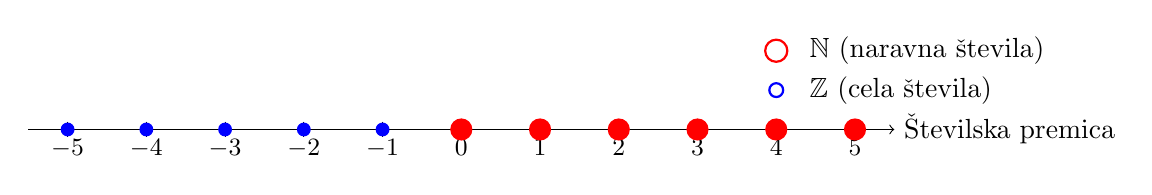
\begin{tikzpicture}[scale=1]
  \draw[->] (-5.5,0) -- (5.5,0) node[right] {Številska premica};
 
  \foreach \x in {-5,...,5} {
    \draw (\x,0.1) -- (\x,-0.1);
    \node[below] at (\x,0) {\small $\x$};
  }
  
  \foreach \x in {-5,...,5} {
    \fill[blue] (\x,0) circle (2.5pt);
  }
  
  \foreach \x in {0,...,5} {
    \fill[red] (\x,0) circle (4pt);
  }
  
  \draw[red, thick] (4,1) circle (4pt);
  \node[right] at (4.3,1) {$\mathbb{N}$ (naravna števila)};
  
  \draw[blue, thick] (4,0.5) circle (2.5pt);
  \node[right] at (4.3,0.5) {$\mathbb{Z}$ (cela števila)};
\end{tikzpicture}
}
\end{tabularx}


\begin{tabularx}{\textwidth}{X r}
\vprasanje{Naštejte računske operacije v množici $\mathbb{N}$}{1 točka}
\odgovor{%
V množici $\mathbb{N}$ je definirano \textbf{seštevanje, množenje, in potenciranje}. Odštevanje in deljenje nista vedno možna znotraj $\mathbb{N}$, saj rezultat ni vedno naravno število.
}
\end{tabularx}

\razmak{1em}

\begin{tabularx}{\textwidth}{X r}
\vprasanje{Definirajte odštevanje v množici $\mathbb{Z}$.}{1 točka}
\odgovor{%
V množici $\mathbb{Z}$ je odštevanje vedno možno, saj za vsako celo število $a$ in $b$ ($a, b \in \mathbb{Z}$) obstaja tudi njuna razlika $a - b$ v $\mathbb{Z}$. Rezultat odštevanja je lahko pozitiven, negativen ali enak $0$.
}
\end{tabularx}



\begin{tabularx}{\textwidth}{X r}
\vprasanje{Napišite vseh pet osnovnih računskih zakonov o seštevanju in množenju v množicah $\mathbb{N}$ in $\mathbb{Z}$}{3 točke}
\odgovor{%
Osnovni računski zakoni:
\begin{enumerate}
  \item \textbf{Komutativnost:} $a + b = b + a$, \quad $a \cdot b = b \cdot a$
  \item \textbf{Asociativnost:} $(a + b) + c = a + (b + c)$, \quad $(a \cdot b) \cdot c = a \cdot (b \cdot c)$
  \item \textbf{Distributivnost:} $a \cdot (b + c) = a \cdot b + a \cdot c$
  \item \textbf{Seštevanje z 0:} $a + 0 = a$
  \item \textbf{Množenje z 1:} $a \cdot 1 = a$
\end{enumerate}
}
\end{tabularx}

\razmak{0.5em}


% ******** 6. Liha in soda števila ********
\crta

\naslov{Liha in soda števila}

\begin{tabularx}{\textwidth}{X r}
\vprasanje{Definirajte soda in liha števila.}{2 točki}
\odgovor{%
\begin{itemize}

	\item \textbf{Soda števila} so cela števila, pri katerih je ostanek pri deljenju z $2$ enak $0$. Zapišemo jih kot $n = 2k$, kjer je $k \in \mathbb{Z}$.
	\item \textbf{Liha števila} so cela števila, pri katerih je ostanek pri deljenju z $2$ enak $1$. Zapišemo jih kot $n = 2k + 1$, kjer je $k \in \mathbb{Z}$.
	
\end{itemize}
}
\end{tabularx}

\begin{tabularx}{\textwidth}{X r}
\vprasanje{Pokažite, da je vsota dveh lihih števil sodo število.}{2 točki}
\odgovor{%
Naj bosta $a = 2k + 1$ in $b = 2m + 1$ dve lihi števili, kjer sta $k, m \in \mathbb{Z}$.

Potem je njuna vsota:
\[
a + b = (2k + 1) + (2m + 1) = 2k + 2m + 2 = 2(k + m + 1)
\]

Ker je rezultat deljiv z $2$, je vsota lihih števil sodo število.
}

\razmak{1em}

\end{tabularx}

\begin{tabularx}{\textwidth}{X r}
\vprasanje{Pokažite, da je kvadrat lihega števila liho število.}{2 točki}
\odgovor{%
Naj bo $a = 2k + 1$ liho število, kjer je $k \in \mathbb{Z}$.

Potem je kvadrat:
\[
a^2 = (2k + 1)^2 = 4k^2 + 4k + 1 = 2(2k^2 + 2k) + 1
\]

Ker je rezultat oblike $2n + 1$, je kvadrat lihega števila spet liho število.
}
\end{tabularx}
\razmak{0.5em}


% ******** 7. Praštevila ********
\crta

\naslov{Praštevila}

\begin{tabularx}{\textwidth}{X r}
\vprasanje{Definirajte praštevila in sestavljena števila. Zapišite množico vseh praštevil, ki so manjša od 20.}{2 točki}
\odgovor{%
\begin{itemize}
	\item \textbf{Praštevila} so naravna števila, večja od $1$, ki imajo točno dva delitelja: $1$ in samih sebe.

	\item \textbf{Sestavljena števila} so naravna števila, večja od $1$, ki imajo več kot dva delitelja (poleg $1$ in sebe še kakšnega drugega).

	\item Praštevila manjša od $20$ so:
$$\{2, 3, 5, 7, 11, 13, 17, 19\}$$
\end{itemize}
}
\end{tabularx}

\begin{tabularx}{\textwidth}{X r}
\vprasanje{Kaj je razcep naravnega števila na prafaktorje? Ali je razcep na prafaktorje enoličen? Koliko je praštevil?}{3 točke}
\odgovor{%
\begin{itemize}
	\item Razcep naravnega števila na prafaktorje pomeni, da število zapišemo kot produkt praštevil. Primer: $60 = 2 \cdot 2 \cdot 3 \cdot 5 = 2^2 \cdot 3 \cdot 5$

	\item Po osnovnem izreku aritmetike je razcep vsakega naravnega števila na prafaktorje \textbf{enoličen}, razen vrstnega reda faktorjev.

	\item Praštevil je \textbf{neskončno mnogo} (Evklidov izrek).
\end{itemize}
}
\end{tabularx}

\begin{tabularx}{\textwidth}{X r}
\vprasanje{Opišite enega izmed postopkov za preverjanje, ali je dano število praštevilo.}{1 točka}
\odgovor{%

Eden izmed postopkov je naslednji:
	\begin{itemize}
		\item Če želimo preveriti, ali je naravno število $n$ praštevilo, delimo $n$ z vsemi praštevili manjšimi ali enakimi $\sqrt{n}$. Če nobeno izmed njih ne deli števila $n$, potem je število $n$ praštevilo.
		\item \textbf{Primer}: Število $29$. ${\sqrt{29} \approx 5}$. $29$ ni deljivo z $2$, $3$ ali $5$, kar pomeni, da je praštevilo.
	\end{itemize}
}
\end{tabularx}

\razmak{0.5em}


% ******** 8. Deljivost ********
\crta

\naslov{Deljivost}

\begin{tabularx}{\textwidth}{X r}
\vprasanje{Kdaj je naravno število a večkratnik naravnega števila $b$?}{1 točka}
\odgovor{%
Naravno število $a$ je večkratnik naravnega števila $b$, če obstaja naravno število $k$, tako da velja:
$$a = k \cdot b$$
V tem primeru rečemo, da je $a$ deljivo z $b$.
}
\end{tabularx}

\razmak{1em}

\begin{tabularx}{\textwidth}{X r}
\vprasanje{Definirajte relacijo deljivosti v množici $\mathrm{N}$.}{1 točka}
\odgovor{%

Relacija deljivosti v množici $\mathrm{N}$ je definirana naslednje:
\begin{itemize}
	\item Za števili $a, b \in \mathrm{N}$ rečemo, da $a$ deli $b$ (zapišemo kot $a \mid b$), če obstaja $k \in \mathrm{N}$, tako da je $b = a \cdot k$. Gre za binarno relacijo na množici naravnih števil, ki je refleksivna, antisimetrična in tranzitivna.
\end{itemize}
}
\end{tabularx}

\begin{tabularx}{\textwidth}{X r}
\vprasanje{Opišite tri lastnosti relacije deljivosti}{3 točke}
\odgovor{%
Relacija deljivosti v $\mathrm{N}$ ima naslednje lastnosti:
\begin{itemize}
  \item \textbf{Refleksivnost:} Za vsako $a \in \mathrm{N}$ velja $a \mid a$.
  \item \textbf{Tranzitivnost:} Če $a \mid b$ in $b \mid c$, potem velja tudi $a \mid c$.
  \item \textbf{Antisimetričnost:} Če $a \mid b$ in $b \mid a$, potem velja $a = b$.
\end{itemize}
}
\end{tabularx}

\begin{tabularx}{\textwidth}{X r}
\vprasanje{Zapišite tri naravna števila $a, b$ in $c$, večja od 10 , da bo veljalo: $a$ deli $b$ in $b$ ne deli $c$.}{1 točka}
\odgovor{%
Primer:
$$a = 12,\quad b = 36,\quad c = 50$$

Tukaj velja: $12 \mid 36$ (ker $36 = 12 \cdot 3$), vendar $36 \nmid 50$ (ker $50 : 36$ ni celo število).
}
\end{tabularx}

\razmak{0.5em}


% ******** 9. Večkratniki in deljitelji ********
\crta

\naslov{Večkratniki in deljitelji}

\begin{tabularx}{\textwidth}{X r}
\vprasanje{Definirajte največji skupni delitelji dveh naravnih števil. Razložite metodo za izračun največjega skupnega delitelja dveh naravnih števil. Kdaj sta si dve naravni števili tuji?}{3 točke}
\odgovor{%
\begin{itemize}
	\item \textbf{Največji skupni delitelj} dveh naravnih števil $a$ in $b$ je največje naravno število, ki deli oba: $d = \max\{k \in \mathbb{N} \mid k \mid a \text{ in } k \mid b\}$.

	\item \textbf{Metoda za izračun:} Evklidov algoritem
	\begin{enumerate}
  		\item Če $a > b$, izračunaj $a \bmod b$ (ostanek pri deljenju).
  		\item Zamenjaj $a$ z $b$, $b$ z ostankom.
  		\item Ponavljaj, dokler ostanek ni $0$.
  		\item Zadnji ostanek v Evklidovem algoritmu je največji skupni delitelj ($r \neq 0$).
	\end{enumerate}

	\item \textbf{Tuji števili} sta $a$ in $b$, če je njun največji skupni delitelj enak $1$.
\end{itemize}
}
\end{tabularx}

\begin{tabularx}{\textwidth}{X r}
\vprasanje{Definirajte najmanjši skupni večkratnik dveh naravnih števil. Razložite metodo za izračun najmanjšega skupnega večkratnika dveh naravnih števil.}{2 točki}
\odgovor{%
\begin{itemize}
	\item \textbf{Najmanjši skupni večkratnik} dveh naravnih števil $a$ in $b$ je najmanjše naravno število, ki je deljivo z obema.

	\item \textbf{Formula za izračun} (NSD $=$ največji skupni deljitelj, NSV $=$ najmanjši skupni večkratnik):
	\[
	\mathrm{NSV}(a, b) = \frac{a \cdot b}{\mathrm{NSD}(a, b)}, \quad \mathrm{NSD(a,b)} \neq 0
	\]

	\item Najprej poiščemo največji skupni deljitelj, nato uporabimo zgornjo formulo za izračun najmanjši skupni večkratnik.
\end{itemize}
}
\end{tabularx}

\begin{tabularx}{\textwidth}{X r}
\vprasanje{Izberite različni naravni števili med 20 in 50 . Določite njun največji skupni delitelj in najmanjši skupni večkratnik.}{1 točka}
\odgovor{%
Naj bo $a = 36$ in $b = 48$.

\begin{itemize}
  \item $\mathrm{NSD}(36, 48) = 12$
  \item $\mathrm{NSV}(36, 48) = \dfrac{36 \cdot 48}{12} = 144$
\end{itemize}
}
\end{tabularx}

\razmak{0.5em}


% ******** 10. Deljenje naravnih števil ********
\crta

\naslov{Deljenje naravnih števil}

\begin{tabularx}{\textwidth}{X r}
\vprasanje{Povejte osnovni izrek o deljenju naravnih števil.}{2 točki}
\odgovor{%
Za poljubni naravni števili $a$ in $b$, kjer $b \ne 0$, obstajata natanko določeni naravni števili $q$ (količnik) in $r$ (ostanek), tako da velja:

\[
a = b \cdot q + r,\quad \text{kjer } 0 \le r < b
\]

To je osnovni izrek o deljenju naravnih števil.
}
\end{tabularx}

\razmak{1em}

\begin{tabularx}{\textwidth}{X r}
\vprasanje{Izberite naravno število med 5 in 10 ter naštejte elemente množice vseh ostankov pri deljenju z izbranim naravnim številom.}{2 točki}
\odgovor{%
Izberimo število $k = 7$. Množica vseh možnih ostankov pri deljenju z $7$ je:
\[
\{0, 1, 2, 3, 4, 5, 6\}
\]

Gre za vsa števila $r$, ki ustrezajo pogoju $0 \le r < 7$.
}
\end{tabularx}

\razmak{1em}

\begin{tabularx}{\textwidth}{X r}
\vprasanje{Naj bo $k$ naravno število. Opišite množico vseh ostankov pri deljenju z naravnim številom $k$.}{2 točki}
\odgovor{%
Za poljubno naravno število $k$ je množica vseh možnih ostankov pri deljenju z $k$:

\[
\{0, 1, 2, \dots, k - 1\}
\]

Gre za vsa števila $r$, ki izpolnjujejo pogoj $0 \le r < k$ v osnovnem izreku o deljenju.
}
\end{tabularx}

\razmak{1em}


% ******** 11. Kriterij deljivosti ********
\crta

\naslov{Kriterij deljivosti}

\begin{tabularx}{\textwidth}{X r}
\vprasanje{Za vsako izmed števil 2, 4 in 8 navedite kriterij deljivosti s tem številom.}{3 točke}
\odgovor{%
\begin{itemize}
  \item \textbf{Deljivost z 2:} Število je deljivo z $2$, če se konča na sodo števko (0, 2, 4, 6, 8).
  \item \textbf{Deljivost s 4:} Število je deljivo s $4$, če sta zadnji dve števki deljivi s $4$.
  \item \textbf{Deljivost z 8:} Število je deljivo z $8$, če so zadnje tri števke deljive z $8$.
\end{itemize}
}
\end{tabularx}

\begin{tabularx}{\textwidth}{X r}
\vprasanje{Navedite kriterij deljivosti s številom 3.}{1 točka}
\odgovor{%
\begin{itemize}
	\item Število je deljivo s $3$, če je vsota vseh njegovih števk deljiva s $3$.
\end{itemize}
}
\end{tabularx}

\begin{tabularx}{\textwidth}{X r}
\vprasanje{Navedite kriterij deljivosti s številom 6.}{1 točka}
\odgovor{%
\begin{itemize}
	\item Število je deljivo s $6$, če je hkrati deljivo z $2$ \textbf{in} z $3$.
\end{itemize}
\[
(2 \mid n \land 3 \mid n) \implies 6 \mid n
\]

}
\end{tabularx}

\begin{tabularx}{\textwidth}{X r}
\vprasanje{Poišcite primer štirimestnega naravnega števila, ki je deljivo s 6.}{1 točka}
\odgovor{%
\begin{itemize}
\item \textbf{$1236$}. Deljivo je z $2$, ker se konča na $6$, in z $3$, ker je vsota števk $1 + 2 + 3 + 6 = 12$, kar je deljivo s $3$.
\end{itemize}
}
\end{tabularx}

\razmak{0.5em}


% ******** 12. Ulomki in racionalna števila ********
\crta

\naslov{Ulomki in racionalna števila}

\begin{tabularx}{\textwidth}{X r}
\vprasanje{Kaj je ulomek? Kdaj dva ulomka predstavljata isto racionalno število?}{2 točki}
\odgovor{%
\begin{itemize}
\item \textbf{Ulomek} je zapis oblike $\dfrac{a}{b}$, kjer sta $a$ in $b$ celi števili, $b \ne 0$. Pomeni del celote ali razmerje med dvema številoma.

	\item Dva ulomka predstavljata isto racionalno število, če sta enaka po vrednosti. To velja, če je:
\[
\dfrac{a}{b} = \dfrac{c}{d} \iff a \cdot d = b \cdot c
\]
	To pomeni, da ju lahko zapišemo kot ekvivalentna ulomka (skrajšamo ali razširimo z istim številom).
\end{itemize}
}
\end{tabularx}

\begin{tabularx}{\textwidth}{X r}
\vprasanje{Pojasnite, kako ulomke seštevamo, odštevamo, množimo in delimo.}{4 točke}
\odgovor{%
\begin{itemize}
  \item \textbf{Seštevanje:} Ulomke pretvorimo na skupni imenovalec:
  \[
  \dfrac{a}{b} + \dfrac{c}{d} = \dfrac{a \cdot d + b \cdot c}{b \cdot d}
  \]
  \item \textbf{Odštevanje:} Podobno kot seštevanje, uporabimo skupni imenovalec:
  \[
  \dfrac{a}{b} - \dfrac{c}{d} = \dfrac{a \cdot d - b \cdot c}{b \cdot d}
  \]
  \item \textbf{Množenje:} Števec z števcem, imenovalec z imenovalcem:
  \[
  \dfrac{a}{b} \cdot \dfrac{c}{d} = \dfrac{a \cdot c}{b \cdot d}
  \]
  \item \textbf{Deljenje:} Prvi ulomek pomnožimo z obratom drugega:
  \[
  \dfrac{a}{b} \div \dfrac{c}{d} = \dfrac{a}{b} \cdot \dfrac{d}{c} = \dfrac{a \cdot d}{b \cdot c},\quad c \ne 0
  \]
\end{itemize}
}
\end{tabularx}

\razmak{0.5em}

% ******** 13. Ulomki in decimalni zapis ********
\crta

\naslov{Ulomki in decimalni zapis}

\begin{tabularx}{\textwidth}{X r}
\vprasanje{Kako iz decimalnega zapisa števila prepoznamo, da lahko to število zapišemo z ulomkom? Kako poljubnemu ulomku priredimo njegov decimalni zapis?}{2 točki}
\odgovor{%
\begin{itemize}
	\item Decimalno število lahko zapišemo z ulomkom, če je:
	\begin{itemize}
  		\item končno decimalno število (npr. $0{,}25$), ali
  		\item periodično decimalno število (npr. $0{,}333\ldots$).
	\end{itemize}
	\item Vsako končno ali periodično decimalno število je \textbf{racionalno} in ga lahko zapišemo z ulomkom. Poljubnemu ulomku $\dfrac{a}{b}$ priredimo decimalni zapis tako, da izvedemo običajno deljenje števca z imenovalcem, oziroma $a$ z $b$.
\end{itemize}
}
\end{tabularx}

\begin{tabularx}{\textwidth}{X r}
\vprasanje{Kateri ulomki imajo končen decimalni zapis? Povejte primer ulomka, ki nima končnega decimalnega zapisa.}{2 točki}
\odgovor{%

Ulomek $\frac{a}{b}$ ima končen decimalni zapis, če imenovalec $b$ (v skrajšani obliki) vsebuje le praštevili $2$ in/ali $5$ kot prafaktorja.
\begin{itemize}
	\item Primer končnega decimalnega zapisa: $\dfrac{3}{8} = 0{,}375$
	\item Primer ulomka brez končnega decimalnega zapisa: $\dfrac{1}{3} = 0{,}\overline{3}$
\end{itemize}
}
\end{tabularx}

\begin{tabularx}{\textwidth}{X r}
\vprasanje{Povejte primer periodičnega decimalnega števila (z dolžino periode vsaj dva) in ga zapišite kot ulomek.}{2 točki}
\odgovor{%

Primer periodičnega decimalnega števila. Naj bo $a = 0{,}\overline{142857}$ (dolžina periode je $6$)

Zapis kot ulomek:
\[
a = \dfrac{1}{7}
\]
}
\end{tabularx}

\razmak{0.5em}

% ******** 14. Realna števila ********
\crta

\naslov{Realna števila}

\begin{tabularx}{\textwidth}{X r}
\vprasanje{Kdaj je realno število racionalno in kdaj iracionalno? Kako se razlikujeta njuna decimalna zapisa?}{2 točki}
\odgovor{%
\begin{itemize}
	\item \textbf{Racionalno število} je realno število, ki ga lahko zapišemo kot ulomek $\dfrac{a}{b}$, kjer sta $a \in \mathbb{Z}$ in $b \in \mathbb{N}$, $b \ne 0$.

	\item \textbf{Iracionalno število} je realno število, ki ga \textbf{ni možno} zapisati kot ulomek dveh celih števil.

	\item Razlika v decimalnem zapisu:
	\begin{itemize}
  		\item Racionalna števila imajo končen ali periodičen decimalni zapis.
  		\item Iracionalna števila imajo neskončen, neperiodičen decimalni zapis.
	\end{itemize}
\end{itemize}
}
\end{tabularx}

\begin{tabularx}{\textwidth}{X r}
\vprasanje{Povejte primer racionalnega števila in dva primera iracionalnih števil.}{2 točki}
\odgovor{%

\textbf{Primer racionalnega števila:} $\dfrac{5}{8} = 0{,}625$

\textbf{Primera iracionalnih števil:}
\[
e \approx 2{,}71828\ldots,\quad \pi \approx 3{,}14159\ldots
\]

Oba imata neskončen, neponavljajoč decimalni zapis.
}
\end{tabularx}

\razmak{1em}

\begin{tabularx}{\textwidth}{X r}
\vprasanje{Opišite konstrukcijo točke na številski premici, ki predstavlja vrednost ulomka $\frac{m}{n}, m<n$, kjer sta $m$ in $n$ naravni števili in je $n>2$.}{2 točki}
\odgovor{%
Postopek konstrukcije ulomka $\dfrac{m}{n}$ na številski premici:
\begin{enumerate}
  \item Na premici označimo točki $0$ in $1$ (enoto).
  \item Interval med $0$ in $1$ razdelimo na $n$ enakih delov.
  \item Od začetka (točke $0$) označimo $m$-ti del.
\end{enumerate}
Tako dobljena točka na premici predstavlja ulomek $\dfrac{m}{n}$.
}
\end{tabularx}

\razmak{0.5em}


% ******** 15. Absolutna vrednost ********
\crta

\naslov{Absolutna vrednost}

\begin{tabularx}{\textwidth}{X r}
\vprasanje{Definirajte absolutno vrednost realnega števila in pojasnite njen geometrijski pomen.}{2 točki}
\odgovor{%
\begin{itemize}
	\item \textbf{Absolutna vrednost} realnega števila $x$ je:
\[
|x| =
\begin{cases}
x, & \text{če } x \geq 0 \\
-x, & \text{če } x < 0
\end{cases}
\]
	
	\item \textbf{Geometrijski pomen:} Absolutna vrednost števila $x$ je njegova razdalja od točke $0$ na številski premici.
\end{itemize}
}

\end{tabularx}

\razmak{1em}

\begin{tabularx}{\textwidth}{X r}
\vprasanje{Naj bosta $a$ in $b$ realni števili. Kaj predstavlja število $|b-a|$ ?}{1 točka}
\odgovor{%
\begin{itemize}
	\item Število $|b - a|$ predstavlja razdaljo med točkama $a$ in $b$ na številski premici, ne glede na vrstni red.
\end{itemize}
}
\end{tabularx}

\begin{tabularx}{\textwidth}{X r}
\vprasanje{Na številski premici pojasnite rešitev enačbe $|x|=a$, kjer je $a$ pozitivno realno število. Odgovor ponazorite s primerom.}{1 točka}
\odgovor{%

\begin{itemize}
	\item Enačba $|x| = a$ ima dve rešitvi:
	\[
	x = a \quad \text{ali} \quad x = -a
	\]

To pomeni, da je $x$ oddaljen od $0$ za $a$ enot.

	\item \textbf{Primer:} $|x| = 3$ ima rešitvi $x = 3$ in $x = -3$.
\end{itemize}
}
\end{tabularx}

\begin{tabularx}{\textwidth}{X r}
\vprasanje{Naj bosta $a$ in $b$ realni števili. Primerjajte izraza $|a|+|b|$ ter $|a+b|$. Odgovor ponazorite s primeri.}{2 točki}
\odgovor{%

Vedno velja:
\[
|a + b| \le |a| + |b|
\]
To je trikotniška neenakost. Dolžina ene stranice $|a+b|$ bo vedno manjša oziroma enaka vsoti dolžin ostalih dveh stranic $|a| + |b|$.
\razmak{0.5em}

\textbf{Primer 1 (enakost):} $a = 2$, $b = 3$:
\[
|a + b| = |5| = 5,\quad |a| + |b| = 2 + 3 = 5
\]

\textbf{Primer 2 (stroga neenakost):} $a = 4$, $b = -6$:
\[
|a + b| = |-2| = 2,\quad |a| + |b| = 4 + 6 = 10
\]
}
\end{tabularx}

\razmak{0.5em}


% ******** 16. Kompleksna števila ********
\crta

\naslov{Kompleksna števila}

\begin{tabularx}{\textwidth}{X r}
\vprasanje{Definirajte množico kompleksnih števil. Kako grafično upodobimo (predstavimo) kompleksna števila?}{2 točki}
\odgovor{%
\begin{itemize}
	\item \textbf{Množica kompleksnih števil} $\mathbb{C}$ je množica vseh števil oblike:
	\[
	z = a + bi,\quad \text{kjer sta } a, b \in \mathbb{R} \text{ in } i^2 = -1
	\]

	Število $a$ imenujemo realni del ($\operatorname{Re}(z)$), $b$ pa imaginarni del ($\operatorname{Im}(z)$).

\razmak{1em}

	\item \textbf{Grafična predstavitev:} Kompleksna števila predstavimo v \textbf{kompleksni ravnini}, kjer:
	\begin{itemize}
  		\item $x$-os predstavlja realni del,
  		\item $y$-os predstavlja imaginarni del.
	\end{itemize}
	Tako število $z = a + bi$ upodobimo kot točko s koordinatama $(a, b)$.
\end{itemize}
}
\end{tabularx}

\begin{tabularx}{\textwidth}{X r}
\vprasanje{Definirajte operacijo seštevanja v množici C. Opišite geometrijski pomen seštevanja kompleksnih števil.}{2 točki}
\odgovor{%
\begin{itemize}
	\item \textbf{Seštevanje kompleksnih števil:}

	Naj bo \( z_1 = a + bi \), \( z_2 = c + di \), in \( z_3 = z_1 + z_2 \), kjer \( z_1, z_2, z_3 \in \mathbb{C} \). Potem je
	\[
	z_3 = z_1 + z_2 = (a + c) + (b + d)i
	\]

	\item \textbf{Geometrijski pomen:} Seštevanje števil v kompleksni ravnini je vektorsko seštevanje. Če števili predstavimo kot vektorja iz izhodišča $(0,0)$, je njuna vsota glavna diagonalnega dobljenega paralelograma.
\end{itemize}
}
\end{tabularx}

\begin{tabularx}{\textwidth}{X r}
\vprasanje{V kompleksni ravnini predstavite podmnožici kompleksnih števil $A=\{z \in \mathbb{C} ; \operatorname{Im}(z)=2\}$ in $B=\{z \in \mathbb{C} ; \operatorname{Im}(z)=\operatorname{Re}(z)\}$.}{2 točki}
\odgovor{%
\begin{itemize}
	\item \textbf{Podmnožica $A$:} Vsa kompleksna števila z imaginarnim delom $2$. V kompleksni ravnini je to \textbf{vodoravna premica} pri $y = 2$.
	\item \textbf{Podmnožica $B$:} Vsa kompleksna števila, kjer sta imaginarni in realni del enaka ($\operatorname{Im}(z) = \operatorname{Re}(z)$). To je \textbf{premica skozi izhodišče} z enačbo $y = x$ (diagonala).
\end{itemize}
Obe podmnožici sta neskončni množici točk v kompleksni ravnini.

\medskip
\centering
\begin{tikzpicture}[scale=1]

  \draw[->] (-4,0) -- (4,0) node[right] {Re};
  \draw[->] (0,-1) -- (0,5) node[above] {Im};

  \foreach \x in {-3,-2,-1,1,2,3} {
    \draw (\x,0.1) -- (\x,-0.1) node[below] {\small $\x$};
  }
  \foreach \y in {1,2,3,4} {
    \draw (0.1,\y) -- (-0.1,\y) node[left] {\small $\y$};
  }

  \draw[red, thick] (-4,2) -- (4,2);
  \node[red, above right] at (3,2) {$A: \operatorname{Im}(z)=2$};

  \draw[blue, thick] (-3,-3) -- (4,4);
  \node[blue, above left] at (3,3) {$B: \operatorname{Im}(z)=\operatorname{Re}(z)$};

  \filldraw (0,0) circle (2pt) node[below left] {$0$};
\end{tikzpicture}
}
\end{tabularx}


\razmak{0.5em}


% ******** 17. Množenje kompleksnih števil ********
\crta

\naslov{Množenje kompleksnih števil}

\begin{tabularx}{\textwidth}{X r}
\vprasanje{Definirajte operacijo množenja v množici C. Zapišite primer.}{2 točki}
\odgovor{%
\begin{itemize}
	\item \textbf{Množenje kompleksnih števil:}

	Naj bo \( z_1 = a + bi \), \( z_2 = c + di \), in \( z_3 = z_1 \cdot z_2 \), kjer \( z_1, z_2, z_3 \in \mathbb{C} \). Potem je
	\[
	z_3 = z_1 \cdot z_2 = (a + bi)(c + di) = (ac - bd) + (ad + bc)i
	\]
	
	\item \textbf{Primer:}
	\[
	(2 + 3i)(1 + 4i) = 2 \cdot 1 + 2 \cdot 4i + 3i \cdot 1 + 3i \cdot 4i = 2 + 8i + 3i + 12i^2 = 2 + 11i - 12 = -10 + 11i
	\]
	
\end{itemize}
}
\end{tabularx}

\begin{tabularx}{\textwidth}{X r}
\vprasanje{Opišite geometrijski pomen množenja kompleksnega števila s številom -1 in geometrijski pomen množenja kompleksnega števila s pozitivnim realnim številom.}{2 točki}
\odgovor{%
\begin{itemize}
  \item \textbf{Množenje s $-1$} pomeni \textbf{zrcaljenje čez izhodišče} v kompleksni ravnini (obrat za $180^\circ$).
  \item \textbf{Množenje s pozitivnim realnim številom} pomeni \textbf{razteg ali stisk} v smeri od izhodišča. Vektor ostane v isti smeri, spremeni se le njegova dolžina.
\end{itemize}
}
\end{tabularx}

\begin{tabularx}{\textwidth}{X r}
\vprasanje{Naj bo $n$ naravno število. Izračunajte $i^*$, kjer je $n$ letošnja letnica.}{1 točka}
\odgovor{%
\begin{itemize}
	\item Naj bo $n$ enako letošnji letnici, potem je $n = 2025$.

	Ker potence imaginarne enote $i$ sledijo ciklu dolžine $4$:
	\[
	i^1 = i,\quad i^2 = -1,\quad i^3 = -i,\quad i^4 = 1,\quad \text{in nato se cikel ponavlja}
	\]

	Izračunamo ostanek:
	\[
	2025 \bmod 4 = 1 \Rightarrow i^{2025} = i^1 = i
	\]
\end{itemize}
}
\end{tabularx}

\begin{tabularx}{\textwidth}{X r}
\vprasanje{Izberite kompleksno število $z=a+b i$, kjer sta $a$ in $b$ od nič različni realni števili, in izračunajte $z^2$.}{1 točka}
\odgovor{%

Izberemo $z = 3 + 2i$.

Izračunamo:
\[
z^2 = (3 + 2i)^2 = 9 + 12i + 4i^2 = 9 + 12i - 4 = 5 + 12i
\]
}
\end{tabularx}

\razmak{0.5em}


% ******** 18. Absolutna vrednost kompleksnega števila ********
\crta

\naslov{Absolutna vrednost kompleksnega števila}

\begin{tabularx}{\textwidth}{X r}
\vprasanje{Definirajte absolutno vrednost kompleksnega števila. Na primeru pokažite izračun absolutne vrednosti kompleksnega števila.}{2 točki}
\odgovor{%
\begin{itemize}
	\item \textbf{Absolutna vrednost} kompleksnega števila $z = a + bi$ je definirana kot:
	\[
	|z| = \sqrt{a^2 + b^2}
	\]

	\item \textbf{Primer:} Naj bo $z = 3 - 4i$. Potem je:
	\[
	|z| = \sqrt{3^2 + (-4)^2} = \sqrt{9 + 16} = \sqrt{25} = 5
	\]
To je enako dolžini od izhodišča $(0,0)$ v kompleksni ravnini.
\end{itemize}
}
\end{tabularx}

\razmak{1em}

\begin{tabularx}{\textwidth}{X r}
\vprasanje{Na primeru izbranega kompleksnega števila $z=a+b i$, kjer je $a \neq 0$ in $b \neq 0$, pokažite, da je $|2 z|=|2|z$.}{2 točki}
\odgovor{%
\begin{itemize}
	\item Naj bo $z = 1 + 2i$. Potem je $2z = 2(1 + 2i) = 2 + 4i$.

Izračunajmo:
\[
|2z| = |2 + 4i| = \sqrt{2^2 + 4^2} = \sqrt{4 + 16} = \sqrt{20}
\]

Po drugi strani:
\[
|2| \cdot |z| = 2 \cdot |1 + 2i| = 2 \cdot \sqrt{1^2 + 2^2} = 2 \cdot \sqrt{1 + 4} = 2 \cdot \sqrt{5}
\]

Ker $\sqrt{20} = 2\sqrt{5}$, sledi:
\[
|2z| = |2| \cdot |z|
\]
\end{itemize}
}
\end{tabularx}

\begin{tabularx}{\textwidth}{X r}
\vprasanje{V kompleksni ravnini predstavite množico točk $\{z \in \mathrm{C} ;|z| \leq 3\}$. Zapišite primer kompleksnega števila $z=a+b i$ iz te množice, kjer je $a$ pozitivno, $b$ pa negativno realno število.}{2 točki}
\odgovor{%

\begin{itemize}
	\item Množica $\{z \in \mathbb{C} \mid |z| \leq 3\}$ so vse točke v kompleksni ravnini z razdaljo največ $3$ od izhodišča. Geometrijsko je to \textbf{krog s središčem v izhodišču in polmerom $3$}, vključno z notranjostjo.

\item \textbf{Primer števila:} $z = 2 - i$

Izračun:
\[
|z| = \sqrt{2^2 + (-1)^2} = \sqrt{4 + 1} = \sqrt{5} \approx 2{,}24 < 3
\]

Torej $z = 2 - i$ pripada tej množici, $a > 0$, $b < 0$.
\end{itemize}
}
\end{tabularx}

\razmak{0.5em}


% ******** 19. Konjugirana vrednost kompleksnega števila ********
\crta

\naslov{Konjugirana vrednost kompleksnega števila}

\begin{tabularx}{\textwidth}{X r}
\vprasanje{Definirajte konjugirano vrednost kompleksnega števila in razložite njen geometrijski pomen.}{2 točki}
\odgovor{%

\begin{itemize}
	\item \textbf{Konjugirana vrednost} kompleksnega števila $z = a + bi$ (kjer sta $a, b \in \mathbb{R}$) je:
	\[
	\overline{z} = a - bi
	\]

	\item \textbf{Geometrijski pomen:} Konjugiranje kompleksnega števila je \textbf{zrcaljenje čez realno os} v kompleksni ravnini. To pomeni, da imata točki $z$ in $\overline{z}$ enak realni del, ampak nasprotna imaginarna dela.
\end{itemize}
}
\end{tabularx}

\begin{tabularx}{\textwidth}{X r}
\vprasanje{Dokažite, da je konjugirana vrednost vsote dveh kompleksnih števil enaka vsoti njunih konjugiranih vrednosti.}{2 točki}
\odgovor{%
\begin{itemize}
	\item Naj bo $z_1 = a + bi$, $z_2 = c + di$, kjer $z_1, z_2 \in \mathbb{C}$.

Potem je:
\[
z_1 + z_2 = (a + c) + (b + d)i
\]

Konjugirana vrednost:
\[
\overline{z_1 + z_2} = (a + c) - (b + d)i
\]

Po drugi strani:
\[
\overline{z_1} = a - bi,\quad \overline{z_2} = c - di,\quad \overline{z_1} + \overline{z_2} = (a + c) - (b + d)i
\]

Torej:
\[
\overline{z_1 + z_2} = \overline{z_1} + \overline{z_2}
\]
\end{itemize}
}
\end{tabularx}

\begin{tabularx}{\textwidth}{X r}
\vprasanje{Izberite kompleksno število $z=a+b i$, kjer sta $a$ in $b$ od nič različni realni števili, in izračunajte $z^{-1}$.}{2 točki}
\odgovor{%
\begin{itemize}
\item Izberimo $z = 1 + 2i$.

Obratno število izračunamo tako, da pomnožimo števec in imenovalec z njegovo konjugirano vrednostjo:
\[
z^{-1} = \frac{1}{z} = \frac{1}{1 + 2i} \cdot \frac{1 - 2i}{1 - 2i} = \frac{1 - 2i}{1^2 + 2^2} = \frac{1 - 2i}{5} = \frac{1}{5} - \frac{2}{5}i
\]
Torej:
\[
z^{-1} = \frac{1}{5} - \frac{2}{5}i
\]
\end{itemize}
}
\end{tabularx}

\razmak{0.5em}


% ******** 20. Enačbe ********
\crta

\naslov{Enačbe}

\begin{tabularx}{\textwidth}{X r}
\vprasanje{Kaj je enačba in kaj je rešitev enačbe? Kdaj sta dve enačbi ekvivalentni (enakovredni)?}{2 točki}
\odgovor{%
\begin{itemize}
	\item \textbf{Enačba} je matematična izjava, v kateri sta dve izraza povezana z enačajem ($=$) in vsaj en izraz vsebuje neznanko.

	\item \textbf{Rešitev enačbe} je vrednost spremenljivke, ki enačbo spremeni v pravilno trditev (resnično izjavo).

	\item \textbf{Ekvivalentni enačbi} imata enako množico rešitev. To pomeni, da vsaka rešitev ene enačbe zadošča kot rešitev druge enačbe.
\end{itemize}
}
\end{tabularx}

\begin{tabularx}{\textwidth}{X r}
\vprasanje{Opišite postopke, ki dano enačbo prevedejo v ekvivalentno enačbo.}{2 točki}
\odgovor{%
\begin{itemize}
	\item Enačbo lahko preoblikujemo v ekvivalentno enačbo z naslednjimi postopki:
	\begin{itemize}
	  \item Seštevanje ali odštevanje istega števila na obeh straneh.
	  \item Množenje ali deljenje obeh strani z istim številom $a$, kjer $a \neq 0$. 
	  \item Uporaba osnovnih računskih zakonov (distributivnost, komutativnost,...).
	  \item Poenostavljanje izrazov (odpravljanje oklepajev, krajšanje,...).
	\end{itemize}
\textbf{Ti postopki ne spremenijo množice rešitev.}
\end{itemize}
}
\end{tabularx}

\begin{tabularx}{\textwidth}{X r}
\vprasanje{Kako rešimo sistem dveh linearnih enačb z dvema neznankama? Zapišite primer takega sistema in ga rešite.}{2 točki}
\odgovor{%
\begin{itemize}
\item	Sistem rešujemo z:
\begin{itemize}
  \item metodo \textbf{substitucije} (enačimo, nadomestimo),
  \item metodo \textbf{odštevanja ali seštevanja} (eliminiramo spremenljivko),
\end{itemize}

\textbf{Primer:}
\[
\begin{cases}
x + y = 5 \\
2x - y = 4
\end{cases}
\]

\textbf{Rešitev:} Seštejemo enačbi:
\[
(x + y) + (2x - y) = 5 + 4 \Rightarrow 3x = 9 \Rightarrow x = 3
\]

Vstavimo v prvo enačbo: $3 + y = 5 \Rightarrow y = 2$

\textbf{Rešitev sistema:} $x = 3$, $y = 2$
\end{itemize}
}
\end{tabularx}

\razmak{0.5em}


% ******** 21. Potence z celimi eksponenti ********
\crta

\naslov{Potence z celimi eksponenti}

\begin{tabularx}{\textwidth}{X r}
\vprasanje{Definirajte potenco $z$ naravnim in potenco $s$ celim eksponentom.}{1 točka}
\odgovor{%
\begin{itemize}
	\item \textbf{Potenca z naravnim eksponentom:} Za $a \in \mathbb{R}$ in $n \in \mathbb{N}$ definiramo:
	\[
	a^n = a \cdot a \cdot \dots \cdot a \quad (n\text{-krat})
	\]

	\item \textbf{Potenca s celim eksponentom:} Če je $n \in \mathbb{Z}$, $a \ne 0$, potem velja:
	\[
	a^{-n} = \frac{1}{a^n}
	\]

Za $a^0$ (kjer $a \ne 0$) velja:
\[
a^0 = 1
\]
\end{itemize}
}
\end{tabularx}

\begin{tabularx}{\textwidth}{X r}
\vprasanje{Naštejte tri pravila za računanje s potencami s celimi eksponenti.}{3 točka}
\odgovor{%
\begin{enumerate}
  \item $a^m \cdot a^n = a^{m+n}$ \quad (množenje z enakimi osnovami)
  \item $\dfrac{a^m}{a^n} = a^{m-n}$ \quad (deljenje z enakimi osnovami, $a \ne 0$)
  \item $(a^m)^n = a^{m \cdot n}$ \quad (potenca potence)
\end{enumerate}
}
\end{tabularx}

\begin{tabularx}{\textwidth}{X r}
\vprasanje{Na primerih potenc s celimi eksponenti pokažite uporabo dveh izmed zgomjih pravil.}{2 točki}
\odgovor{%
\begin{itemize}
	\item \textbf{Primer 1 (množenje):}
	\[
	2^3 \cdot 2^4 = 2^{3+4} = 2^7 = 128
	\]

	\item \textbf{Primer 2 (deljenje):}
	\[
	5^6 \div 5^2 = 5^{6-2} = 5^4 = 625
	\]
\end{itemize}
}
\end{tabularx}
\razmak{0.5em}


% ******** 22. Koreni ********
\crta

\naslov{Koreni}

\begin{tabularx}{\textwidth}{X r}
\vprasanje{Definirajte $\sqrt[n]{x}$ za poljubno naravno število $n$. Zakaj je pomembno, ali je $n$ sodo ali liho število?}{2 točki}
\odgovor{%
\begin{itemize}
	\item Za poljubno naravno število $n$ in realno število $x$ definiramo:
\[
\sqrt[n]{x} = y \iff y^n = x
\]

	\begin{itemize}
		\item Če je $n$ \textbf{sodo}, potem $\sqrt[n]{x}$ obstaja le za $x \ge 0$ (rezultat je nenegativen).
		\item Če je $n$ \textbf{liho}, potem $\sqrt[n]{x}$ obstaja za vsako realno število $x$ (lahko tudi negativno), ker potenca lihe stopnje ohrani predznak. %%%% NI MI VSEC NI MI VSEC NI MI VSEC
	\end{itemize}
\end{itemize}
}
\end{tabularx}

\begin{tabularx}{\textwidth}{X r}
\vprasanje{Kako množimo korene z enakima in kako z različnima korenskima eksponentoma?}{1 točka}
\odgovor{%
\begin{itemize}
	\item \textbf{Enaka eksponenta:}
	\[
	\sqrt[n]{a} \cdot \sqrt[n]{b} = \sqrt[n]{a \cdot b}
	\]

	\item \textbf{Različna eksponenta:} Pretvorimo korene v potence:
	\[
	\sqrt[m]{a} \cdot \sqrt[n]{a} = a^{\frac{1}{m} + \frac{1}{n}}
	\]
	in nato izraz poenostavimo.
\end{itemize}
}
\end{tabularx}

\begin{tabularx}{\textwidth}{X r}
\vprasanje{Kako korenimo produkt? Kako korenimo korene?}{1 točka}
\odgovor{%
\begin{itemize}
	\item \textbf{Korenjenje produkta:}
	\[
	\sqrt[n]{a \cdot b} = \sqrt[n]{a} \cdot \sqrt[n]{b}
	\]

	\item \textbf{Korenjenje korena:}
	\[
	\sqrt[m]{\sqrt[n]{a}} = \sqrt[mn]{a}
	\]
\end{itemize}
}
\end{tabularx}

\begin{tabularx}{\textwidth}{X r}
\vprasanje{Racionalizirajte imenovalec ulomka $\frac{a}{a+\sqrt{b}}$.}{2 točka}
\odgovor{%
\begin{itemize}
	\item Imenovalec racionaliziramo tako, da ulomek pomnožimo z $(a - \sqrt{b}) / (a - \sqrt{b})$:

	\[
	\frac{a}{a + \sqrt{b}} \cdot \frac{a - \sqrt{b}}{a - \sqrt{b}} = \frac{a(a - \sqrt{b})}{a^2 - b}
	\]

	Tako dobimo:
	\[
	\frac{a(a - \sqrt{b})}{a^2 - b}
	\]

	Imenovalec je zdaj racionalno število.
\end{itemize}
}
\end{tabularx}

\razmak{0.5em}


% ******** 23. Potence z racionalnimi eksponenti ********
\crta

\naslov{Potence z racionalnimi eksponenti}

\begin{tabularx}{\textwidth}{X r}
\vprasanje{Definirajte potenco s pozitivno osnovo in racionalnim eksponentom.}{1 točka}
\odgovor{%
\begin{itemize}
	\item Za pozitivno realno število $a$ in racionalno število eksponent $r = \frac{m}{n}$ (kjer sta $m \in \mathbb{Z}$, $n \in \mathbb{N}$) definiramo:

\[
a^{\frac{m}{n}} = \sqrt[n]{a^m} = \left(\sqrt[n]{a}\right)^m
\]

Ta definicija omogoča razširitev pojma potence tudi na racionalne eksponente.
\end{itemize}
}
\end{tabularx}

\begin{tabularx}{\textwidth}{X r}
\vprasanje{Podajte primera dveh potenc z enakima osnovama in različnima pozitivnima racionalnima eksponentoma (ki nista celi števili) in izračunajte njun produkt. Izrazite ti dve potenci še kot korena in izračunajte njun produkt.}{3 točke}
\odgovor{%
\begin{itemize}
	\item Izberimo osnovo $a = 16$ in eksponenta $\frac{1}{2}$ ter $\frac{3}{4}$.

	\textbf{Potenčni zapis:}
	\[
	16^{\frac{1}{2}} \cdot 16^{\frac{3}{4}} = 16^{\frac{1}{2} + \frac{3}{4}} = 16^{\frac{5}{4}}
	\]

	\textbf{Zapis s koreni:}
	\[
	\sqrt{16} \cdot \sqrt[4]{16^3} = 4 \cdot \sqrt[4]{4096} = 4 \cdot 8 = 32
	\]

	Torej je produkt $32$.
\end{itemize}
}
\end{tabularx}

\razmak{0.5em}


% ******** 24. Premice ********
\crta

\naslov{Premice}

\begin{tabularx}{\textwidth}{X r}
\vprasanje{Definirajte vzporednost premic v ravnini.}{1 točka}
\odgovor{%
\begin{itemize}
	\item Dve premici v ravnini sta \textbf{vzporedni}, če ležita v isti ravnini in nimata nobene skupne točke (se ne sekata). Označimo: $p \parallel q$.
\end{itemize}
}
\end{tabularx}

\begin{tabularx}{\textwidth}{X r}
\vprasanje{Naštejte vse možne medsebojne lege dveh premic v ravnini.}{2 točki}
\odgovor{%
\begin{itemize}
	\item Dve premici v ravnini imata lahko naslednje medsebojne lege:
	\begin{itemize}
 		\item sekata se (imata eno skupno točko),
		\item sta vzporedni (nimata nobene skupne točke),
		\item sta identični (vse točke ene ležijo tudi na drugi).
	\end{itemize}
\end{itemize}
}
\end{tabularx}

\begin{tabularx}{\textwidth}{X r}
\vprasanje{Naštejte dve lastnosti relacije vzporednosti premic v ravnini.}{2 točki}
\odgovor{%
\begin{itemize}
	\item Relacija vzporednosti premic ima naslednji lastnosti:
	\begin{itemize}
	  \item \textbf{Refleksivnost:} Vsaka premica je vzporedna sama sebi ($p \parallel p$).
	  \item \textbf{Simetričnost:} Če je $p \parallel q$, potem je tudi $q \parallel p$.
	\end{itemize}
	(Opomba: relacija ni tranzitivna brez dodatnih geometrijskih pogojev.)
\end{itemize}
}
\end{tabularx}

\begin{tabularx}{\textwidth}{X r}
\vprasanje{Povejte aksiom o vzporednici.}{1 točka}
\odgovor{%
\begin{itemize}
	\item \textbf{Evklidov aksiom o vzporednici:}

Če je dana premica $p$, in točka $T$ izven te premice, potem skozi to točko poteka natanko ena premica, ki je vzporedna premici $p$.
\end{itemize}
}
\end{tabularx}

\razmak{0.5em}


% ******** 25. Koti ********
\crta

\naslov{Koti}

\begin{tabularx}{\textwidth}{X r}
\vprasanje{Pojasnite pojme ničelni, pravi, iztegnjeni in polni kot.}{2 točki}
\odgovor{%
\begin{itemize}
  \item \textbf{Ničelni kot:} kot z velikostjo $0^\circ$.
  \item \textbf{Pravi kot:} kot z velikostjo $90^\circ$.
  \item \textbf{Iztegnjeni kot:} kot z velikostjo $180^\circ$, njegova kraka ležita na isti premici.
  \item \textbf{Polni kot:} kot z velikostjo $360^\circ$.
\end{itemize}
}
\end{tabularx}

\begin{tabularx}{\textwidth}{X r}
\vprasanje{Pojasnite pojma sokota in sovršna kota.}{2 točki}
\odgovor{%
\begin{itemize}
	\item \textbf{Sokota} sta kota, ki imata skupni krak in skupaj tvorita kot $180^\circ$ (iztegnjeni kot).
	\item \textbf{Sovršna kota} sta kota, ki nastaneta pri sečišču dveh premic in imata skupni vrh ter nasprotna kraka. Sovršna kota sta vedno enaka.
\end{itemize}
}
\end{tabularx}

\begin{tabularx}{\textwidth}{X r}
\vprasanje{Kdaj je dani kot oster in kdaj top?}{1 točka}
\odgovor{%
\begin{itemize}
  \item \textbf{Oster kot:} kot, manjši od $90^\circ$.
  \item \textbf{Top kot:} kot, večji od $90^\circ$ in manjši od $180^\circ$.
\end{itemize}
}
\end{tabularx}

\begin{tabularx}{\textwidth}{X r}
\vprasanje{Kdaj sta kota komplementarna in kdaj suplementarna?}{1 točka}
\odgovor{%
\begin{itemize}
  \item \textbf{Komplementarna kota:} Kota $\alpha$ in $\beta$ z istim izhodiščem, njuna vsota je $90^\circ$.
  \item \textbf{Suplementarna kota:} Kota $\alpha$ in $\beta$ z istim izhodiščem, njuna vsota je $180^\circ$.
\end{itemize}
}
\end{tabularx}

\razmak{0.5em}


% ******** 26. Koti ********
\crta

\naslov{Koti}

\begin{tabularx}{\textwidth}{X r}
\vprasanje{Definirajte kotno stopinjo, kotno minuto in kotno sekundo.}{1 točka}
\odgovor{
\begin{itemize}
    \item Ena kotna stopinja ($1^\circ$) je $1/360$ polnega kroga oziroma obrata.
    \item Ena kotna minuta ($1'$) je $1/60$ kotne stopinje.
    \item Ena kotna sekunda ($1''$) je $1/60$ kotne minute.
\end{itemize}
}
\end{tabularx}

\begin{tabularx}{\textwidth}{X r}
\vprasanje{Definirajte radian.}{1 točka}
\odgovor{
\begin{itemize}
    \item En radian je velikost središčnega kota, ki na krožnici dolžine $r$ (polmer) odmeri lok dolžine $r$.
\end{itemize}
}
\end{tabularx}

\begin{tabularx}{\textwidth}{X r}
\vprasanje{Zapišite zvezo med stopinjami in radiani.}{1 točka}
\odgovor{
\begin{itemize}
    \item $\pi$ rad $= 180^\circ$, kjer je rad = radian.
    \item $1^\circ = \dfrac{\pi}{180}$ rad, kjer je rad = radian.
    \item $1$ rad $= \dfrac{180}{\pi}^\circ$, kjer je rad = radian.
\end{itemize}
}
\end{tabularx}

\begin{tabularx}{\textwidth}{X r}
\vprasanje{Koliko stopinj meri en radian?}{1 točka}
\odgovor{
\begin{itemize}
    \item En radian meri približno $57{,}296^\circ$, ker je $1$ rad $= \dfrac{180}{\pi}^\circ \approx 57,296^\circ$ 
\end{itemize}
}
\end{tabularx}

\begin{tabularx}{\textwidth}{X r}
\vprasanje{Koliko radianov merijo koti $30^{\circ}, 45^{\circ}, 60^{\circ}$ in $90^{\circ}$ ?}{1 točka}
\odgovor{
\begin{itemize}
    \item $30^\circ = \dfrac{\pi}{6}$ rad
    \item $45^\circ = \dfrac{\pi}{4}$ rad
    \item $60^\circ = \dfrac{\pi}{3}$ rad
    \item $90^\circ = \dfrac{\pi}{2}$ rad
\end{itemize}
}
\end{tabularx}

\begin{tabularx}{\textwidth}{X r}
\vprasanje{Kdaj sta kota skladna?}{1 točka}
\odgovor{
\begin{itemize}
    \item Kota sta skladna, če imata enako velikost oziroma enako merita v stopinjah ali radianih.
    \item V radianih: kota $\alpha$ in $\beta$ sta skladna $\iff \alpha \equiv \beta \pmod{2\pi}$
\end{itemize}
}
\end{tabularx}


\razmak{0.5em}

% ******** 27. Trikotnik ********
\crta

\naslov{Trikotnik}

\begin{tabularx}{\textwidth}{X r}
\vprasanje{Definirajte trikotnik.}{1 točka}
\odgovor{
\begin{itemize}
    \item Trikotnik je geometrijski lik, ki ga določajo tri točke, kjer vsaj en par ne leži na isti premici, ter daljice, ki te točke povezujejo. Je lik, ki zapre prostor in ima 3 kote, ki skupaj merijo $180^\circ$ (vsota notranjih kotov).
    \item Trikotnik ima tri stranice, tri oglišča in tri kote.
\end{itemize}
}
\end{tabularx}

\begin{tabularx}{\textwidth}{X r}
\vprasanje{Definirajte notranji in zunanji kot trikotnika.}{2 točki}
\odgovor{
\begin{itemize}
    \item Notranji kot trikotnika je kot, ki ga tvorita dve stranici trikotnika v istem oglišču.
    \item Zunanji kot trikotnika pri nekem oglišču je kot, ki ga tvorita stranica trikotnika in podaljšek sosednje stranice iz tega oglišča.
    \item Notranji in zunanji kot pri istem oglišču sta sosednja kota, ki skupaj tvorita iztegnjeni kot ($180^\circ$).
\end{itemize}
}
\end{tabularx}

\begin{tabularx}{\textwidth}{X r}
\vprasanje{Kolikšna je vsota notranjih kotov trikotnika? Trditev dokažite.}{2 točki}
\odgovor{
\begin{itemize}
    \item Vsota notranjih kotov trikotnika je $180^\circ$ oziroma $\pi$ radianov.
    \item \textbf{Dokaz:}
    \begin{itemize}
        \item Narišemo poljuben trikotnik in skozi eno oglišče (npr. $C$) potegnemo premico, ki je vzporedna nasprotni stranici $AB$.
        \item Zaradi izmeničnih kotov velja, da sta kota pri ogliščih $A$ in $B$ skladna z dvema kotoma ob tej vzporednici.
        \item Ker ti trije koti skupaj tvorijo iztegnjeni kot, je njihova vsota $180^\circ$.
    \end{itemize}
\end{itemize}
}
\end{tabularx}

\begin{tabularx}{\textwidth}{X r}
\vprasanje{Kolikšna je vsota zunanjih kotov trikotnika?}{1 točka}
\odgovor{
\begin{itemize}
    \item Vsota zunanjih kotov trikotnika (po enega pri vsakem oglišču) je vedno $360^\circ$ oziroma $2\pi$ radianov.
\end{itemize}
}
\end{tabularx}

\razmak{0.5em}


% ******** 28. Znamenite točke trikotnika ********
\crta

\naslov{Znamenite točke trikotnika}

\begin{tabularx}{\textwidth}{X r}
\vprasanje{Opišite konstrukcijo simetrale daljice in simetrale kota.}{2 točki}
\odgovor{
\begin{itemize}
    \item \textbf{Simetrala daljice:}
    \begin{itemize}
        \item Z radijem ($r$), večjim od polovice dolžine daljice $AB$, narišemo krožna loka s središčema v točkah $A$ in $B$.
        \item Loka se sekata v dveh točkah — skozi ti točki narišemo premico.
        \item Ta premica je simetrala daljice $AB$ — razpolavlja daljico in je nanjo pravokotna.
    \end{itemize}

    \item \textbf{Simetrala kota:}
    \begin{itemize}
        \item Vzamemo poljuben kot $\angle ABC$.
        \item Z enakim radijem zarišemo loka iz točk $B$, ki sekata kraka kota v točkah $D$ in $E$.
        \item Nato z istim ali poljubnim radijem zarišemo loka iz točk $D$ in $E$, ki se sekata v točki $F$.
        \item Premica $BF$ je simetrala kota $\angle ABC$ — deli kot na dva enaka dela.
    \end{itemize}
\end{itemize}
}
\end{tabularx}

\begin{tabularx}{\textwidth}{X r}
\vprasanje{Kako poiščemo težišče trikotnika, središče trikotniku očrtane krožnice, središče trikotniku včrtane krožnice in višinsko točko?}{4 točke}
\odgovor{
\begin{itemize}
    \item \textbf{Težišče trikotnika (oznaka $T$):}
    \begin{itemize}
        \item Je presečišče vseh težiščnic trikotnika.
        \item Težiščnica je daljica, ki povezuje oglišče s središčem nasprotne stranice.
    \end{itemize}

    \item \textbf{Središče očrtane krožnice (oznaka $O$):}
    \begin{itemize}
        \item Je presečišče simetral vseh treh stranic trikotnika.
        \item Točka $O$ ni vedno  enako oddaljena od vseh treh oglišč trikotnika.
    \end{itemize}

    \item \textbf{Središče včrtane krožnice (oznaka $I$):}
    \begin{itemize}
        \item Je presečišče simetral vseh treh kotov trikotnika.
        \item Točka $I$ ni vedno enako oddaljena od vseh treh stranic trikotnika.
    \end{itemize}

    \item \textbf{Višinska točka (oznaka $H$):}
    \begin{itemize}
        \item Je presečišče vseh treh višin trikotnika.
        \item Višina je daljica, ki poteka od oglišča pravokotno na nasprotno stranico (ali njeno nosilko).
    \end{itemize}
\end{itemize}
}
\end{tabularx}

\razmak{0.5em}


% ******** 29. Skladnost likov ********
\crta

\naslov{Skladnost likov}

\begin{tabularx}{\textwidth}{X r}
\vprasanje{Definirajte skladnost likov.}{1 točka}
\odgovor{
\begin{itemize}
    \item Dva lika sta skladna, če ju lahko z togimi premiki (premikom, vrtenjem ali zrcaljenjem) prenesemo enega na drugega tako, da se popolnoma pokrijeta.
    \item Pri tem ohranimo dolžine, kote in oblike — liki so enaki po velikosti in obliki.
\end{itemize}
}
\end{tabularx}

\begin{tabularx}{\textwidth}{X r}
\vprasanje{Povejte štiri izreke o skladnosti trikotnikov.}{4 točke}
\odgovor{
\begin{itemize}
    \item \textbf{Izrek SSS (stranica-stranica-stranica):}  
    Če so vse tri stranice enega trikotnika skladne s tremi stranicami drugega trikotnika, sta trikotnika skladna.
    
    \item \textbf{Izrek S-K-S (stranica-kot-stranica):}  
    Če imata trikotnika dve skladni stranici in kot med njima, sta skladna.
    
    \item \textbf{Izrek K-S-K (kot-stranica-kot):}  
    Če imata trikotnika eno skladno stranico in sosednja kota, sta skladna.
    
    \item \textbf{Izrek K-S-K (kot-stranica-kot):}  
    Če imata trikotnika eno skladno stranico in enakoležna kota ob tej stranici, sta skladna.
\end{itemize}
}
\end{tabularx}

\begin{tabularx}{\textwidth}{X r}
\vprasanje{V paralelogramu narišemo obe diagonali. Koliko parov skladnih trikotnikov dobimo?}{1 točka}
\odgovor{
\begin{itemize}
    \item Dobili bomo \textbf{dva para skladnih trikotnikov}.
    \item Diagonali razdelita paralelogram na štiri trikotnike.
    \item Vsaka diagonala tvori par skladnih trikotnikov zaradi skladnih stranic in kotov (izrek SKS).
\end{itemize}
}
\end{tabularx}

\razmak{0.5em}


% ******** 30. Podobnost likov ********
\crta

\naslov{Podobnost likov}

\begin{tabularx}{\textwidth}{X r}
    \vprasanje{Definirajte podobnost likov.}{1 točka}
    \odgovor{%
        \begin{itemize}
            \item Dva lika sta podobna, če sta enake oblike, vendar se lahko razlikujeta po velikosti.
            \item Imata enake kote, dolžine stranic pa so v stalnem razmerju $(m : n)$.
        \end{itemize}
    }
\end{tabularx}

\begin{tabularx}{\textwidth}{X r}
    \vprasanje{\textbf{Povejte tri izreke o podobnosti trikotnikov.}}{3 točke}
    \odgovor{%
        \begin{itemize}
            \item \textbf{Izrek AA (kot-kot):}  
                Dva trikotnika sta podobna, če imata dva enaka kota. 
                \begin{itemize}
	                \item Opomba: Če sta dva kota enaka, je tudi tretji kot samodejno enak (saj je vsota kotov v trikotniku $180^\circ$), kar zagotavlja podobnost.
		\end{itemize}
            \item \textbf{Izrek SSS (stranica-stranica-stranica):}  
                Dva trikotnika sta podobna, če so razmerja vseh treh parov ustreznih stranic enaka. 
                \begin{itemize}
                		\item Opomba: Če je npr.\ razmerje stranic $\frac{a}{a'} = \frac{b}{b'} = \frac{c}{c'}$, kjer so $a, b, c$ stranice enega trikotnika in $a', b', c'$ drugega, sta trikotnika podobna.
                \end{itemize}

            \item \textbf{Izrek SAS (stranica-kot-stranica):}  
                Dva trikotnika sta podobna, če imata enak kot med dvema stranicama in sta razmerji teh dveh parov stranic enaki. 
                \begin{itemize}
	                \item Opomba: Če je npr.\ kot $\angle A = \angle A'$ in velja $\frac{a}{a'} = \frac{b}{b'}$ za stranice, ki obdajata ta kot, sta trikotnika podobna.
                \end{itemize}
\end{itemize}
}
\end{tabularx}

\begin{tabularx}{\textwidth}{X r}
    \vprasanje{Trikotnika $ABC$ in $A^{\prime}B^{\prime}C^{\prime}$ sta podobna. Stranica $AB$ prvega trikotnika meri $c$, stranica $A^{\prime}B^{\prime}$ drugega trikotnika pa meri $k \cdot c$. Kolikšna sta obseg in ploščina trikotnika $A^{\prime}B^{\prime}C^{\prime}$, če je $o$ obseg trikotnika $ABC$ in $S$ ploščina trikotnika $ABC$?}{2 točki}
    \odgovor{%
        \begin{itemize}
            \item Obseg podobnega trikotnika je enak $k \cdot o$.
            \item Ploščina podobnega trikotnika je enaka $k^2 \cdot S$.
            \item Razlaga: Pri podobnosti velja, da se dolžine povečajo za faktor $k$, kar pomeni, da se obseg tudi poveča za faktor $k$, ploščina pa za kvadrat faktorja $k$.
        \end{itemize}
    }
\end{tabularx}

\razmak{0.5em}


% ******** 31. Paralelogram ********
\crta

\naslov{Paralelogram}

\begin{tabularx}{\textwidth}{X r}
\vprasanje{Definirajte paralelogram.}{1 točka}
\odgovor{
\begin{itemize}
    \item Paralelogram je štirikotnik, katerega nasprotne stranice so paroma vzporedne in enako dolge.
\end{itemize}
}
\end{tabularx}

\begin{tabularx}{\textwidth}{X r}
\vprasanje{Navedite lastnosti kotov in stranic paralelograma.}{2 točki}
\odgovor{
\begin{itemize}
    \item Nasprotni stranici sta skladni: $AB = CD$, $AD = BC$.
    \item Nasprotni koti so skladni: $\angle \alpha = \angle \gamma$, $\angle \beta = \angle \delta$.
    \item Sosednja kota sta suplementarna (njuna vsota je $180^\circ$): $\angle \alpha + \angle \beta = 180^\circ$.
\end{itemize}
}
\end{tabularx}

\begin{tabularx}{\textwidth}{X r}
\vprasanje{Navedite posebne vrste paralelogramov in opišite njihove lastnosti.}{2 točki}
\odgovor{
\begin{itemize}
    \item \textbf{Pravokotnik:}
    \begin{itemize}
        \item Vsi koti so pravi ($90^\circ$).
        \item Diagonali sta enako dolgi in se razpolavljata.
    \end{itemize}

    \item \textbf{Romb:}
    \begin{itemize}
        \item Vse stranice so enako dolge.
        \item Diagonali se sekata pod pravim kotom in razpolavljata kota.

    \end{itemize}

    \item \textbf{Kvadrat:}
    \begin{itemize}
    	\item Vse stranice so enako dolge ($a$).
        \item Ima vse lastnosti pravokotnika in romba.
    \end{itemize}
\end{itemize}
}
\end{tabularx}

\begin{tabularx}{\textwidth}{X r}
\vprasanje{Kaj velja za diagonali paralelograma?}{1 točka}
\odgovor{
\begin{itemize}
    \item Diagonali se razpolavljata — to pomeni, da se sekata v svojem središču in vsaka razpolovi drugo.
\end{itemize}
}
\end{tabularx}

\razmak{0.5em}


% ******** 32. Trapez ********
\crta

\naslov{Trapez}

\begin{tabularx}{\textwidth}{X r}
\vprasanje{Definirajte trapez.}{1 točka}
\odgovor{
\begin{itemize}
    \item Trapez je štirikotnik, ki ima natanko en par nasprotnih stranic vzporednih. Ti stranici imenujemo osnovnici.
\end{itemize}
}
\end{tabularx}

\begin{tabularx}{\textwidth}{X r}
\vprasanje{Navedite lastnosti kotov trapeza.}{1 točka}
\odgovor{
\begin{itemize}
    \item Vsota kotov ob istem kraku trapeza je $180^\circ$:  
    $\angle \alpha + \angle \delta = 180^\circ$ in $\angle \beta + \angle \gamma = 180^\circ$.
\end{itemize}
}
\end{tabularx}

\begin{tabularx}{\textwidth}{X r}
\vprasanje{Kaj je srednjica trapeza in katere lastnosti ima?}{1 točka}
\odgovor{
\begin{itemize}
    \item Srednjica trapeza je daljica, ki povezuje sredini krakov.
    \item Lastnosti:
    \begin{itemize}
        \item Je vzporedna z osnovnicama.
        \item Njena dolžina je enaka aritmetični sredini osnovnic:  
        $s = \dfrac{a + c}{2}$, kjer sta $a$ in $c$ osnovnici.
    \end{itemize}
\end{itemize}
}
\end{tabularx}

\begin{tabularx}{\textwidth}{X r}
\vprasanje{Kdaj je trapez enakokrak? Kaj velja za kote in diagonali v enakokrakem trapezu?}{1 točka}
\odgovor{
\begin{itemize}
    \item Trapez je enakokrak, če sta njegova kraka enako dolga.
    \item Lastnosti:
    \begin{itemize}
        \item Koti ob isti osnovnici so skladni:$\angle \alpha = \angle \delta$, $\angle \beta = \angle \gamma$.
        \item Diagonali sta enako dolgi: $AC = BD$.
    \end{itemize}
\end{itemize}
}
\end{tabularx}

\begin{tabularx}{\textwidth}{X r}
\vprasanje{Opišite, kako v enakokrakem trapezu z znanimi dolžinami stranic izračunamo višino trapeza.}{2 točki}
\odgovor{
\begin{itemize}
    \item Naj bodo dolžine osnovnic $a$ in $c$, in naj bo dolžina kraka $b$.
    \item Višino izračunamo s pomočjo Pitagorovega izreka:
    \begin{itemize}
        \item Najprej določimo polovico razlike osnovnic:  
        $d = \dfrac{|a - c|}{2}$
        \item Višina je nato:  
        $v = \sqrt{b^2 - d^2}$
    \end{itemize}
\end{itemize}
}
\end{tabularx}

\razmak{0.5em}


% ******** 2. Premice in krožnice ********
\crta

\naslov{Premice in krožnice}

\begin{tabularx}{\textwidth}{X r}
\vprasanje{V kakšni medsebojni legi sta lahko premica in krožnica, ki ležita v isti ravnini?}{3 točke}
\odgovor{
\begin{itemize}
    \item \textbf{Premica in krožnica imata lahko tri različne lege:}
    \begin{itemize}
        \item \textbf{Sekanta:} premica seka krožnico v dveh različnih točkah ($T_1$ in $T_2$).
        \item \textbf{Tangenta:} premica se dotika krožnice v eni točki ($T$).
        \item \textbf{Mimobežnica:} premica nima skupnih točk s krožnico.
    \end{itemize}
\end{itemize}
}
\end{tabularx}

\begin{tabularx}{\textwidth}{X r}
\vprasanje{Kako imenujemo daljico, ki povezuje dve točki krožnice?}{1 točka}
\odgovor{
\begin{itemize}
    \item Daljica, ki povezuje dve točki krožnice, se imenuje \textbf{tetiva}.
\end{itemize}
}
\end{tabularx}

\begin{tabularx}{\textwidth}{X r}
\vprasanje{Opišite konstrukcijo tangente na krožnico v dani točki krožnice.}{2 točki}
\odgovor{
\begin{itemize}
    \item Naj bo $T$ točka na krožnici in $S$ središče krožnice.
    \item Narišemo premico, ki poteka skozi točko $T$ in je pravokotna na polmer $ST$.
    \item Tako dobljena premica je tangenta na krožnico v točki $T$.
\end{itemize}
}
\end{tabularx}

\razmak{0.5em}


% ******** 34. Središčni in obodni kot ********
\crta

\naslov{Središčni in obodni kot}

\begin{tabularx}{\textwidth}{X r}
\vprasanje{Definirajte središčni in obodni kot v krogu.}{2 točki}
\odgovor{
\begin{itemize}
    \item \textbf{Središčni kot} je kot, katerega vrh je v središču kroga, kraka pa potekata skozi dve točki na krožnici.
    \item \textbf{Obodni kot} je kot, katerega vrh leži na krožnici, kraka pa prav tako potekata skozi dve točki krožnice.
\end{itemize}
}
\end{tabularx}

\begin{tabularx}{\textwidth}{X r}
\vprasanje{V kakšni zvezi sta, če ležita nad istim lokom kroga?}{1 točka}
\odgovor{
\begin{itemize}
    \item Obodni kot je enak polovici središčnega kota nad istim lokom:  
    $\displaystyle \measuredangle = \frac{1}{2} \cdot {\text{kota}}$.
\end{itemize}
}
\end{tabularx}

\begin{tabularx}{\textwidth}{X r}
\vprasanje{Povejte in dokažite Talesov izrek o kotu v polkrogu.}{2 točki}
\odgovor{
\begin{itemize}
    \item \textbf{Talesov izrek:} Če je trikotnik včrtan v polkrog tako, da je premer kroga ena stranica trikotnika, potem je kot, ki nasproten premeru polkroga, pravi kot.
    \item \textbf{Dokaz:}
    \begin{itemize}
        \item Naj bo $AB$ premer kroga, in točka $C$ naj bo točka na krožnici.
        \item Kot $\measuredangle ACB$ je obodni kot nad lokom $AB$.
        \item Središčni kot nad tem lokom meri $180^\circ$.
        \item Zato je obodni kot: $\angle ACB = \frac{1}{2} \cdot 180^\circ = 90^\circ$.
    \end{itemize}
\end{itemize}
}
\end{tabularx}

\begin{tabularx}{\textwidth}{X r}
\vprasanje{V enakostraničnem trikotniku $A B C$ je $S$ središče trikotniku očrtane krožnice. Koliko meri kot $\measuredangle A S B$ ?}{1 točka}
\odgovor{
\begin{itemize}
    \item V enakostraničnem trikotniku so vsi središčni koti enaki.
    \item Kot $\measuredangle ASB$ potem meri $120^\circ$.
\end{itemize}
}
\end{tabularx}

\razmak{0.5em}


% ******** 35. Sinusni in kosinusni izrek ********
\crta

\naslov{Sinusni in kosinusni izrek}

\begin{tabularx}{\textwidth}{X r}
\vprasanje{Povejte kosinusni izrek. Na primeru opišite njegovo uporabo.}{2 točki}
\odgovor{
\begin{itemize}
    \item \textbf{Kosinusni izrek:}  
    V trikotniku s stranicami $a$, $b$, $c$ in nasprotnim kotom $\gamma$ velja:
    \[
    c^2 = a^2 + b^2 - 2ab \cos(\gamma)
    \]
    \item \textbf{Uporaba:}  
    Uporabimo ga, kadar poznamo dolžini dveh stranic in kot med njima ter želimo izračunati tretjo stranico.
    \item \textbf{Primer:}  
    Če je $a = 5cm$, $b = 7cm$ in $\gamma = 60^\circ$, potem:
    \[
    c^2 = 5^2 + 7^2 - 2 \cdot 5 \cdot 7 \cdot \cos(60^\circ) = 25 + 49 - 70 \cdot 0.5 = 74 - 35 = 39
    \Rightarrow c = \sqrt{39} \approx 6.245
    \]
\end{itemize}
}
\end{tabularx}

\begin{tabularx}{\textwidth}{X r}
\vprasanje{Povejte sinusni izrek. Na primeru opišite njegovo uporabo.}{2 točki}
\odgovor{
\begin{itemize}
    \item \textbf{Sinusni izrek:}  
    V trikotniku s stranicami $a$, $b$, $c$ in nasprotnimi koti $\alpha$, $\beta$, $\gamma$ velja:
    \[
    \frac{a}{\sin(\alpha)} = \frac{b}{\sin(\beta)} = \frac{c}{\sin(\gamma)}
    \]
    \item \textbf{Uporaba:}  
    Uporabimo ga, kadar poznamo en par (stranica in nasprotni kot) ter še en dodatni kot ali stranico in želimo izračunati manjkajoče elemente trikotnika.
    \item \textbf{Primer:}  
    Če je $a = 6cm$, $\alpha = 30^\circ$, $\beta = 45^\circ$, potem:
    \[
    \frac{6}{\sin(30^\circ)} = \frac{b}{\sin(45^\circ)} \Rightarrow 
    \frac{6}{0.5} = \frac{b}{\frac{\sqrt{2}}{2}} \Rightarrow
    12 = \frac{b}{\frac{\sqrt{2}}{2}} \Rightarrow
    b = 12 \cdot \frac{\sqrt{2}}{2} = 6\sqrt{2} \approx 8.485cm
    \]
\end{itemize}
}
\end{tabularx}

\razmak{1em}

\begin{tabularx}{\textwidth}{X r}
\vprasanje{Kateri izrek dobimo, če v pravokotnem trikotniku uporabimo kosinusni izrek za izračun hipotenuze? Odgovor utemeljite.}{2 točki}
\odgovor{
\begin{itemize}
    \item Če v \textbf{pravokotnem trikotniku} uporabimo kosinusni izrek za izračun \textbf{hipotenuze} $c$, kjer je kot $\gamma = 90^\circ$, dobimo:
    \[
    c^2 = a^2 + b^2 - 2ab \cos(90^\circ)
    \]
    \item Ker je $\cos(90^\circ) = 0$, sledi:
    \[
    c^2 = a^2 + b^2
    \]
    \item S tem smo izrazili \textbf{Pitagorov izrek}.
\end{itemize}
}
\end{tabularx}

\razmak{0.5em}


% ******** 36. Ploščine likov ********
\crta

\naslov{Ploščine likov}

\begin{tabularx}{\textwidth}{X r}
\vprasanje{
Navedite in utemeljite formulo za ploščino paralelograma, če sta dani:
\begin{itemize}
  \item osnovnica in višina na to osnovnico, \hfill (1 točka)
  \item dolžini stranic in kot med njima. \hfill (1 točka)
\end{itemize}
}{2 točki}
\odgovor{
\begin{itemize}
  \item Če sta dana osnovnica $a$ in pripadajoča višina $v$, je ploščina:
  \[
  P = a \cdot v
  \]
Formula izhaja iz dejstva, da lahko paralelogram z razrezom in preurejanjem pretvorimo v pravokotnik z enako osnovnico in višino.

  \item Če sta dani stranici $a$ in $b$ ter kot $\varphi$ med njima, potem je ploščina:
  \[
  P = a \cdot b \cdot \sin(\varphi)
  \]
Višina na stranico $a$ je enaka $v = b \cdot \sin(\varphi)$, saj gre za pravokotno projekcijo stranice $b$ na premico, ki je pravokotna na $a$. Zato je ploščina $P = a \cdot v = a \cdot b \cdot \sin(\varphi)$.
\end{itemize}
}
\end{tabularx}

\begin{tabularx}{\textwidth}{X r}
\vprasanje{
Opišite, kako izračunamo ploščino trikotnika, če poznamo:
\begin{itemize}
  \item dolžino stranice in višino na to stranico, \hfill (1 točka)
  \item dolžini dveh stranic in velikost kota med njima, \hfill (1 točka)
  \item dolžine njegovih stranic. \hfill (2 točki)
\end{itemize}
}{4 točke}
\odgovor{
\begin{itemize}
  \item Če poznamo dolžino stranice $a$ in višino $v$ na to stranico, je ploščina:
  \[
  P = \frac{1}{2} \cdot a \cdot v
  \]

  \item Če poznamo dolžini stranic $a$ in $b$ ter kot $\varphi$ med njima, potem je ploščina:
  \[
  P = \frac{1}{2} \cdot a \cdot b \cdot \sin(\varphi)
  \]

  \item Če poznamo vse tri stranice $a$, $b$ in $c$, uporabimo \textbf{Heronovo formulo}. Najprej izračunamo polobseg:
  \[
  s = \frac{a + b + c}{2}
  \]
  Nato ploščino:
  \[
  P = \sqrt{s(s - a)(s - b)(s - c)}
  \]
\end{itemize}
}
\end{tabularx}

\razmak{0.5em}

% ******** 37. Ploščine likov ********
\crta

\naslov{Ploščine likov}

\begin{tabularx}{\textwidth}{X r}
\vprasanje{Navedite in utemeljite formulo za ploščino deltoida.}{1 točka}
\odgovor{
\begin{itemize}
  \item Naj bo $e$ dolžina ene diagonale in $f$ dolžina druge diagonale deltoida, ki se sekata pod pravim kotom. 
  \item Ploščina deltoida je:
  \[
  P = \frac{e \cdot f}{2}
  \]
  \item Utemeljitev: diagonali deltoida se sekata pod pravim kotom in deltoid razdelita na štiri pravokotne trikotnike, zato je ploščina enaka vsoti ploščin teh trikotnikov.
\end{itemize}
}
\end{tabularx}

\begin{tabularx}{\textwidth}{X r}
\vprasanje{Navedite formulo za ploščino trapeza.}{1 točka}
\odgovor{
\begin{itemize}
  \item Naj bosta $a$ in $c$ dolžini osnovnic, $v$ pa višina trapeza. 
  \item Ploščina trapeza je:
  \[
  P = \frac{(a + c) \cdot v}{2}
  \]
  \item Formula sledi iz dejstva, da lahko trapez razdelimo v pravokotnik in dva trikotnika ali obravnavamo kot paralelogram s povprečno osnovnico.
\end{itemize}
}
\end{tabularx}

\begin{tabularx}{\textwidth}{X r}
\vprasanje{Opišite postopek za izračun višine enakostraničnega trikotnika.}{2 točki}
\odgovor{
\begin{itemize}
  \item Naj bo $a$ dolžina stranice enakostraničnega trikotnika.
  \item Višina $v$ razdeli trikotnik na dva skladna pravokotna trikotnika z osnovnico $\frac{a}{2}$ in hipotenuzo $a$.
  \item Po Pitagorovem izreku velja:
  \[
  v = \sqrt{a^2 - \left(\frac{a}{2}\right)^2} = \sqrt{a^2 - \frac{a^2}{4}} = \sqrt{\frac{3a^2}{4}} = \frac{a\sqrt{3}}{2}
  \]
\end{itemize}
}
\end{tabularx}

\begin{tabularx}{\textwidth}{X r}
\vprasanje{Navedite formuli za izračun ploščine enakostraničnega in ploščine pravokotnega trikotnika.}{2 točki}
\odgovor{
\begin{itemize}
  \item \textbf{Enakostranični trikotnik:}
  \[
  P = \frac{a^2 \sqrt{3}}{4}
  \]
  kjer je $a$ dolžina stranice.

  \item \textbf{Pravokotni trikotnik:}
  \[
  P = \frac{a \cdot b}{2}
  \]
  kjer sta $a$ in $b$ kateti trikotnika.
\end{itemize}
}
\end{tabularx}

\razmak{0.5em}


% ******** 38. Krog ********
\crta

\naslov{Krog}

\begin{tabularx}{\textwidth}{X r}
\vprasanje{Navedite formuli za izračun plošcine in obsega kroga.}{2 točki}
\odgovor{
\begin{itemize}
  \item Naj bo $r$ polmer kroga.
  \item Obseg kroga je:
  \[
  O = 2\pi r
  \]
  \item Ploščina kroga je:
  \[
  P = \pi r^2
  \]
\end{itemize}
}
\end{tabularx}

\begin{tabularx}{\textwidth}{X r}
\vprasanje{Navedite formuli za izračun dolžine krožnega loka in plošcine krožnega izseka.}{2 točki}
\odgovor{
\begin{itemize}
  \item Naj bo $r$ polmer kroga in $\varphi$ središčni kot v stopinjah.
  \item Dolžina krožnega loka:
  \[
  l = \frac{\varphi}{360^\circ} \cdot 2\pi r
  \]
  \item Ploščina krožnega izseka:
  \[
  P = \frac{\varphi}{360^\circ} \cdot \pi r^2
  \]
\end{itemize}
}
\end{tabularx}

\begin{tabularx}{\textwidth}{X r}
\vprasanje{Kaj je krožni odsek? Opišite postopek za izračun plošcine krožnega odseka.}{2 točki}
\odgovor{
\begin{itemize}
  \item Krožni odsek je del kroga, omejen z lokom in tetivo, ki povezuje krajišči loka.
  \item Ploščino krožnega odseka izračunamo tako, da od ploščine krožnega izseka odštejemo ploščino trikotnika, ki ga določajo središče in krajišči loka:
  \[
  P_{\text{odsek}} = \frac{\varphi}{360^\circ} \cdot \pi r^2 - P_{\text{trikotnik}}
  \]
  \item Ploščino trikotnika $P_{\text{trikotnik}}$ določimo glede na znani kot $\varphi$ in dolžino $r$ s formulo:
  \[
  P_{\text{trikotnik}} = \frac{1}{2} r^2 \sin(\varphi)
  \]
  (če je kot podan v radianih, drugače pretvorimo).
\end{itemize}
}
\end{tabularx}

\razmak{0.5em}


% ******** 39. Prizma ********
\crta

\naslov{Prizma}

\begin{tabularx}{\textwidth}{X r}
\vprasanje{Opišite pokončno prizmo in narišite njeno mrežo.}{2 točki} 
\odgovor{
\begin{itemize}
  \item Pokončna prizma je geometrijsko telo, ki ima dve skladni osnovni ploskvi (osnovnici), povezani s pravokotnimi stranskimi ploskvami.
  \item Osnovnici sta poljubna skladna lika, stranske ploskve pa so pravokotniki.
  \item Mreža pokončne prizme je sestavljena iz dveh skladnih osnovnic in pravokotnih stranskih ploskev, ki tvorijo pravokotnik ali pas pravokotnikov.
\end{itemize}

\begin{center}
\begin{tikzpicture}[scale=0.8]

  \draw[thick] (0,0) rectangle (2,4);
  \draw[thick] (2,0) rectangle (4,4);
  \draw[thick] (4,0) rectangle (6,4);
  \draw[thick] (6,0) rectangle (8,4);

  \draw[thick] (2,4) rectangle (4,6);

  \draw[thick] (2,-2) rectangle (4,0);

\end{tikzpicture}

\vspace{0.5em}
\textit{Mreža pokončne 4-strane prizme}
\end{center}
}
\end{tabularx}

\razmak{1em}

\begin{tabularx}{\textwidth}{X r}
\vprasanje{Kdaj je prizma enakoroba in kdaj pravilna?}{2 točki}
\odgovor{
\begin{itemize}
  \item Prizma je \textbf{enakoroba}, če so vse njene stranice (vsi robovi) enako dolge/i.
  \item Prizma je \textbf{pravilna}, če ima za osnovnico pravilni mnogokotnik in je pokončna (stranske ploskve so pravokotniki).
\end{itemize}
}
\end{tabularx}

\begin{tabularx}{\textwidth}{X r}
\vprasanje{Navedite formulo za izračun prostornine pokončne prizme.}{1 točka}
\odgovor{
\[
V = p \cdot v
\]
kjer je $p$ ploščina osnovne ploskve, $v$ pa višina prizme.
}
\end{tabularx}

\razmak{1em}

\begin{tabularx}{\textwidth}{X r}
\vprasanje{Izpeljite formulo za izračun površine pravilne enakorobe štiristrane prizme z robom $a$.}{1 točka}
\odgovor{
\begin{itemize}
  \item Osnovnica je kvadrat s ploščino $a^2$.
  \item Višina prizme je tudi $a$, saj je enakoroba.
  \item Površina je:
  \[
  P = 2 \cdot a^2 + 4 \cdot a \cdot a = 2a^2 + 4a^2 = 6a^2
  \]
\end{itemize}
}
\end{tabularx}

\razmak{0.5em}


% ******** 40. Valj ********
\crta

\naslov{Valj}

\begin{tabularx}{\textwidth}{X r}
\vprasanje{Opišite pokončni valj.}{1 točka}
\odgovor{
\begin{itemize}
  \item Pokončni valj je geometrijsko telo, ki je omejeno z dvema osnovnima ploskvama in plaščem. Osnovni ploskvi sta skladna in vzporedna kroga. Plašč je kriva ploskev, ki povezuje oboda obeh krogov
  \item Če plašč razgrnemo v ravnino, dobimo pravokotnik. Pokončni krožni valj je rotacijsko simetričen glede na premico, ki jo imenujemo os valja.
\end{itemize}
}
\end{tabularx}

\begin{tabularx}{\textwidth}{X r}
\vprasanje{Narišite mrežo valja.}{1 točka}
\odgovor{
\begin{itemize}
  \item Mreža valja je sestavljena iz dveh krogov (osnovni ploskvi) in pravokotnika (plašč).
  \item Pravokotnik ima dolžino enako višini valja $v$ in širino enako obsegu osnovnice $2\pi r$.
\end{itemize}
}
\end{tabularx}

\begin{tabularx}{\textwidth}{X r}
\vprasanje{Kaj je osni presek valja?}{1 točka}
\odgovor{
\begin{itemize}
  \item Osni presek valja je ravninski presek, ki poteka skozi os valja.
  \item Rez je pravokotnik, dimenzij višina valja $v$ in premer osnovne ploskve $2r$.
\end{itemize}
}
\end{tabularx}

\begin{tabularx}{\textwidth}{X r}
\vprasanje{Navedite formuli za izračun površine in prostornine pokončnega valja.}{2 točki}
\odgovor{
\begin{itemize}
  \item Površina valja: 
  \[
  P = 2 \cdot \pi r^2 + 2 \pi r v = 2\pi r (r + v)
  \]
  \item Prostornina valja:
  \[
  V = \pi r^2 v
  \]
\end{itemize}
}
\end{tabularx}

\begin{tabularx}{\textwidth}{X r}
\vprasanje{Izrazite prostornino enakostraničnega valja s polmerom osnovne ploskve $r$.}{1 točka}
\odgovor{
\[
V = \pi r^2 \cdot h = \pi r^2 \cdot (2r) = 2 \pi r^3
\]
kjer je višina valja enaka premeru osnovnice, torej $h = 2r$.
}
\end{tabularx}

\razmak{0.5em}


% ******** 41. Piramida ********
\crta

\naslov{Piramida}

\begin{tabularx}{\textwidth}{X r}
\vprasanje{Opišite pokončno piramido.}{1 točka}
\odgovor{
\begin{itemize}
  \item Pokončna piramida je piramida, katere vrh leži neposredno nad središčem osnovne ploskve.
  \item Vsi stranski robovi pokončne piramide so enako dolgi ($a$).
  \item Osnovna ploskev je lahko poljuben $n$-kotnik, stranske ploskve pa so trikotniki, ki se stikajo v vrhu.
\end{itemize}
}
\end{tabularx}

\begin{tabularx}{\textwidth}{X r}
\vprasanje{Kdaj je piramida enakoroba in kdaj pravilna?}{2 točki}
\odgovor{
\begin{itemize}
  \item Piramida je enakoroba, če so vsi njeni robovi enako dolgi, tako osnovni kot stranski.
  \item Piramida je pravilna, če ima za osnovno ploskev pravilni n-kotnik in so vsi stranski robovi enako dolgi.
\end{itemize}
}
\end{tabularx}


\begin{tabularx}{\textwidth}{X r}
\vprasanje{Zapišite formulo za plašč pravilne $n$-strane piramide z osnovnim robom $a$ in višino stranske ploskve $v_a$.}{1 točka}
\odgovor{
\begin{itemize}
  \item Plašč pravilne $n$-strane piramide je sestavljen iz $n$ enakih enakokrakih trikotnikov.
  \item Ploščina enega trikotnika je $\frac{a \cdot v_a}{2}$.
  \item Ploščina plašča je torej $n \cdot \frac{a \cdot v_a}{2} = \frac{n \cdot a \cdot v_a}{2}$.
\end{itemize}
}
\end{tabularx}

\begin{tabularx}{\textwidth}{X r}
\vprasanje{Narišite mrežo piramide, ki ima osnovno ploskev pravokotnik s stranicama $a$ in $b$ in stranskim robom $s$.}{1 točka}
\odgovor{
\begin{itemize}
  \item Mreža piramide je sestavljena iz osnovne ploskve, ki je pravokotnik s stranicama $a$ in $b$, ter štirih trikotnikov (stranske ploskve).
  \item Vsak trikotnik ima osnovnico $a$ ali $b$ in stranski rob $s$.
  \item Trikotne ploskve so paroma enakokrake, višina trikotne ploskve pa je višina stranske ploskve piramide.
\end{itemize}

\begin{center}
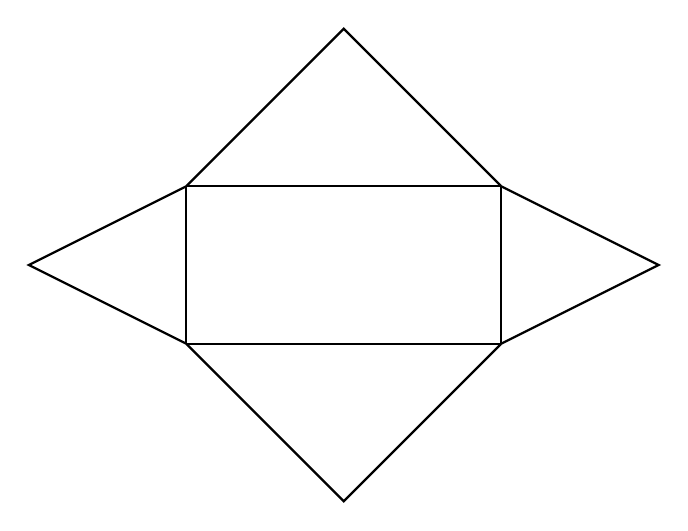
\begin{tikzpicture}[scale=1]

  \draw[thick] (0,0) -- (4,0); %SPODAJ
  \draw[thick] (4,0) -- (4,2); %DESNO
  \draw[thick] (4,2) -- (0,2); %ZGORAJ
  \draw[thick] (0,2) -- (0,0);%LEVO
  
  \draw[thick] (0,0) -- (2,-2) -- (4,0); %T-SPODAJ
  \draw[thick] (0,2) -- (2,4) -- (4,2); %T-ZGORAJ
  \draw[thick] (0,0) -- (-2,1) -- (0,2); %T-LEVO
  \draw[thick] (4,0) -- (6,1) -- (4,2); %T-DESNO

\end{tikzpicture}

\vspace{0.5em}
\textit{Mreža piramide s pravokotno osnovo \( a \times b \) in stranskimi robovi dolžine \( s \)}
\end{center}

}
\end{tabularx}

\razmak{0.5em}

% ******** 42. Stožec ********
\crta

\naslov{Stožec}

\begin{tabularx}{\textwidth}{X r}
\vprasanje{Opišite pokončni stožec.}{1 točka}
\odgovor{
\begin{itemize}
	\item Pokončni stožec je geometrijsko telo, ki nastane, ko točko (vrh stožca) povežemo z vsemi točkami osnovne ploskve (krožnica), pri čemer je vrh pravokotno nad središčem osnovne ploskve.
\end{itemize}
}
\end{tabularx}

\razmak{1em}

\begin{tabularx}{\textwidth}{X r}
\vprasanje{Narišite mrežo stožca.}{1 točka}
\odgovor{
\begin{itemize}
	\item Mreža stožca je sestavljena iz osnovne ploskve (krožnica) in odskega kroga, ki predstavlja plašč stožca.
\end{itemize}
}
\end{tabularx}

\begin{tabularx}{\textwidth}{X r}
\vprasanje{Opišite presek stožca z ravnino, ki vsebuje os stožca.}{1 točka}
\odgovor{
\begin{itemize}
	\item	Presek stožca z ravnino, ki vsebuje os stožca, je enakokrak trikotnik, katerega osnovnica je premer osnovne ploskve, stranici pa sta stranska robova stožca.
\end{itemize}
}
\end{tabularx}

\begin{tabularx}{\textwidth}{X r}
\vprasanje{Navedite formuli za izračun površine in prostornine pokončnega stožca.}{2 točki}
\odgovor{
\begin{itemize}
  \item Površina pokončnega stožca je vsota ploščine osnovne ploskve in plašča:
  \[
  P = \pi r^2 + \pi r s,
  \]
  kjer je $r$ polmer osnovne ploskve in $s$ poševna višina (stranska višina) stožca.
  \item Prostornina pokončnega stožca je:
  \[
  V = \frac{1}{3} \pi r^2 v,
  \]
  kjer je $v$ višina stožca.
\end{itemize}
}
\end{tabularx}

\begin{tabularx}{\textwidth}{X r}
\vprasanje{Izrazite višino enakostraničnega stožca s polmerom osnovne ploskve $r$.}{1 točka}
\odgovor{
\begin{itemize}
	\item Višina enakostraničnega stožca je izražena kot
	\[
	v = \sqrt{s^2 - r^2},
	\]
	kjer je $s$ dolžina poševne višine, ki je enaka stranskem robu enakostraničnega stožca. Pri enakostraničnem stožcu, kjer je osnovna ploskev krog in vsi robovi enaki, velja, da $s = 2r$, torej
	\[
	v = \sqrt{(2r)^2 - r^2} = r\sqrt{3}.
	\]
\end{itemize}
}
\end{tabularx}
\razmak{0.5em}


% ******** 43. Vekotrji ********
\crta

\naslov{Vekotrji}

\begin{tabularx}{\textwidth}{X r}
\vprasanje{Kaj je vektor?}{1 točka}
\odgovor{
\begin{itemize}
	\item Vektor je usmerjen daljica, ki jo določata smer, velikost (dolžina) in orientacija. Z njim ponazorimo premik iz ene točke v drugo.
\end{itemize}
}
\end{tabularx}

\begin{tabularx}{\textwidth}{X r}
\vprasanje{Definirajte seštevanje vektorjev.}{1 točka}
\odgovor{
\begin{itemize}
	\item Seštevanje vektorjev pomeni, da začetku drugega vektorja prislonimo konec prvega, rezultat pa je vektor od začetka prvega do konca drugega vektorja. Pomembno je da ohranimo smer, dolžino in orientacijo. Ni nujno, da je seštevek dveh vektorjev vzporeden vektorjema $\vec{a}$ ali $\vec{b}$.
\end{itemize}
}
\end{tabularx}

\begin{tabularx}{\textwidth}{X r}
\vprasanje{Definirajte ničelni vektor in nasprotni vektor danega vektorja.}{1 točka}
\odgovor{
\begin{itemize}
	\item Ničelni vektor je vektor z dolžino 0 in nima določene smeri. Označimo ga z $\vec{0}$. Nasprotni vektor danega vektorja ima enako dolžino, a nasprotno smer.
\end{itemize}
}
\end{tabularx}

\begin{tabularx}{\textwidth}{X r}
\vprasanje{Definirajte odštevanje vektorjev.}{1 točka}
\odgovor{
\begin{itemize}
	\item Odštevanje vektorjev $\vec{a} - \vec{b}$ je enako seštevku vektorja $\vec{a}$ in nasprotnega vektorja $-\vec{b}$: $\vec{a} - \vec{b} = \vec{a} + (-\vec{b})$.
\end{itemize}
}
\end{tabularx}

\begin{tabularx}{\textwidth}{X r}
\vprasanje{Povejte dve lastnosti seštevanja vektorjev.}{2 točka}
\odgovor{
\begin{itemize}
  \item \textbf{Komutativnost}: $\vec{a} + \vec{b} = \vec{b} + \vec{a}$.
  \item \textbf{Asociativnost}: $(\vec{a} + \vec{b}) + \vec{c} = \vec{a} + (\vec{b} + \vec{c})$.
\end{itemize}
}
\end{tabularx}

\razmak{0.5em}


% ******** 44. Vekotrji ********
\crta

\naslov{Vekotrji}

\begin{tabularx}{\textwidth}{X r}
\vprasanje{Definirajte množenje vektorja s skalarjem.}{1 točka}
\odgovor{
\begin{itemize}
	\item Množenje vektorja s skalarjem pomeni, da vektor pomnožimo s številom, kar spremeni njegovo dolžino in lahko tudi smer, če je skalar negativen.
	\item \textbf{Primer: } Naj bo $\vec{a} = (4, 1, 2)$, in skalar $k = 2$
	
	Potem: 
	\[
	k\vec{a} = (4k, 1k, 2k) = (8, 2, 4)
	\]
\end{itemize}
}
\end{tabularx}

\begin{tabularx}{\textwidth}{X r}
\vprasanje{Kaj je enotski vektor?}{1 točka}
\odgovor{
\begin{itemize}
	\item Enotski vektor je vektor, ki ima dolžino (normo) enako 1. Označuje le smer.
\end{itemize}
}
\end{tabularx}

\begin{tabularx}{\textwidth}{X r}
\vprasanje{Kakšna zveza velja med dvema neničelnima vzporednima vektorjema $\bar{a}$ in $\bar{b}$ ?}{1 točka}
\odgovor{
\begin{itemize}
	\item Če sta vektorja $\vec{a}$ in $\vec{b}$ vzporedna, potem obstaja skalar $k \in \mathbb{R} \setminus \{0\}$, da velja $\vec{a} = k\vec{b}$.
\end{itemize}
}
\end{tabularx}

\begin{tabularx}{\textwidth}{X r}
\multicolumn{2}{X}{
\textbf{\roman{vprasanje}.} 
%
% Macro za vpr je geeked...zato delam manual
%
\textbf{V pravilnem šestkotniku $ABCDEF$ s $S$ označimo presečišče najdaljših diagonal. 
Med vektorji $\overrightarrow{AB}, \overrightarrow{AD}, \overrightarrow{EF}, \overrightarrow{BC}$ in $\overrightarrow{SE}$ poiščite:} \begin{itemize}
  \item vse vzporedne vektorje \hfill (1 točka)
  \item par nasprotnih vektorjev \hfill (1 točka)
  \item par nekolinearnih vektorjev \hfill (1 točka)
\end{itemize}
} \\[0.5em]
\odgovor{
\begin{itemize}
  \item Vzporedni vektorji: $\overrightarrow{AD} \parallel \overrightarrow{EF}$, $\overrightarrow{EF} \parallel \overrightarrow{BC}$
  \item Nasprotna vektorja: $\overrightarrow{BC}$ in $\overrightarrow{EF}$
  \item Nekolinearna vektorja: $\overrightarrow{AB}$ in $\overrightarrow{AD}$
\end{itemize}
}
\stepcounter{vprasanje}
\end{tabularx}


% ******** 45. Vekotrji ********
\crta

\naslov{Vekotrji}

\begin{tabularx}{\textwidth}{X r}
\vprasanje{Opišite pravokotni koordinatni sistem v prostoru $\mathbb{R}^3$.}{1 točka}
\odgovor{
\begin{itemize}
  \item Pravokotni koordinatni sistem v $\mathbb{R}^3$ določajo tri med seboj pravokotne koordinatne osi: $x$ (abcisna os), $y$ (ordinatna os) in $z$ (aplikatna os).
  \item Vsaka točka v prostoru je določena z urejeno trojico realnih števil $(x, y, z)$.
  \item Izhodišče je točka, kjer se vse tri osi sekajo, označimo jo z $O(0, 0, 0)$.
\end{itemize}
}
\end{tabularx}

\begin{tabularx}{\textwidth}{X r}
\vprasanje{Definirajte standardno ortonormirano bazo v prostoru $\mathbb{R}^3$.}{1 točka}
\odgovor{
\begin{itemize}
  \item Standardna ortonormirana baza v $\mathbb{R}^3$ je množica treh med seboj pravokotnih enotskih vektorjev.
  \item Ta baza je: $\vec{i} = (1, 0, 0)$, $\vec{j} = (0, 1, 0)$, $\vec{k} = (0, 0, 1)$.
\end{itemize}
}
\end{tabularx}

\begin{tabularx}{\textwidth}{X r}
\vprasanje{Definirajte krajevni vektor dane točke v prostoru $\mathbb{R}^3$.}{1 točka}
\odgovor{
\begin{itemize}
  \item Krajevni vektor točke $A(a_1, a_2, a_3)$ je vektor, ki ima začetek v izhodišču $O(0, 0, 0)$ in konec v točki $A$.
  \item Označimo ga z $\vec{r}_A = \overrightarrow{OA}$ in ima komponente $(a_1, a_2, a_3)$.
\end{itemize}
}
\end{tabularx}

\begin{tabularx}{\textwidth}{X r}
\vprasanje{Izrazite krajevni vektor $r_{\mathrm{A}}$ točke $A\left(a_1, a_2, a_3\right)$ kot linearno kombinacijo vektorjev standardne ortonormirane baze prostora $\mathbb{R}^3$.}{1 točka}
\odgovor{
\begin{itemize}
  \item Krajevni vektor $\vec{\tau}_A = a_1 \vec{i} + a_2 \vec{j} + a_3 \vec{k}$.
  \item To pomeni, da vektor izrazimo kot linearno kombinacijo enotskih vektorjev baze $\vec{i}, \vec{j}, \vec{k}$.
\end{itemize}
}
\end{tabularx}

\begin{tabularx}{\textwidth}{X r}
\vprasanje{Naj bosta $A$ in $B$ točki v prostoru $\mathbb{R}^3$. Izrazite vektor $\overrightarrow{AB}$ s koordinatami točk $A$ in $B$ in odgovor utemejite.}{2 točki}
\odgovor{
\begin{itemize}
  \item Naj bo $A(a_1, a_2, a_3)$ in $B(b_1, b_2, b_3)$. Vektor $\overrightarrow{AB}$ ima koordinate $(b_1 - a_1,\ b_2 - a_2,\ b_3 - a_3)$.
  \item Utemeljitev: Vektor $\overrightarrow{AB}$ dobimo tako, da od krajevnega vektorja točke $B$ odštejemo krajevni vektor točke $A$: $\vec{r}_B - \vec{r}_A$.
\end{itemize}
}
\end{tabularx}

\razmak{0.5em}


% ******** 46. Skalarni produkt ********
\crta

\naslov{Skalarni produkt}

\begin{tabularx}{\textwidth}{X r}
\vprasanje{Kako izračunamo skalarni produkt dveh vektorjev, če poznamo njuni dolžini in kot med njima?}{1 točka}
\odgovor{
\begin{itemize}
  \item Skalarni produkt dveh vektorjev $\vec{a}$ in $\vec{b}$ je enak: $\vec{a} \cdot \vec{b} = |\vec{a}| \cdot |\vec{b}| \cdot \cos \varphi$, kjer je $\varphi$ kot med vektorjema.
\end{itemize}
}
\end{tabularx}

\begin{tabularx}{\textwidth}{X r}
\vprasanje{Naštejte dve lastnosti skalarnega produkta.}{2 točki}
\odgovor{
\begin{itemize}
  \item \textbf{Komutativnost}: $\vec{a} \cdot \vec{b} = \vec{b} \cdot \vec{a}$.
  \item \textbf{Distributivnost glede na seštevanje}: $\vec{a} \cdot (\vec{b} + \vec{c}) = \vec{a} \cdot \vec{b} + \vec{a} \cdot \vec{c}$.
\end{itemize}
}
\end{tabularx}

\begin{tabularx}{\textwidth}{X r}
\vprasanje{Kako s skalarnim produktom ugotovimo, ali sta dana vektorja pravokotna? Pokažite s primerom.}{2 točka}
\odgovor{
\begin{itemize}
  \item Dva vektorja sta pravokotna, če je njun skalarni produkt enak $0$: $\vec{a} \cdot \vec{b} = 0$.
  \item Primer: naj bo $\vec{a} = (1, 2)$ in $\vec{b} = (2, -1)$. Potem je $\vec{a} \cdot \vec{b} = 1 \cdot 2 + 2 \cdot (-1) = 2 - 2 = 0$, torej sta vektorja pravokotna.
\end{itemize}
}
\end{tabularx}

\begin{tabularx}{\textwidth}{X r}
\vprasanje{Izračunajte $\vec{a} \cdot \vec{a}$ in razložite dobljeno zvezo.}{1 točka}
\odgovor{
\begin{itemize}
  \item Skalarni produkt $\vec{a} \cdot \vec{a} = |\vec{a}|^2$, torej kvadrat dolžine vektorja.
  \item Primer: če je $\vec{a} = (3, 4)$, potem $\vec{a} \cdot \vec{a} = 3^2 + 4^2 = 9 + 16 = 25$, kar je $|\vec{a}|^2 = 5^2$.
\end{itemize}
}
\end{tabularx}

\razmak{0.5em}


% ******** 47. Skalarni produkt v standardni ortonormirani bazi ********
\crta

\naslov{Skalarni produkt v standardni ortonormirani bazi}

\begin{tabularx}{\textwidth}{X r}
\vprasanje{Kako izračunamo skalarni produkt dveh vektorjev v standardni ortonormirani bazi?}{1 točka}
\odgovor{
\begin{itemize}
  \item Naj bosta $\vec{a} = (a_1, a_2, a_3)$ in $\vec{b} = (b_1, b_2, b_3)$. Potem je skalarni produkt: 
  \[
  \vec{a} \cdot \vec{b} = a_1 b_1 + a_2 b_2 + a_3 b_3.
  \]
\end{itemize}
}
\end{tabularx}

\begin{tabularx}{\textwidth}{X r}
\vprasanje{Kako izračunamo dolžino vektorja v standardni ortonormirani bazi? Odgovor utemeljite.}{2 točki}
\odgovor{
\begin{itemize}
  \item Naj bo $\vec{a} = (a_1, a_2, a_3)$. Dolžino vektorja izračunamo po formuli:
  \[
  |\vec{a}| = \sqrt{a_1^2 + a_2^2 + a_3^2}.
  \]
  \item Utemeljitev: To sledi iz Pitagorovega izreka v prostoru, saj standardna ortonormirana baza pomeni, da so bazni vektorji med seboj pravokotni in enotni po dolžini.
\end{itemize}
}
\end{tabularx}

\begin{tabularx}{\textwidth}{X r}
\vprasanje{Kako izračunamo kot med vektorjema v standardni ortonormirani bazi?}{1 točka}
\odgovor{
\begin{itemize}
  \item Kot $\varphi$ med vektorjema $\vec{a}$ in $\vec{b}$ dobimo iz formule:
  \[
  \cos \varphi = \frac{\vec{a} \cdot \vec{b}}{|\vec{a}| \cdot |\vec{b}|}.
  \]
  \item Nato kot izračunamo z inverzno funkcijo: $\varphi = \arccos\left( \frac{\vec{a} \cdot \vec{b}}{|\vec{a}| \cdot |\vec{b}|} \right)$.
\end{itemize}
}
\end{tabularx}

\begin{tabularx}{\textwidth}{X r}
\vprasanje{Ponazorite izračun kota med vektorjema s primerom.}{2 točki}
\odgovor{
\begin{itemize}
  \item Naj bosta $\vec{a} = (1, 2, 2)$ in $\vec{b} = (2, 0, 1)$.
  \item Skalarni produkt: $\vec{a} \cdot \vec{b} = 1 \cdot 2 + 2 \cdot 0 + 2 \cdot 1 = 2 + 0 + 2 = 4$.
  \item Dolžini: $|\vec{a}| = \sqrt{1^2 + 2^2 + 2^2} = \sqrt{9} = 3$, $|\vec{b}| = \sqrt{2^2 + 0^2 + 1^2} = \sqrt{5}$.
  \item Kot: 
  \[
  \cos \varphi = \frac{4}{3 \cdot \sqrt{5}}, \quad \varphi = \arccos\left(\frac{4}{3\sqrt{5}}\right) \approx 70.402^\circ.
  \]
\end{itemize}
}
\end{tabularx}

\razmak{0.5em}


% ******** 48. Koordniatni sistem v ravnini ********
\crta

\naslov{Koordniatni sistem v ravnini}

\begin{tabularx}{\textwidth}{X r}
\vprasanje{Opišite pravokotni koordinatni sistem v ravnini $\mathbb{R}^2$.}{1 točka}
\odgovor{
\begin{itemize}
  \item Pravokotni koordinatni sistem v ravnini $\mathbb{R}^2$ sestavljata dve med seboj pravokotni premici: abscisna os ($x$-os) in ordinatna os ($y$-os), ki se sekata v koordinatnem izhodišču.
  \item Vsaka točka v ravnini je določena z urejenim parom $(x, y)$, kjer je $x$ razdalja od ordinatne osi, $y$ pa od abscisne osi.
\end{itemize}
}
\end{tabularx}

\begin{tabularx}{\textwidth}{X r}
\vprasanje{Izpeljite formulo za računanje razdalje med dvema točkama.}{2 točki}
\odgovor{
\begin{itemize}
  \item Naj bosta dani točki $A(x_1, y_1)$ in $B(x_2, y_2)$.
  \item Razdaljo med njima dobimo s Pitagorovim izrekom:
  \[
  |AB| = \sqrt{(x_2 - x_1)^2 + (y_2 - y_1)^2}.
  \]
\end{itemize}
}
\end{tabularx}

\begin{tabularx}{\textwidth}{X r}
\vprasanje{Povejte koordinati razpolovišča daljice z danima krajiščema.}{1 točka}
\odgovor{
\begin{itemize}
  \item Naj bosta krajišči $A(x_1, y_1)$ in $B(x_2, y_2)$.
  \item Koordinati razpolovišča $S$ sta:
  \[
  S = \left( \frac{x_1 + x_2}{2}, \frac{y_1 + y_2}{2} \right).
  \]
\end{itemize}
}
\end{tabularx}

\razmak{1em}

\begin{tabularx}{\textwidth}{X r}
\vprasanje{Točko $T(x, y)$ prezrcalite čez koordinatno izhodišče. Povejte koordinati tako dobljene točke.}{1 točka}
\odgovor{
\begin{itemize}
  \item Prezrcaljena točka ima koordinati:
  \[
  T' = (-x, -y).
  \]
\end{itemize}
}
\end{tabularx}

\begin{tabularx}{\textwidth}{X r}
\vprasanje{Točko $T(x, y)$ prezrcalite čez ordinatno os. Povejte koordinati tako dobljene točke.}{1 točka}
\odgovor{
\begin{itemize}
  \item Prezrcaljena točka ima koordinati:
  \[
  T' = (-x, y).
  \]
\end{itemize}
}
\end{tabularx}

\razmak{0.5em}


% ******** 49. Funkcije ********
\crta

\naslov{Funkcije}

\begin{tabularx}{\textwidth}{X r}
\vprasanje{Definirajte pojem funkcije (preslikave) iz množice $A$ v množico $B$.}{1 točka}
\odgovor{
\begin{itemize}
  \item Funkcija (ali preslikava) $f$ iz množice $A$ v množico $B$ je pravilo, ki vsakemu elementu $a \in A$ priredi natanko en element $b \in B$, torej $f: A \to B$.
\end{itemize}
}
\end{tabularx}

\begin{tabularx}{\textwidth}{X r}
\vprasanje{Definirajte pojme definicijsko območje, zaloga vrednosti in graf funkcije.}{3 točke}
\odgovor{
\begin{itemize}
  \item \textbf{Definicijsko območje} funkcije je množica vseh tistih vrednosti $x$, za katere je funkcija $f(x)$ definirana.
  \item \textbf{Zaloga vrednosti} funkcije je množica vseh možnih vrednosti $f(x)$.
  \item \textbf{Graf funkcije} je množica točk v ravnini, ki imajo koordinate oblike $(x, f(x))$, kjer $x$ teče po definicijskem območju.
\end{itemize}
}
\end{tabularx}

\begin{tabularx}{\textwidth}{X r}
\vprasanje{Narišite graf ali povejte predpis funkcije $f$, ki ima zalogo vrednosti $Z_f=(2, \infty)$.}{1 točka}
\odgovor{
\begin{itemize}
  \item Primer funkcije: $f(x) = \mathrm{e}^x + 2$.
  \item Zaloga vrednosti te funkcije je $Z_f = (2, \infty)$.
\end{itemize}
}
\end{tabularx}

\begin{tabularx}{\textwidth}{X r}
\vprasanje{Narišite graf ali povejte predpis funkcije $g$, ki ima definicijsko območje $D_s=(2, \infty)$.}{1 točka}
\odgovor{
\begin{itemize}
  \item Primer funkcije: $g(x) = \ln(x - 2)$.
  \item Definicijsko območje te funkcije je $D_s = (2, \infty)$.
\end{itemize}
}
\end{tabularx}

\razmak{0.5em}


% ******** 50. Lastnosti funkcij ********
\crta

\naslov{Lastnosti funkcij}

\begin{tabularx}{\textwidth}{X r}
\vprasanje{Kdaj je funkcija na intervalu narašajoča in kdaj padajoča?}{2 točki}
\odgovor{
\begin{itemize}
  \item Funkcija $f$ je na intervalu \textbf{naraščajoča}, če za vsak $x_1 < x_2$ v tem intervalu velja $f(x_1) \leq f(x_2)$.
  \item Funkcija $f$ je na intervalu \textbf{strogo naraščajoča}, če velja $f(x_1) < f(x_2)$ za vsak $x_1 < x_2$.
  \item Funkcija $f$ je na intervalu \textbf{padajoča}, če za vsak $x_1 < x_2$ v tem intervalu velja $f(x_1) \geq f(x_2)$.
  \item Funkcija $f$ je na intervalu \textbf{strogo padajoča}, če velja $f(x_1) > f(x_2)$ za vsak $x_1 < x_2$.
\end{itemize}
}
\end{tabularx}

\begin{tabularx}{\textwidth}{X r}
\vprasanje{Narišite graf ali povejte predpis funkcije, ki ni niti narašajoča niti padajoča.}{1 točka}
\odgovor{
\begin{itemize}
  \item Primer funkcije: $f(x) = \sin x$.
  \item Ta funkcija izmenično narašča in pada, zato ni niti naraščajoča niti padajoča v celoti. Naraščajoča: $(0, \frac{\pi}{2})$, padajoča $(\frac{\pi}{2}, \pi)$.
\end{itemize}
}
\end{tabularx}

\begin{tabularx}{\textwidth}{X r}
\vprasanje{Kdaj je funkcija $f$ omejena?}{2 točki}
\odgovor{
\begin{itemize}
  \item Funkcija $f$ je \textbf{omejena navzgor}, če obstaja realno število $M$, da za vsak $x$ v njenem definicijskem območju velja $f(x) \leq M$.
  \item Funkcija $f$ je \textbf{omejena navzdol}, če obstaja realno število $m$, da za vsak $x$ v njenem definicijskem območju velja $f(x) \geq m$.
  \item Funkcija $f$ je \textbf{omejena}, če obstajata realni števili $m$ in $M$, da za vsak $x$ velja $m \leq f(x) \leq M$.
\end{itemize}
}
\end{tabularx}

\begin{tabularx}{\textwidth}{X r}
\vprasanje{Narišite graf ali povejte predpis padajoče funkcije, ki je navzgor omejena, navzdol pa neomejena.}{1 točka}
\odgovor{
\begin{itemize}
  \item Primer funkcije: $f(x) = -\mathrm{e}^x$.
  \item Ta funkcija je strogo padajoča, njena največja vrednost je $f(x) \to 0$ (ko $x \to -\infty$), zato je navzgor omejena.
  \item Navzdol pa ni omejena, saj $f(x) \to -\infty$ (ko $x \to \infty$).
\end{itemize}
}
\end{tabularx}

\razmak{0.5em}


% ******** 51. Lastnosti funkcij ********
\crta

\naslov{Lastnosti funkcij}

\begin{tabularx}{\textwidth}{X r}
\vprasanje{Kdaj je funkcija $f$ liha in kdaj soda?}{2 točki}
\odgovor{
\begin{itemize}
  \item Funkcija $f$ je \textbf{soda}, če za vsak $x$ iz definicijskega območja velja: $f(-x) = f(x)$.
  \item Funkcija $f$ je \textbf{liha}, če za vsak $x$ iz definicijskega območja velja: $f(-x) = -f(x)$.
\end{itemize}
}
\end{tabularx}

\begin{tabularx}{\textwidth}{X r}
\vprasanje{Kako iz grafa funkcije $f$ vidimo, ali je funkcija $f$ soda oziroma liha?}{2 točki}
\odgovor{
\begin{itemize}
  \item Funkcija $f$ je \textbf{soda}, če je njen graf simetričen glede na ordinatno os (os $y$).
  \item Funkcija $f$ je \textbf{liha}, če je njen graf simetričen glede na koordinatno izhodišče.
\end{itemize}
}
\end{tabularx}

\begin{tabularx}{\textwidth}{X r}
\vprasanje{Naj bo funkcija $f$ bijektivna. Kako poišemo predpis inverzne funkcije $f^{-1}$ ?}{1 točka}
\odgovor{
\begin{itemize}
  \item Zapišemo enačbo $y = f(x)$.
  \item Zamenjamo vlogi $x$ in $y$: $x = f(y)$.
  \item Izražamo $y$ iz dobljene enačbe, tako dobimo $f^{-1}(x)$.
\end{itemize}
}
\end{tabularx}

\begin{tabularx}{\textwidth}{X r}
\vprasanje{Kaj velja za grafa funkcij $f$ in $f^{-1}$ ?}{1 točka}
\odgovor{
\begin{itemize}
  \item Graf funkcije $f^{-1}$ je simetričen z grafom funkcije $f$ glede na premico $y = x$ (simetrala lihih kvadrantov).
\end{itemize}
}
\end{tabularx}

\razmak{0.5em}


% ******** 52. Linearna funkcija ********
\crta

\naslov{Linearna funkcija}

\begin{tabularx}{\textwidth}{X r}
\vprasanje{Definirajte linearno funkcijo in povejte, kaj je njen graf.}{2 točki}
\odgovor{
\begin{itemize}
  \item Linearna funkcija je funkcija oblike $f(x) = kx + n$, kjer sta $k$ in $n$ realni števili ($k, n \in \mathbb{R}$).
  \item Graf linearne funkcije je premica.
\end{itemize}
}
\end{tabularx}

\begin{tabularx}{\textwidth}{X r}
\vprasanje{V odvisnosti od diferenčnega količnika $k$ preučite naraščanje in padanje linearne funkcije $f$.}{2 točki}
\odgovor{
\begin{itemize}
  \item Če je $k > 0$, je funkcija \textbf{naraščajoča}.
  \item Če je $k < 0$, je funkcija \textbf{padajoča}.
  \item Če je $k = 0$, je funkcija \textbf{konstantna}.
\end{itemize}
}
\end{tabularx}

\begin{tabularx}{\textwidth}{X r}
\vprasanje{Za koliko se spremeni vrednost funkcije $f$, če vrednost neodvisne spremenljivke povečamo za 2?}{1 točka}
\odgovor{
\begin{itemize}
  \item Vrednost funkcije se poveča za $2k$, kjer je $k$ smerni koeficient linearne funkcije.
\end{itemize}
}
\end{tabularx}

\begin{tabularx}{\textwidth}{X r}
\vprasanje{Kaj velja za grafa linearnih funkcij z enakima smernima koeficientoma?}{1 točka}
\odgovor{
\begin{itemize}
  \item Grafa sta par \textbf{vzporednih premic}.
\end{itemize}
}
\end{tabularx}

\razmak{0.5em}


% ******** 53. Enačba premice ********
\crta

\naslov{Enačba premice}

\begin{tabularx}{\textwidth}{X r}
\vprasanje{Zapišite eksplicitno obliko enačbe premice. Enačbe katerih premic lahko zapišemo v tej obliki?}{2 točki}
\odgovor{
\begin{itemize}
  \item Eksplicitna oblika enačbe premice je
  \[
  y = kx + n
  \]
  kjer je $k$ smerni koeficient in $n$ začetna vrednost.
  \item V tej obliki lahko zapišemo enačbe vseh premic, ki \textbf{niso navpične} (to pomeni, da imajo določen $k$).
\end{itemize}
}
\end{tabularx}

\begin{tabularx}{\textwidth}{X r}
\vprasanje{Zapišite implicitno obliko enačbe premice. Enačbe katerih premic lahko zapišemo v tej obliki?}{2 točki}
\odgovor{
\begin{itemize}
  \item Implicitna oblika enačbe premice je
  \[
  ax + by + c = 0
  \]
  
  kjer $a$, $b$ in $c$ pripadajo množici realnih števil.
  \item V tej obliki lahko zapišemo \textbf{enačbo vsake premice} v ravnini $\mathbb{R}^2$ (vključno z vodoravnimi in navpičnimi).
\end{itemize}
}
\end{tabularx}

\begin{tabularx}{\textwidth}{X r}
\vprasanje{Zapišite odsekovno obliko enačbe premice. Enačbe katerih premic lahko zapišemo v tej obliki?}{2 točki}
\odgovor{
\begin{itemize}
  \item Odsekovna oblika enačbe premice je 
  \[
  \frac{x}{a} + \frac{y}{b} = 1
  \]
  kjer $a$ in $b$ sta realni števili različni od $0$.
  \item V tej obliki lahko zapišemo enačbe vseh premic, ki \textbf{presekata koordinatni osi} (torej ne smejo biti vzporedne nobeni od obeh osi).
\end{itemize}
}
\end{tabularx}

\razmak{0.5em}

% ******** 54. Premice v ravnini ********
\crta

\naslov{Premice v ravnini}

\begin{tabularx}{\textwidth}{X r}
\vprasanje{Definirajte naklonski kot premice v ravnini ter razložite zvezo med naklonskim kotom in smernim koeficientom dane premice (če ta obstaja).}{2 točki}
\odgovor{
\begin{itemize}
  \item Naklonski kot $\varphi$ premice je orientirani kot med pozitivno smerjo osi $x$ in premico.
  \item Če premica ni navpična, ima smerni koeficient $k$ in velja zveza $\tan(\varphi) = k$.
\end{itemize}
}
\end{tabularx}

\begin{tabularx}{\textwidth}{X r}
\vprasanje{Kako izračunamo kot med premicama, če poznamo njuna smerna koeficienta?}{1 točka}
\odgovor{
\begin{itemize}
  \item Če sta $k_1$ in $k_2$ smerna koeficienta, potem kot $\alpha$ med premicama izračunamo z:
  \[
  \tan(\alpha) = \left| \frac{k_2 - k_1}{1 + k_1 k_2} \right|
  \]
\end{itemize}
}
\end{tabularx}

\begin{tabularx}{\textwidth}{X r}
\vprasanje{Kaj velja za smerna koeficienta vzporednih premic?}{1 točka}
\odgovor{
\begin{itemize}
  \item Premici sta vzporedni, če imata enaka smerna koeficienta: $k_1 = k_2$.
\end{itemize}
}
\end{tabularx}

\begin{tabularx}{\textwidth}{X r}
\vprasanje{Kaj velja za smerna koeficienta pravokotnih premic?}{1 točka}
\odgovor{
\begin{itemize}
  \item Premici sta pravokotni, če je produkt njunih smernih koeficientov $k_1 \cdot k_2 = -1$.
\end{itemize}
}
\end{tabularx}

\begin{tabularx}{\textwidth}{X r}
\vprasanje{Kolikšen je smerni koeficient premice, ki je pravokotna na simetralo lihih kvadrantov?}{1 točka}
\odgovor{
\begin{itemize}
  \item Simetrala lihih kvadrantov ima enačbo $y = x$, torej $k = 1$.
  \item Premica, pravokotna nanjo, ima smerni koeficient $k = -1$.
\end{itemize}
}
\end{tabularx}

\razmak{0.5em}


% ******** 55. Linearne neenačbe ********
\crta

\naslov{Linearne neenačbe}

\begin{tabularx}{\textwidth}{X r}
\vprasanje{Kaj je linearna neenačba z eno neznanko?}{1 točka}
\odgovor{
\begin{itemize}
	\item Linearna neenačba z eno neznanko je neenačba oblike $ax + b \, \square \, 0$, kjer je $a \neq 0$, $b \in \mathbb{R}$, $x$ je neznanka, $\square$ pa je eden izmed simbolov $<$, $>$, $\leq$, $\geq$.
\end{itemize}
}
\end{tabularx}

\begin{tabularx}{\textwidth}{X r}
\vprasanje{Na primeru opišite reševanje linearnih neenačb z eno neznanko.}{2 točki}
\odgovor{
\begin{itemize}
	\item Primer: $3x - 5 < 7$
	\[
	\begin{array}{rcl}
		3x - 5 &< &7 \\
		3x &< &12 \\
		x &< &4
	\end{array}
	\]
\end{itemize}
Rešitev je množica vseh realnih števil, manjših od 4: $\{x \in \mathbb{R} \mid x < 4\}$.
}
\end{tabularx}

\razmak{1em}

\begin{tabularx}{\textwidth}{X r}
\vprasanje{Opišite vse možne množice rešitev poljubne linearne neenačbe z eno neznanko.}{3 točke}
\odgovor{
\begin{itemize}
	\item Rešitev linearne neenačbe z eno neznanko je lahko:
	\begin{itemize}
	  \item Interval neskončno mnogo rešitev (npr. $x > 2$, rešitev: $(2, \infty)$).
	  \item Množica realnih števil (npr. $2x + 3 > 2x - 1$, rešitev: $\mathbb{R}$).
	  \item Brez rešitve (npr. $3x + 1 < 3x - 2$, rešitev: $\emptyset$ oz. $\{\}$).
	\end{itemize}
\end{itemize}
}
\end{tabularx}

\razmak{0.5em}


% ******** 56. Potenčna funkcija ********
\crta

\naslov{Potenčna funkcija}

\begin{tabularx}{\textwidth}{X r}
\vprasanje{Definirajte potenčno funkcijo z naravnim eksponentom.}{1 točka}
\odgovor{
\begin{itemize}
	\item Potenčna funkcija z naravnim eksponentom je funkcija oblike $f(x) = x^n$, kjer je $n \in \mathbb{N}$.
\end{itemize}
}
\end{tabularx}

\begin{tabularx}{\textwidth}{X r} 
\vprasanje{Narišite grafa potenčnih funkcij, ki imata eksponenta 2 in 3.}{2 točki}
\odgovor{
\begin{itemize}
	\item Funkcija $f(x) = x^2$: parabola, simetrična glede na ordinatno os ($y$), minimum v točki $(0, 0)$. 
	\item Funkcija $g(x) = x^3$: krivulja, simetrična glede na izhodišče, naraščujoča od $(-\infty, \infty)$.
\end{itemize}

\centering
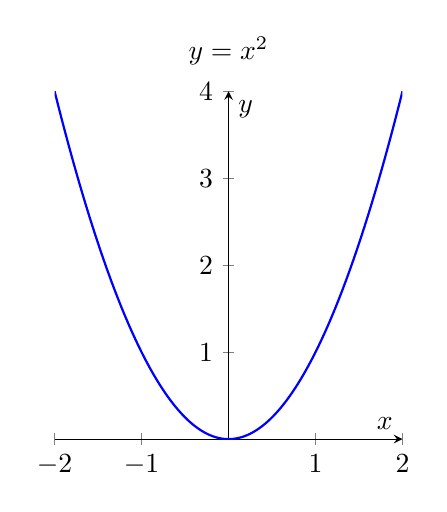
\begin{tikzpicture}
  \begin{axis}[
    title={$y = x^2$},
    axis lines=middle,
    xlabel=$x$, ylabel=$y$,
    domain=-2:2,
    samples=100,
    width=6cm, height=6cm,
  ]
    \addplot[blue, thick] {x^2};
  \end{axis}
\end{tikzpicture}
\quad
\begin{tikzpicture}
  \begin{axis}[
    title={$y = x^3$},
    axis lines=middle,
    xlabel=$x$, ylabel=$y$,
    domain=-2:2,
    samples=100,
    width=6cm, height=6cm,
  ]
    \addplot[red, thick] {x^3};
  \end{axis}
\end{tikzpicture}

}
\end{tabularx}

\begin{center}
\small{Grafi funkcij $y=x^2$ in $y=x^3$}
\end{center}


\begin{tabularx}{\textwidth}{X r}
\vprasanje{Navedite vsaj dve lastnosti potenčnih funkcij.}{1 točka}
\odgovor{
\begin{itemize}
  \item So zvezne in definirane za vsak $n$, kjer $n \in \mathbb{R}$.
  \item Za lih $n$ je funkcija liha in strogo monotona, za sod $n$ je soda in ima minimum v $(0, 0)$.
\end{itemize}
}
\end{tabularx}

\begin{tabularx}{\textwidth}{X r}
\vprasanje{Navedite osnovne razlike v lastnostih med potenčnimi funkcijami s sodim in potenčnimi funkcijami z lihim naravnim eksponentom.}{2 točki}
\odgovor{
\begin{itemize}
  \item Funkcija s sodim eksponentom ($n$ sodo) je \textbf{soda} funkcija (simetrična glede na $y$-os), ima minimum v $(0, 0)$ in je nenegativna.
  \item Funkcija z lihim eksponentom ($n$ liho) je \textbf{liha} funkcija (simetrična glede na izhodišče), njen graf poteka skozi vse kvadrante, je strogo rastoča.
\end{itemize}
}
\end{tabularx}

\razmak{0.5em}


% ******** 57. Korenska funkcija ********
\crta

\naslov{Korenska funkcija}

\begin{tabularx}{\textwidth}{X r}
\vprasanje{Za poljubno naravno število $n$ definirajte korensko funkcijo $f$ s predpisom $f(z)=\sqrt[n]{x}$.}{2 točki}
\odgovor{
\begin{itemize}
	\item Korenska funkcija s predpisom $f(x) = \sqrt[n]{x}$ za poljubno naravno število $n$ je inverzna funkcija potenčne funkcije $x^n$.
	\item Če je $n$ liho (npr. $n=3$), potem je $f(x) = \sqrt[3]{x}$ definirana za vsa realna števila $x$, njen graf je zvezna in liha funkcija.
	\item Funkcija $f(x) = \sqrt[3]{x}$ je strogo naraščajoča.
\end{itemize}
}
\end{tabularx}

\begin{tabularx}{\textwidth}{X r}
\vprasanje{Narišite grafa korenskih funkcij za $n=2$ in $n=3$.}{2 točki}
\odgovor{
\begin{itemize}
	\item Opis grafov:
	\begin{itemize}
  		\item $f(x) = \sqrt{x}$: definiran za $x \geq 0$, graf leži v prvem kvadrantu, narašča, ni linearen.
		\item $g(x) = \sqrt[3]{x}$: definiran za vsa realna $x$, graf poteka skozi izhodišče in je simetričen glede na izhodišče (liha funkcija).
	\end{itemize}
\end{itemize}

\centering
\begin{tikzpicture}
  \begin{axis}[
    title={$y = \sqrt{x}$},
    axis lines=middle,
    xlabel=$x$, ylabel=$y$,
    domain=0:4,
    samples=100,
    width=6cm, height=6cm,
  ]
    \addplot[blue, thick] {sqrt(x)};
  \end{axis}
\end{tikzpicture}
\quad
\begin{tikzpicture}
  \begin{axis}[
    title={$y = \sqrt[3]{x}$},
    axis lines=middle,
    xlabel=$x$, ylabel=$y$,
    domain=-4:4,
    samples=100,
    width=6cm, height=6cm,
  ]
    \addplot[red, thick] {x^(1/3)};
  \end{axis}
\end{tikzpicture}

}
\end{tabularx}

\begin{center}
\small{Grafi korenskih funkcij $y = \sqrt{x}$ in $y = \sqrt[3]{x}$}
\end{center}


\begin{tabularx}{\textwidth}{X r}
\vprasanje{Navedite definicijski območji in zalogi vrednosti korenskih funkcij za $n=2$ in $n=3$.}{2 točki}
\odgovor{
\begin{itemize}
	\item \textbf{Za $n = 2$ (kvadratni koren):}
	\begin{itemize}
	  \item Definicijsko območje: $D_f = [0, \infty)$
	  \item Zaloga vrednosti: $Z_f = [0, \infty)$
	\end{itemize}

	\item \textbf{Za $n = 3$ (kubični koren):}
	\begin{itemize}
	  \item Definicijsko območje: $D_g = \mathbb{R}$
	  \item Zaloga vrednosti: $Z_g = \mathbb{R}$
	\end{itemize}
\end{itemize}
}
\end{tabularx}

\razmak{0.5em}


% ******** 58. Kvadratna funkcija ********
\crta

\naslov{Kvadratna funkcija}

\begin{tabularx}{\textwidth}{X r}
\vprasanje{Definirajte kvadratno funkcijo.}{1 točka}
\odgovor{
\begin{itemize}
	\item Kvadratna funkcija je funkcija oblike $f(x) = ax^2 + bx + c$, kjer je $a \neq 0$ in $a$, $b$, $c$ realna števila. Graf funkcije je parabola.
\end{itemize}
}
\end{tabularx}

\begin{tabularx}{\textwidth}{X r}
\vprasanje{Naštejte vsaj štiri lastnosti kvadratne funkcije in jih razložite.}{4 točke}
\odgovor{
\begin{itemize}
  \item \textbf{Graf}: graf kvadratne funkcije je \textit{parabola}.
  \item \textbf{Odprtost}: če je $a > 0$, je parabola odprta navzgor; če je $a < 0$, je odprta navzdol.
  \item \textbf{Teme (vrh) parabole}: koordinati temena sta $p = -\frac{b}{2a}$ in $q = -\frac{D}{4a}$.
  \item \textbf{Os simetrije}: premica $x = -\frac{b}{2a}$ je os simetrije grafa.
  \item \textbf{Zaloga vrednosti}: če je $a > 0$, je zaloga $[\text{min}, \infty)$; če je $a < 0$, pa $(-\infty, \text{max}]$.
\end{itemize}
}
\end{tabularx}

\begin{tabularx}{\textwidth}{X r}
\vprasanje{Povejte primer navzgor omejene kvadratne funkcije, katere graf seka ordinatno os $v$ točki $N(0,3)$.}{1 točka}
\odgovor{
\begin{itemize}
	\item Primer take funkcije je $f(x) = -x^2 + 2x + 3$. Ker je $a = -1 < 0$, je funkcija navzgor omejena. Za $x = 0$ je $f(0) = 3$, torej graf seka ordinatno os v točki $N(0, 3)$.
\end{itemize}
}
\end{tabularx}
\razmak{0.5em}


% ******** 59. Teme grafa kvadratne funkcije ********
\crta

\naslov{Teme grafa kvadratne funkcije}

\begin{tabularx}{\textwidth}{X r}
\vprasanje{Kaj je teme grafa kvadratne funkcije? Kako ga izračunamo?}{2 točki}
\odgovor{
\begin{itemize}
  \item Teme grafa kvadratne funkcije je najvišja ali najnižja točka grafa (parabole), odvisno od tega, ali je parabola odprta navzgor ali navzdol.
  \item Koordinati temena funkcije $f(x) = ax^2 + bx + c$ izračunamo po obrazcu:
  \[
  x = -\frac{b}{2a}, \quad y = -\frac{D}{4a}, \text{kjer je } D  = b^2 -4ac
  \]
\end{itemize}
}
\end{tabularx}

\begin{tabularx}{\textwidth}{X r}
\vprasanje{Povejte temensko obliko predpisa kvadratne funkcije. Kako je njen graf odvisen od vodilnega koeficienta ter koordinat temena?}{3 točk3}
\odgovor{
\begin{itemize}
  \item Temenska oblika kvadratne funkcije je: 
  \[
  f(x) = a(x - p)^2 + q
  \]
  kjer je $(p, q)$ teme parabole.
  \item Parameter $a$ določa:
  \begin{itemize}
    \item smer odprtosti (če je $a > 0$, je parabola odprta navzgor, konveksna; če je $a < 0$, navzdol, konkavna),
    \item širino parabole (večja kot je absolutna vrednost $|a|$ ožja je parabola).
  \end{itemize}
  \item Koordinati $(p, q)$ določata lego temena in s tem tudi lego celotne parabole v koordinatnem sistemu.
\end{itemize}
}
\end{tabularx}

\begin{tabularx}{\textwidth}{X r}
\vprasanje{Povejte primer navzgor omejene kvadratne funkcije, katere graf ima teme v prvem kvadrantu.}{1 točka}
\odgovor{
\begin{itemize}
  \item Primer take funkcije je: 
  \[
  f(x) = -2(x - 1)^2 + 3
  \]
  \item Graf ima teme v točki $(1, 3)$, ki leži v prvem kvadrantu, in ker je $a = -2 < 0$, je funkcija navzgor omejena.
\end{itemize}
}
\end{tabularx}

\razmak{0.5em}


% ******** 60. Ničle kvadratne funkcije ********
\crta

\naslov{Ničle kvadratne funkcije}

\begin{tabularx}{\textwidth}{X r}
\vprasanje{Definirajte ničlo funkcije.}{1 točka}
\odgovor{
\begin{itemize}
  \item Ničla funkcije je vrednost spremenljivke $x$, pri kateri je vrednost funkcije enaka 0:
  \[
  f(x) = 0
  \]
  \item To pomeni, da graf funkcije seka abcisno os (os $x$) v tej točki.
\end{itemize}
}
\end{tabularx}

\begin{tabularx}{\textwidth}{X r}
\vprasanje{Povejte ničelno obliko predpisa kvadratne funkcije.}{1 točka}
\odgovor{
\begin{itemize}
  \item Ničelna oblika kvadratne funkcije je:
  \[
  f(x) = a(x - x_1)(x - x_2)
  \]
  \item kjer sta $x_1$ in $x_2$ ničli funkcije.
\end{itemize}
}
\end{tabularx}

\begin{tabularx}{\textwidth}{X r}
\vprasanje{Razložite pomen diskriminante kvadratne funkcije pri iskanju njenih ničel.}{3 točka}
\odgovor{
\begin{itemize}
  \item Diskriminanta kvadratne funkcije $f(x) = ax^2 + bx + c$ je:
  \[
  D = b^2 - 4ac
  \]
  \item Pomen:
  \begin{itemize}
    \item Če $D > 0$: funkcija ima dve različni realni ničli.
    \item Če $D = 0$: funkcija ima eno (dvojno) realno ničlo.
    \item Če $D < 0$: funkcija nima realnih ničel (ničli sta kompleksni).
  \end{itemize}
  \item Diskriminanta nam torej pove, koliko realnih rešitev ima enačba $f(x) = 0$.
\end{itemize}
}
\end{tabularx}

\razmak{0.5em}


% ******** 61. Kvadratna enačba ********
\crta

\naslov{Kvadratna enačba}

\begin{tabularx}{\textwidth}{X r}
\vprasanje{Kaj je kvadratna enačba?}{1 točka}
\odgovor{
\begin{itemize}
  \item Kvadratna enačba je enačba oblike:
  \[
  ax^2 + bx + c = 0
  \]
  kjer je $a \ne 0$, in $b,c \in \mathbb{R}$.
\end{itemize}
}
\end{tabularx}

\begin{tabularx}{\textwidth}{X r}
\vprasanje{Kako izračunamo rešitve kvadratne enačbe?}{1 točka}
\odgovor{
\begin{itemize}
  \item Rešitve kvadratne enačbe izračunamo s pomočjo naslednje formule:
  \[
  x_{1,2} = \frac{-b \pm \sqrt{b^2 - 4ac}}{2a}
  \]
  kjer je $D$ diskriminanta, in $D = b^2 - 4ac$.
\end{itemize}
}
\end{tabularx}

\begin{tabularx}{\textwidth}{X r}
\vprasanje{Kako je z rešljivostjo kvadratne enačbe v množici realnih števil in kako v množici kompleksnih števil?}{2 točki}
\odgovor{
\begin{itemize}
  \item V množici realnih števil:
  \begin{itemize}
    \item če $D > 0$: dve različni realni rešitvi,
    \item če $D = 0$: ena dvojna realna rešitev,
    \item če $D < 0$: ni realnih rešitev.
  \end{itemize}
  \item V množici kompleksnih števil:
  \begin{itemize}
    \item kvadratna enačba ima vedno dve rešitvi (lahko sta realni ali konjugirano kompleksni).
  \end{itemize}
\end{itemize}
}
\end{tabularx}

\begin{tabularx}{\textwidth}{X r}
\vprasanje{Povejte in rešite primer kvadratne enačbe, ki ima dve konjugirano kompleksni rešitvi.}{2 točki}
\odgovor{
\begin{itemize}
  \item Primer enačbe:
  \[
  x^2 + 4 = 0
  \]
  \item Rešitev:
  \[
  x^2 = -4 \Rightarrow x = \pm \sqrt{-4} = \pm 2i
  \]
  \item Rešitvi sta $x_1 = 2i$ in $x_2 = -2i$, to sta konjugirano kompleksni števili.
\end{itemize}
}
\end{tabularx}

\razmak{0.5em}


% ******** 62. Kvadratna neenačba ********
\crta

\naslov{Kvadratna neenačba}

\begin{tabularx}{\textwidth}{X r}
\vprasanje{Kaj je kvadratna neenačba?}{1 točka}
\odgovor{
\begin{itemize}
  \item Kvadratna neenačba je neenačba oblike:
  \[
  ax^2 + bx + c \; \square \; 0,
  \]
  kjer je $a \ne 0$, in $b,c \in \mathbb{R}$, $\square$ pa eno izmed: $<, \le, >, \ge$.
\end{itemize}
}
\end{tabularx}

\begin{tabularx}{\textwidth}{X r}
\vprasanje{Kako rešujemo kvadratno neenačbo?}{1 točka}
\odgovor{
\begin{itemize}
  \item Najprej rešimo pripadajočo kvadratno enačbo $ax^2 + bx + c = 0$ in določimo ničli.
  \item Nato s pomočjo parabole (grafa ali predznakov) razdelimo realno os v intervale.
  \item V vsakem intervalu preverimo predznak izraza $ax^2 + bx + c$ in izberemo tiste intervale, ki ustrezajo neenačbi.
\end{itemize}
}
\end{tabularx}

\begin{tabularx}{\textwidth}{X r}
\vprasanje{Kaj je množica rešitev poljubne kvadratne neenačbe? Povejte vse možnosti.}{3 točke}
\odgovor{
\begin{itemize}
  \item Če ima kvadratna funkcija dve različni realni ničli:
  \begin{itemize}
    \item za $a > 0$: rešitev neenačbe $< 0$ je odprti interval med ničlama,
    \item za $a < 0$: rešitev neenačbe $> 0$ je unija dveh odprtih intervalov zunaj ničel.
  \end{itemize}
  \item Če ima funkcija eno dvojno ničlo:
  \begin{itemize}
    \item za $\le$ ali $\ge$: rešitev je množica, ki vsebuje samo to eno ničlo,
    \item za $<$ ali $>$: ni rešitev.
  \end{itemize}
  \item Če nima realnih ničel:
  \begin{itemize}
    \item za $a > 0$: rešitev neenačbe $> 0$ je celotna realna os,
    \item za $a < 0$: rešitev neenačbe $< 0$ je celotna realna os,
    \item v ostalih primerih ni rešitev.
  \end{itemize}
\end{itemize}
}
\end{tabularx}

\begin{tabularx}{\textwidth}{X r}
\vprasanje{Povejte primer kvadratne neenačbe, katere množica rešitev je interval $[1,2]$.}{1 točka}
\odgovor{
\begin{itemize}
  \item Primer: \[
  (x - 1)(x - 2) \le 0
  \]
  \item To je enakovredno kvadratni neenačbi: \[
  x^2 - 3x + 2 \le 0
  \]
  \item Rešitev te neenačbe je interval $[1,2]$.
\end{itemize}
}
\end{tabularx}

\razmak{0.5em}


% ******** 63. Eksponentna funkcija ********
\crta

\naslov{Eksponentna funkcija}

\begin{tabularx}{\textwidth}{X r} 
\vprasanje{Naj bo $a>1$. Narišite graf funkcije s predpisom $f(x)=a^x$.}{2 točki}
\odgovor{
\begin{itemize}
  \item Graf funkcije $f(x) = a^x$ za $a > 1$ je eksponentna krivulja, ki:
  \begin{itemize}
    \item poteka skozi točko $(0,1)$,
    \item hitro narašča za $x > 0$,
    \item se približuje osi $x$ za $x \to -\infty$ (asimptota $y = 0$),
    \item je strogo naraščajoča.
  \end{itemize}
\end{itemize}

\centering
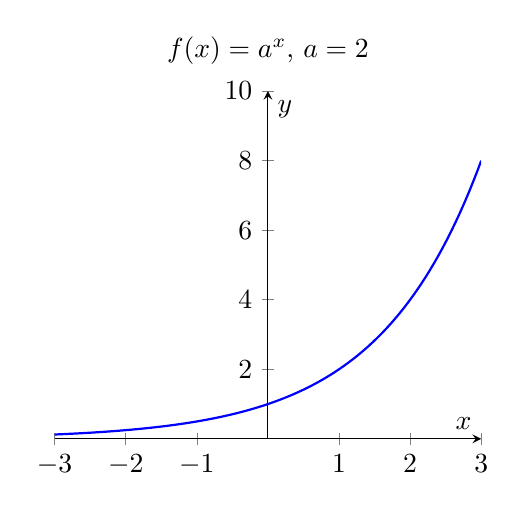
\begin{tikzpicture}
  \begin{axis}[
    title={$f(x) = a^x$, $a=2$},
    axis lines=middle,
    xlabel=$x$, ylabel=$y$,
    domain=-3:3,
    samples=100,
    width=7cm, height=6cm,
    ymin=0, ymax=10,
  ]
    \addplot[blue, thick] {2^x};
  \end{axis}
\end{tikzpicture}

}
\end{tabularx}


\begin{tabularx}{\textwidth}{X r} 
\vprasanje{Naj bo $0<a<1$. Narišite graf funkcije s predpisom $f(x)=a^x$.}{2 točki}
\odgovor{
\begin{itemize}
  \item Graf funkcije $f(x) = a^x$ za $0 < a < 1$ je eksponentna krivulja, ki:
  \begin{itemize}
    \item poteka skozi točko $(0,1)$,
    \item hitro pada za $x > 0$,
    \item se približuje osi $x$ za $x \to \infty$ (asimptota $y = 0$),
    \item je strogo padajoča.
  \end{itemize}
\end{itemize}

\centering
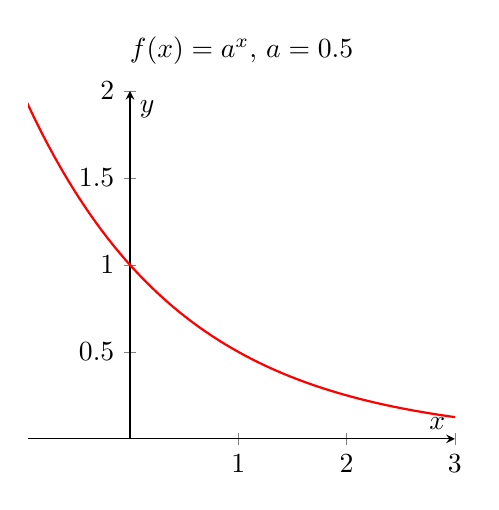
\begin{tikzpicture}
  \begin{axis}[
    title={$f(x) = a^x$, $a=0.5$},
    axis lines=middle,
    xlabel=$x$, ylabel=$y$,
    domain=-3:3,
    samples=100,
    width=7cm, height=6cm,
    ymin=0, ymax=2,
  ]
    \addplot[red, thick] {0.5^x};
  \end{axis}
\end{tikzpicture}

}
\end{tabularx}


\begin{tabularx}{\textwidth}{X r}
\vprasanje{Povejte štiri lastnosti eksponentne funkcije.}{2 točki}
\odgovor{
\begin{itemize}
  \item Definicijsko območje je $\mathbb{R}$.
  \item Zaloga vrednosti je $(0, \infty)$.
  \item Graf poteka skozi točko $(0,1)$.
  \item Je strogo monotona (narašča za $a > 1$, pada za $0 < a < 1$).
\end{itemize}
}
\end{tabularx}

\razmak{0.5em}


% ******** 64. Logaritemska funkcija ********
\crta

\naslov{Logaritemska funkcija}

\begin{tabularx}{\textwidth}{X r}
\vprasanje{Naj bo $a$ pozitivno realno število, $a \neq 1$. Definirajte logaritemsko funkcijo z osnovo $a$.}{1 točka}
\odgovor{
\begin{itemize}
  \item Logaritemska funkcija z osnovo $a$ je funkcija $f(x) = \log_a x$, kjer je $a > 0$ in $a \neq 1$.
  \item Določa potenco, na katero moramo potencirati število $a$, da dobimo $x$, torej: 
  
  \[
  \log_a b = c \iff a^c = b
  \]
  
\end{itemize}
}
\end{tabularx}

\begin{tabularx}{\textwidth}{X r}
\vprasanje{Naj bo $a>1$. Narišite graf logaritemske funkcije z osnovo $a$.}{2 točki}
\odgovor{
\begin{itemize}
  \item Graf funkcije $f(x) = \log_a x$ za $a > 1$:
  \begin{itemize}
    \item poteka skozi točko $(1,0)$,
    \item je strogo naraščajoč,
    \item se približuje osi $y$ (asimptota $x = 0$),
    \item definiran je za $x > 0$.
  \end{itemize}
\end{itemize}

\centering
\begin{tikzpicture}
  \begin{axis}[
    title={$f(x) = \log_2 x$},
    axis lines=middle,
    xlabel=$x$, ylabel=$y$,
    domain=0.01:5,
    samples=100,
    width=7cm, height=6cm,
    ymin=-3, ymax=3,
    restrict x to domain=0.01:5,
  ]
    \addplot[blue, thick] {ln(x)/ln(2)};
  \end{axis}
\end{tikzpicture}

}
\end{tabularx}

\begin{tabularx}{\textwidth}{X r}
\vprasanje{Naj bo $0<a<1$. Narišite graf logaritemske funkcije z osnovo $a$.}{2 točki}
\odgovor{
\begin{itemize}
  \item Graf funkcije $f(x) = \log_a x$ za $0 < a < 1$:
  \begin{itemize}
    \item poteka skozi točko $(1,0)$,
    \item je strogo padajoč,
    \item se približuje osi $y$ (asimptota $x = 0$),
    \item definiran je za $x > 0$.
  \end{itemize}
\end{itemize}

\centering
\begin{tikzpicture}
  \begin{axis}[
    title={$f(x) = \log_{\frac{1}{2}} x$},
    axis lines=middle,
    xlabel=$x$, ylabel=$y$,
    domain=0.01:5,
    samples=100,
    width=7cm, height=6cm,
    ymin=-3, ymax=3,
    restrict x to domain=0.01:5,
  ]
    \addplot[red, thick] {ln(x)/ln(0.5)};
  \end{axis}
\end{tikzpicture}
}
\end{tabularx}


\begin{tabularx}{\textwidth}{X r}
\vprasanje{Povejte dve lastnosti logaritemske funkcije.}{1 točka}
\odgovor{
\begin{itemize}
  \item Definicijsko območje je $(0, \infty)$.
  \item Zaloga vrednosti je $\mathbb{R}$.
\end{itemize}
}
\end{tabularx}

\razmak{0.5em}


% ******** 65. Računanje z logaritmi ********
\crta

\naslov{Računanje z logaritmi}

\begin{tabularx}{\textwidth}{X r}
\vprasanje{Povejte definicijo logaritma $\log _e x$.}{1 točka}
\odgovor{
\begin{itemize}
  \item Logaritem z osnovo $e$ (Eulerjevo število) je naravni logaritem: $\log_e x = \ln x$.
  \item To je potenca, na katero moramo potencirati število $e \approx 2{,}718$ (Eulerjevo število), da dobimo $x$.
\end{itemize}
}
\end{tabularx}

\begin{tabularx}{\textwidth}{X r}
\vprasanje{Povejte pravila za logaritem produkta, logaritem kvocienta in logaritem potence.}{3 točke}
\odgovor{
\begin{itemize}
  \item $\log_a(x \cdot y) = \log_a x + \log_a y$ \hfill (produkt)
  \item $\log_a\left(\frac{x}{y}\right) = \log_a x - \log_a y$ \hfill (kvocient)
  \item $\log_a(x^n) = n \cdot \log_a x$ \hfill (potenca)
\end{itemize}
}
\end{tabularx}

\begin{tabularx}{\textwidth}{X r}
\vprasanje{Koliko je $\log _0 1, \log _0 a, e^{i \pi x}$ in $\log 10^x$ ?}{2 točki}
\odgovor{
\begin{itemize}
  \item $\log_0 1$ ni definiran, ker osnova logaritma ne sme biti $0$.
  \item $\log_0 a$ prav tako ni definiran (enak razlog).
  \item $e^{i\pi x} = \cos(\pi x) + i \sin(\pi x)$ \hfill (Eulerjeva formula)
  \item $\log 10^x = x \cdot \log 10 = x$ \hfill (ker $\log$ pomeni $\log_{10}$)
\end{itemize}
}
\end{tabularx}

\razmak{0.5em}


% ******** 66. Polinomi ********
\crta

\naslov{Polinomi}

\begin{tabularx}{\textwidth}{X r}
\vprasanje{Definirajte polinom (polinomsko funkcijo). Kaj so stopnja, vodilni koeficient in prosti člen polinoma?}{2 točki}
\odgovor{
\begin{itemize}
  \item Polinom je funkcija oblike $f(x) = a_nx^n + a_{n-1}x^{n-1} + \dots + a_1x + a_0$, kjer so $a_i \in \mathbb{R}$, $n \in \mathbb{N}_0$.
  \item Stopnja polinoma je največji eksponent pri $x$ z neničelnim koeficientom ($n$).
  \item Vodilni koeficient je koeficient ob najvišji potenci ($a_n$).
  \item Prosti člen je člen brez spremenljivke ($a_0$).
\end{itemize}
}
\end{tabularx}

\begin{tabularx}{\textwidth}{X r}
\vprasanje{Kako množimo polinome? Kakšna je stopnja produkta dveh polinomov?}{2 točki}
\odgovor{
\begin{itemize}
  \item Vsak člen prvega polinoma pomnožimo z vsakim členom drugega polinoma.
  \item Nato poenostavimo: združimo podobne člene.
  \item Stopnja produkta je vsota stopenj obeh polinomov.
\end{itemize}
}
\end{tabularx}

\begin{tabularx}{\textwidth}{X r}
\vprasanje{Povejte osnovni izrek o deljenju polinomov.}{2 točki}
\odgovor{
\begin{itemize}
  \item Za polinoma $f(x)$ in $g(x) \ne 0$ obstajata enolično določena polinoma $q(x)$ in $r(x)$, da velja:
  \[
  f(x) = g(x) \cdot q(x) + r(x)
  \]
  \item pri čemer je $r(x)$ ničelni polinom ali pa ima \textbf{stopnjo manjšo od stopnje polinoma} $g(x)$.
\end{itemize}
}
\end{tabularx}

\razmak{0.5em}


% ******** 67. Ničle polinomov ********
\crta

\naslov{Ničle polinomov}

\begin{tabularx}{\textwidth}{X r}
\vprasanje{Največ koliko realnih ničel ima lahko polinom stopnje $n$ ?}{1 točka}
\odgovor{
\begin{itemize}
  \item Polinom stopnje $n$ ima lahko največ $n$ realnih ničel.
\end{itemize}
}
\end{tabularx}

\begin{tabularx}{\textwidth}{X r}
\vprasanje{Polinom $p$ stopnje $n$ naj ima $n$ paroma različnih ničel Kako lahko zapišemo predpis polinoma $p$, da bodo iz njega razvidne vse njegove ničle?}{1 točka}
\odgovor{
\begin{itemize}
  \item Polinom zapišemo kot: $p(x) = a(x - x_1)(x - x_2)\dots(x - x_n)$, kjer so $x_1, \dots, x_n$ njegove ničle.
\end{itemize}
}
\end{tabularx}

\begin{tabularx}{\textwidth}{X r}
\vprasanje{Koliko realnih ničel ima lahko polinom tretje stopnje? Navedite vse možnosti.}{2 točki}
\odgovor{
\begin{itemize}
  \item Polinom tretje stopnje ima lahko:
  \begin{itemize}
    \item eno realno ničlo (in dve kompleksni konjugirani),
    \item tri realne ničle (vse različne ali nekatere enake).
  \end{itemize}
\end{itemize}
}
\end{tabularx}

\begin{tabularx}{\textwidth}{X r}
\vprasanje{Povejte primer polinoma četrte stopnje z realnimi koeficienti, ki ima natanko dve različni realni ničli.}{2 točki}
\odgovor{
\begin{itemize}
  \item Primer: $f(x) = (x - 1)^2(x + 2)^2$
  \item Realni ničli sta $x = 1$ in $x = -2$.
\end{itemize}
}
\end{tabularx}

\razmak{0.5em}


% ******** 68. Racionalna funkcija ********
\crta

\naslov{Racionalna funkcija}

\begin{tabularx}{\textwidth}{X r}
\vprasanje{Kako poiščemo ničle in pole racionalne funkcije?}{2 točki}
\odgovor{
\begin{itemize}
  \item Racionalna funkcija je oblike $f(x) = \frac{p(x)}{q(x)}$, kjer sta $p(x)$ in $q(x)$ polinoma.
  \item \textbf{Ničle funkcije}: rešimo enačbo $p(x) = 0$ in hkrati preverimo, da $q(x) \neq 0$.
  \item \textbf{Poli funkcije}: poiščemo vrednosti $x$, za katere velja $q(x) = 0$, a $p(x) \neq 0$.
\end{itemize}
}
\end{tabularx}

\begin{tabularx}{\textwidth}{X r}
\vprasanje{Naj bo $x_0$ ničla racionalne funkcije $f$. Razložite obnašanje funkcije $f$ v dovolj majhni okolici ničle $x_0$. Navedite vse možnosti.}{2 točki}
\odgovor{
\begin{itemize}
  \item Če je $x_0$ ničla \textbf{sode} stopnje: funkcija ne spremeni predznaka pri prehodu skozi $x_0$ (graf se dotakne osi $x$).
  \item Če je $x_0$ ničla \textbf{lihe} stopnje: funkcija spremeni predznak (graf seka os $x$).
  \item V obeh primerih je $f(x_0) = 0$.
\end{itemize}
}
\end{tabularx}

\begin{tabularx}{\textwidth}{X r}
\vprasanje{Naj bo $x_0$ pol racionalne funkcije $f$. Razložite obnašanje funkcije $f$ v dovolj majhni okolici pola $x_0$. Navedite vse možnosti.}{2 točki}
\odgovor{
\begin{itemize}
  \item Če ima pol $x_0$ \textbf{lihe} stopnje: funkcija ima predznak različne strani odvisno od lim $x \to x_0^\pm$.
  \item Če ima pol $x_0$ \textbf{sode} stopnje: funkcija se z obeh strani približuje isti neskončnosti ($+\infty$ ali $-\infty$).
  \item V vsakem primeru je $f(x)$ v okolici $x_0$ neskončno velika (navzgor ali navzdol), funkcija tam ni definirana.
\end{itemize}
}
\end{tabularx}

\razmak{0.5em}


% ******** 69. Racionalna funkcija ********
\crta

\naslov{Racionalna funkcija}

\begin{tabularx}{\textwidth}{X r}
\vprasanje{Naj ima racionalna funkcija $f$ vse ničle in pole na intervalu $(a, b)$. Razložite obnašanje racionalne funkcije $f$ izven intervala $(a, b)$. Navedite vse možnosti.}{3 točke}
\odgovor{
\begin{itemize}
  \item Ker zunaj intervala $(a, b)$ ni ničel in polov, je funkcija tam zvezna in definirana.
  \item Možnosti za obnašanje funkcije:
  \begin{itemize}
    \item Lahko se približuje vodoravni asimptoti (če obstaja).
    \item Lahko se približuje poševni asimptoti (če obstaja).
    \item Lahko raste ali pada proti $\pm\infty$, če ni asimptote.
  \end{itemize}
  \item Funkcija izven $(a, b)$ nima prekinitev ali nedefiniranih točk.
\end{itemize}
}
\end{tabularx}

\begin{tabularx}{\textwidth}{X r}
\vprasanje{Kdaj ima graf racionalne funkcije vodoravno asimptoto? Kako izračunamo njeno enačbo?}{2 točki}
\odgovor{
\begin{itemize}
  \item Če sta $n$ in $m$ stopnji števca in imenovalca:
  \begin{itemize}
    \item Če $n < m$: $y = 0$ je vodoravna asimptota.
    \item Če $n = m$: $y = \frac{a_n}{b_m}$, kjer sta $a_n$, $b_m$ vodilna koeficienta.
    \item Če $n > m$: vodoravne asimptote ne obstajajo.
  \end{itemize}
\end{itemize}
}
\end{tabularx}

\begin{tabularx}{\textwidth}{X r}
\vprasanje{Povejte primer racionalne funkcije, katere graf ima asimptoto z enačbo $y=2$.}{1 točka}
\odgovor{
\begin{itemize}
  \item Primer: $f(x) = \frac{6x^2 + 1}{3x^2 - 4}$ 
  \item V tem primeru sta stopnji enaki ($n = m = 2$) in $\frac{6}{3} = 2$.
\end{itemize}
}
\end{tabularx}

\razmak{0.5em}


% ******** 70. Funkcija sinus ********
\crta

\naslov{Funkcija sinus}

\begin{tabularx}{\textwidth}{X r}
\vprasanje{Definirajte funkcijo sinus.}{1 točka}
\odgovor{
\begin{itemize}
  \item Funkcija sinus je definirana kot $f(x) = \sin(x)$, kjer je $x$ realno število, ki predstavlja kot v radianih.
  \item V pravokotnem trikotniku je sinus razmerje med dolžino nasprotne katete in dolžino hipotenuze.
  \item V enotskem krogu je $\sin(x)$ ordinata točke na krožnici, ki jo opiše kot $x$.
\end{itemize}
}
\end{tabularx}

\begin{tabularx}{\textwidth}{X r}
\vprasanje{Koliko je osnovna perioda funkcije sinus? Povejte vse ničle funkcije sinus.}{2 točki}
\odgovor{
\begin{itemize}
  \item Osnovna perioda funkcije sinus je $2\pi$.
  \item Vse ničle so točke $x = k\pi$, kjer je $k$ poljubno celo število ($k \in \mathbb{Z}$).
\end{itemize}
}
\end{tabularx}

\begin{tabularx}{\textwidth}{X r}
\vprasanje{V katerih točkah ima funkcija sinus maksimum in v katerih minimum?}{2 točki}
\odgovor{
\begin{itemize}
  \item Maksimumi so v točkah $x = \frac{\pi}{2} + 2k\pi$, kjer je vrednost $\sin x = 1$.
  \item Minimumi so v točkah $x = \frac{3\pi}{2} + 2k\pi$, kjer je vrednost $\sin x = -1$.
  \item $k$ je poljubno celo število ($k \in \mathbb{Z}$).
\end{itemize}
}
\end{tabularx}

\begin{tabularx}{\textwidth}{X r}
\vprasanje{Narišite graf funkcije sinus.}{1 točka}
\odgovor{
\begin{itemize}
  \item Graf funkcije sinus je gladka, periodična valovita krivulja, ki se ponavlja vsakih $2\pi$.
  \item Začne se v koordinatnem izhodišču $(0,0)$, se povzpne do maksimuma 1 pri $\pi/2$, nato spusti do ničle pri $\pi$, nadaljuje do minimuma $-1$ pri $3\pi/2$ in se vrne do ničle pri $2\pi$.
\end{itemize}

\centering
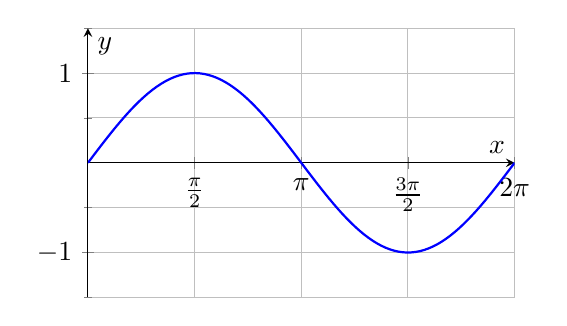
\begin{tikzpicture}
  \begin{axis}[
    axis lines=middle,
    xlabel=$x$, ylabel=$y$,
    domain=0:2*pi,
    samples=100,
    xtick={0,pi/2,pi,3*pi/2,2*pi},
    xticklabels={$0$, $\frac{\pi}{2}$, $\pi$, $\frac{3\pi}{2}$, $2\pi$},
    ymin=-1.5, ymax=1.5,
    width=7cm, height=5cm,
    grid=both,
    minor tick num=1,
  ]
    \addplot[blue, thick] {sin(deg(x))};
  \end{axis}
\end{tikzpicture}
}
\end{tabularx}


\razmak{0.5em}


% ******** 71. Funkcija kosinus ********
\crta

\naslov{Funkcija kosinus}

\begin{tabularx}{\textwidth}{X r}
\vprasanje{Definirajte funkcijo kosinus.}{1 točka}
\odgovor{
\begin{itemize}
  \item Funkcija kosinus je definirana kot $f(x) = \cos(x)$, kjer je $x$ realno število, ki predstavlja kot v radianih.
  \item V pravokotnem trikotniku je kosinus razmerje med dolžino pripadajoče katete in dolžino hipotenuze.
  \item V enotskem krogu je $\cos(x)$ abscisa točke na krožnici, ki jo opiše kot $x$.
\end{itemize}
}
\end{tabularx}

\begin{tabularx}{\textwidth}{X r}
\vprasanje{Koliko je osnovna perioda funkcije kosinus? Povejte vse ničle funkcije kosinus.}{2 točki}
\odgovor{
\begin{itemize}
  \item Osnovna perioda funkcije kosinus je $2\pi$.
  \item Vse ničle so točke $x = \frac{\pi}{2} + k\pi$, kjer je $k$ poljubno celo število.
\end{itemize}
}
\end{tabularx}

\begin{tabularx}{\textwidth}{X r}
\vprasanje{V katerih točkah ima funkcija kosinus maksimum in v katerih minimum?}{2 točki}
\odgovor{
\begin{itemize}
  \item Maksimumi so v točkah $x = 2k\pi$, kjer je vrednost $\cos x = 1$.
  \item Minimumi so v točkah $x = \pi + 2k\pi$, kjer je vrednost $\cos x = -1$.
  \item $k$ je poljubno celo število.
\end{itemize}
}
\end{tabularx}

\begin{tabularx}{\textwidth}{X r}
\vprasanje{Narišite graf funkcije kosinus.}{1 točka}
\odgovor{
\begin{itemize}
  \item Graf funkcije kosinus je gladka, periodična valovita krivulja s periodo $2\pi$.
  \item Začne se v točki $(0,1)$, pada do ničle pri $\frac{\pi}{2}$, doseže minimum $-1$ pri $\pi$, se vrne do ničle pri $\frac{3\pi}{2}$ in zaključuje cikel pri $2\pi$ na vrednosti 1.
\end{itemize}

\centering
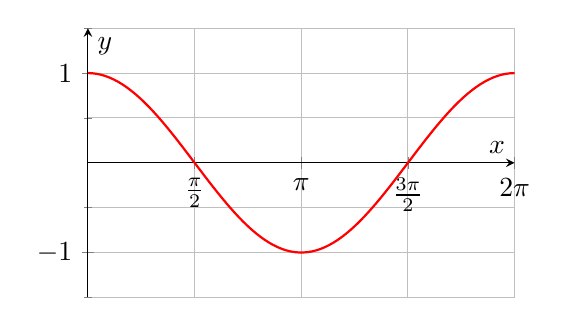
\begin{tikzpicture}
  \begin{axis}[
    axis lines=middle,
    xlabel=$x$, ylabel=$y$,
    domain=0:2*pi,
    samples=100,
    xtick={0,pi/2,pi,3*pi/2,2*pi},
    xticklabels={$0$, $\frac{\pi}{2}$, $\pi$, $\frac{3\pi}{2}$, $2\pi$},
    ymin=-1.5, ymax=1.5,
    width=7cm, height=5cm,
    grid=both,
    minor tick num=1,
  ]
    \addplot[red, thick] {cos(deg(x))};
  \end{axis}
\end{tikzpicture}
}
\end{tabularx}


\razmak{0.5em}


% ******** 72. Funkcija tangens ********
\crta

\naslov{Funkcija tangens}

\begin{tabularx}{\textwidth}{X r}
\vprasanje{Definirajte funkcijo tangens.}{1 točka}
\odgovor{
\begin{itemize}
  \item Funkcija tangens je definirana kot $f(x) = \tan(x) = \dfrac{\sin(x)}{\cos(x)}$.
  \item V pravokotnem trikotniku je tangens razmerje med nasprotno kateto in pripadajočo kateto.
\end{itemize}
}
\end{tabularx}

\begin{tabularx}{\textwidth}{X r}
\vprasanje{Povejte definicijsko območje funkcije tangens.}{1 točka}
\odgovor{
\begin{itemize}
  \item Tangens ni definiran tam, kjer je $\cos(x) = 0$.
  \item Definicijsko območje je množica vseh realnih števil razen $x = \frac{\pi}{2} + k\pi$, kjer je $k \in \mathbb{Z}$.
\end{itemize}
}
\end{tabularx}

\begin{tabularx}{\textwidth}{X r}
\vprasanje{Koliko je osnovna perioda funkcije tangens? Povejte vse ničle funkcije tangens.}{2 točki}
\odgovor{
\begin{itemize}
  \item Osnovna perioda funkcije tangens je $\pi$.
  \item Vse ničle so v točkah $x = k\pi$, kjer je $k \in \mathbb{Z}$.
\end{itemize}
}
\end{tabularx}

\begin{tabularx}{\textwidth}{X r}
\vprasanje{Narišite graf funkcije tangens.}{2 točki}
\odgovor{
\begin{itemize}
  \item Graf funkcije tangens je sestavljen iz ponavljajočih se ``vej`` z navpičnimi asimptotami v točkah $x = \frac{\pi}{2} + k\pi$.
  \item Vsaka veja se dviga iz $-\infty$ v $+\infty$ in prečka izhodišče (0,0).
  \item Graf nima maksimumov ali minimumov.
\end{itemize}

\centering
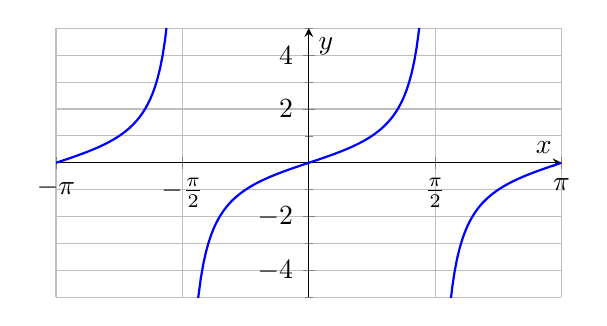
\begin{tikzpicture}
  \begin{axis}[
    axis lines=middle,
    xlabel=$x$, ylabel=$y$,
    domain=-pi:pi,
    samples=200,
    xtick={-pi, -pi/2, 0, pi/2, pi},
    xticklabels={$-\pi$, $-\frac{\pi}{2}$, $0$, $\frac{\pi}{2}$, $\pi$},
    ymin=-5, ymax=5,
    width=8cm, height=5cm,
    grid=both,
    minor tick num=1,
    restrict y to domain=-10:10,
    clip=true,
  ]
    \addplot[blue, thick] {tan(deg(x))};
  \end{axis}
\end{tikzpicture}
}
\end{tabularx}


\razmak{0.5em}


% ******** 73. Kotne funkcije ********
\crta

\naslov{Kotne funkcije}

\begin{tabularx}{\textwidth}{X r}
\vprasanje{Za vsako izmed kotnih funkcij sinus, kosinus in tangens povejte, ali je soda oziroma liha.}{2 točki}
\odgovor{
\begin{itemize}
  \item Sinus: liha funkcija.
  \item Kosinus: soda funkcija.
  \item Tangens: liha funkcija.
\end{itemize}
}
\end{tabularx}

\begin{tabularx}{\textwidth}{X r}
\vprasanje{Utemeljite odgovore iz prvega vprašanja.}{2 točki}
\odgovor{
\begin{itemize}
  \item $\sin(-x) = -\sin(x)$ \quad (definicija lihe funkcije)
  \item $\cos(-x) = \cos(x)$ \quad (definicija sode funkcije)
  \item $\tan(-x) = -\tan(x)$ \quad (definicija lihe funkcije, saj je tangens količnik lihe in sode funkcije: $\frac{\sin(-x)}{\cos(-x)} = \frac{-\sin x}{\cos x} = -\tan x$)
\end{itemize}
}
\end{tabularx}

\begin{tabularx}{\textwidth}{X r}
\vprasanje{Izrazite $\sin \left(200^{\circ}\right)$ in $\cos \left(115^{\circ}\right)$ z vrednostjo kotne funkcije ostrega kota.}{2 točki}
\odgovor{
\begin{itemize}
  \item $\sin(200^\circ) = -\sin(20^\circ)$, ker je $200^\circ = 180^\circ + 20^\circ$ in sinus je v tretjem kvadrantu negativen.
  \item $\cos(115^\circ) = -\cos(65^\circ)$, ker je $115^\circ = 180^\circ - 65^\circ$ in kosinus je v drugem kvadrantu negativen.
\end{itemize}
}
\end{tabularx}

\razmak{0.5em}


% ******** 74. Kotne funkcije v pravokotnem trikotniku ********
\crta

\naslov{Kotne funkcije v pravokotnem trikotniku}

\begin{tabularx}{\textwidth}{X r}
\vprasanje{Naj bo $\alpha$ ostri kot v danem pravokotnem trikotniku. Definirajte sinus, kosinus, tangens in kotangens kota $\alpha$.}{2 točki}
\odgovor{
\begin{itemize}
  \item $\sin \alpha = \dfrac{\text{nasprotna kateta}}{\text{hipotenuza} }$
  \item $\cos \alpha = \dfrac{\text{priležna kateta}}{\text{hipotenuza} }$
  \item $\tan \alpha = \dfrac{\text{nasprotna kateta}}{\text{priležna kateta}}$
  \item $\cot \alpha = \dfrac{\text{priležna kateta}}{\text{nasprotna kateta}}$
\end{itemize}
}
\end{tabularx}

\begin{tabularx}{\textwidth}{X r}
\vprasanje{Naj bo $\alpha$ točka v prostoru $\mathbb{R}^3$. Povejte osnovno zvezo med $\sin \alpha$ in $\cos \alpha$ ter jo dokažite.}{2 točki}
\odgovor{
\textbf{Zveza:} $\sin^2 \alpha + \cos^2 \alpha = 1$
\textbf{Dokaz:} Naj bo $\alpha$ ostri kot v pravokotnem trikotniku. Označimo dolžino nasprotne katete z $a$, sosednje s $b$, in hipotenuze s $c$. Tedaj:
\[
\sin \alpha = \frac{a}{c}, \quad \cos \alpha = \frac{b}{c}
\]
\[
\sin^2 \alpha + \cos^2 \alpha = \left( \frac{a}{c} \right)^2 + \left( \frac{b}{c} \right)^2 = \frac{a^2 + b^2}{c^2}
\]
Po Pitagorovem izreku je $a^2 + b^2 = c^2$, zato:
\[
\sin^2 \alpha + \cos^2 \alpha = \frac{c^2}{c^2} = 1
\]
}
\end{tabularx}

\begin{tabularx}{\textwidth}{X r}
\vprasanje{Povejte še štiri zveze med kotnimi funkcijami v pravokotnem trikotniku.}{2 točki}
\odgovor{
\begin{itemize}
  \item $\tan \alpha = \dfrac{\sin \alpha}{\cos \alpha}$
  \item $\cot \alpha = \dfrac{\cos \alpha}{\sin \alpha}$
  \item $\tan \alpha = \dfrac{1}{\cot \alpha}$
  \item $\sin^2 \alpha + \cos^2 \alpha = 1$
\end{itemize}
}
\end{tabularx}

\razmak{0.5em}


% ******** 75. Kotne funkcije ********
\crta

\naslov{Kotne funkcije}

\begin{tabularx}{\textwidth}{X r}
\vprasanje{Povejte adicijska izreka za funkciji sinus in kosinus.}{2 točki}
\odgovor{
\begin{itemize}
  \item $\sin(a + b) = \sin a \cos b + \cos a \sin b$
  \item $\cos(a + b) = \cos a \cos b - \sin a \sin b$
\end{itemize}
}
\end{tabularx}

\begin{tabularx}{\textwidth}{X r}
\vprasanje{Izrazite $\sin (2 x)$ in $\cos (2 x) \mathrm{s} \sin x$ in $\cos x$.}{2 točki}
\odgovor{
\begin{itemize}
  \item $\sin(2x) = 2 \sin x \cos x$
  \item $\cos(2x) = \cos^2 x - \sin^2 x$
\end{itemize}
}
\end{tabularx}

\begin{tabularx}{\textwidth}{X r}
\vprasanje{Rešite enačbo $\sin (2 x)=\sin x$.}{2 točki}
\odgovor{
\[
	\begin{array}{rcl}
	\sin(2x) &= \sin x \\
	2 \sin x \cos x &   = \sin x \\
	\sin x (2 \cos x - 1) &= 0 
	\end{array}
\]

Enačba je izpolnjena, če je:
\begin{itemize}
  \item $\sin x = 0 \quad \Rightarrow \quad x = k\pi, \; k \in \mathbb{Z}$
  \item $2 \cos x - 1 = 0 \quad \Rightarrow \quad \cos x = \frac{1}{2} \quad \Rightarrow \quad x = \pm \frac{\pi}{3} + 2k\pi, \; k \in \mathbb{Z}$
\end{itemize}
Skupna rešitev:
\[
x = k\pi \quad \text{ali} \quad x = \pm \frac{\pi}{3} + 2k\pi, \; k \in \mathbb{Z}
\]
}
\end{tabularx}

\razmak{0.5em}

% ******** 76. Kotne funkcije ********
\crta

\naslov{Kotne funkcije}

\begin{tabularx}{\textwidth}{X r}
\vprasanje{V isti koordinatni sistem narišite grafa funkcij sinus in kosinus.}{2 točki}
\odgovor{
\begin{itemize}
	\item Graf funkcije $\sin x$ je valovanje, ki se začne v točki $(0, 0)$, medtem ko se $\cos x$ začne v točki $(0, 1)$. Oba grafa imata osnovno periodo $2\pi$, amplitudo $1$, in potekata med $-1$ in $1$.
\end{itemize}

\centering
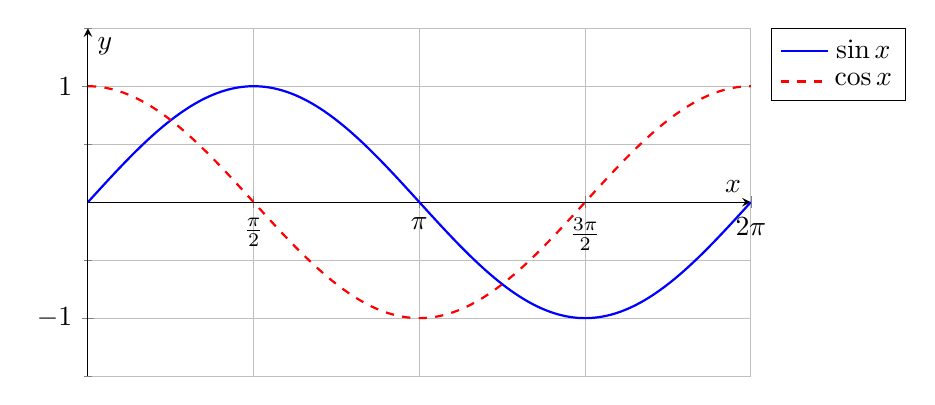
\begin{tikzpicture}
  \begin{axis}[
    axis lines=middle,
    xlabel=$x$, ylabel=$y$,
    domain=0:2*pi,
    samples=200,
    xtick={0, pi/2, pi, 3*pi/2, 2*pi},
    xticklabels={$0$, $\frac{\pi}{2}$, $\pi$, $\frac{3\pi}{2}$, $2\pi$},
    ymin=-1.5, ymax=1.5,
    width=10cm, height=6cm,
    legend pos=outer north east,
    grid=both,
    minor tick num=1,
  ]
    \addplot[blue, thick] {sin(deg(x))};
    \addplot[red, thick, dashed] {cos(deg(x))};
    \legend{$\sin x$, $\cos x$}
  \end{axis}
\end{tikzpicture}
}
\end{tabularx}


\begin{tabularx}{\textwidth}{X r}
\vprasanje{Povejte vsaj dve lastnosti funkcij, ki sta skupni funkcijama sinus in kosinus.}{1 točka}
\odgovor{
\begin{itemize}
  \item Obe funkciji sta periodični z osnovno periodo $2\pi$.
  \item Obe funkciji sta omejeni z vrednostmi med $-1$ in $1$.
\end{itemize}
}
\end{tabularx}

\begin{tabularx}{\textwidth}{X r}
\vprasanje{Povejte vsaj dve lastnosti funkcij, v katerih se funkciji sinus in kosinus razlikujeta.}{1 točka}
\odgovor{
\begin{itemize}
  \item Funkcija $\sin x$ je liha, $\cos x$ pa je soda.
  \item $\sin x$ ima ničlo pri $x = 0$, $\cos x$ pa ima tam maksimum.
\end{itemize}
}
\end{tabularx}

\begin{tabularx}{\textwidth}{X r}
\vprasanje{Izračunajte vsa presečišča grafov funkcij sinus in kosinus.}{2 točki}
\odgovor{
\[
	\begin{array}{rcl}
	\sin x &= \cos x \\
	\tan x &= 1 \\
	x &= \frac{\pi}{4} + k\pi,\quad k \in \mathbb{Z}
	\end{array}
\]
Presečišča: $x = \frac{\pi}{4} + k\pi$, $k \in \mathbb{Z}$, torej točke:
\[
\left(\frac{\pi}{4} + k\pi, \; \sin\left(\frac{\pi}{4} + k\pi\right)\right)
\]
}
\end{tabularx}
\razmak{0.5em}


% ******** 77. Krožnica ********
\crta

\naslov{Krožnica}

\begin{tabularx}{\textwidth}{X r}
\vprasanje{Povejte geometrijsko definicijo krožnice.}{1 točka}
\odgovor{
\begin{itemize}
  \item Krožnica je množica vseh točk v ravnini, ki so enako oddaljene od dane točke, imenovane središče krožnice ($S$).
\end{itemize}
}
\end{tabularx}

\begin{tabularx}{\textwidth}{X r}
\vprasanje{Povejte in izpeljite enačbo krožnice s polmerom $r$ in s središčem v koordinatnem izhodišču.}{2 točki}
\odgovor{
\begin{itemize}
  \item Naj bo $S(0,0)$ središče krožnice in $T(x,y)$ poljubna točka na krožnici.
  \item Razdalja med $S$ in $T$ mora biti enaka $r$: $\sqrt{(x - 0)^2 + (y - 0)^2} = r$.
  \item Kvadriramo: $x^2 + y^2 = r^2$.
  \item To je enačba krožnice s središčem v izhodišču in polmerom $r$.
\end{itemize}
}
\end{tabularx}

\begin{tabularx}{\textwidth}{X r}
\vprasanje{Povejte enačbo krožnice s polmerom $r$ in s središčem v točki $S(p, q)$.}{1 točka}
\odgovor{
\begin{itemize}
  \item Enačba krožnice s središčem $S(p, q)$ in polmerom $r$ je: $(x - p)^2 + (y - q)^2 = r^2$.
\end{itemize}
}
\end{tabularx}

\begin{tabularx}{\textwidth}{X r}
\vprasanje{Izpeljite zvezo med realnima številoma $a$ in $b$, da bo enačba $x^2+y^2+2 a x+2 b y+4=0$ predstavljala krožnico.}{2 točka}
\odgovor{
\begin{itemize}
  \item Preoblikujemo enačbo z dopolnjevanjem kvadratov:
  \item $x^2 + 2a x + y^2 + 2b y + 4 = 0$
  \item $(x + a)^2 - a^2 + (y + b)^2 - b^2 + 4 = 0$
  \item $(x + a)^2 + (y + b)^2 = a^2 + b^2 - 4$
  \item To je enačba krožnice, če je desna stran pozitivna: $a^2 + b^2 - 4 > 0$
  \item Torej mora veljati: $a^2 + b^2 > 4$
\end{itemize}
}
\end{tabularx}

\razmak{0.5em}


% ******** 78. Elipsa ********
\crta

\naslov{Elipsa}

\begin{tabularx}{\textwidth}{X r}
\vprasanje{Povejte geometrijsko definicijo elipse.}{2 točki}
\odgovor{
\begin{itemize}
  \item Elipsa je množica vseh točk v ravnini, za katere je vsota razdalj do dveh danih točk (gorišč) stalna.
  \item Gorišči elipse imenujemo točki $F_1$ in $F_2$, stalna vsota razdalj pa je enaka dolžini velike osi.
\end{itemize}
}
\end{tabularx}

\begin{tabularx}{\textwidth}{X r}
\vprasanje{Povejte enačbo elipse s središčem v koordinatnem izhodišču in enačbo elipse s središčem v točki $S(p, q)$. V obeh primerih naj bosta osi elipse vzporedni koordinatnima osema.}{2 točki}
\odgovor{
\begin{itemize}
  \item Središče v izhodišču $(0,0)$:
  \[
  \frac{x^2}{a^2} + \frac{y^2}{b^2} = 1
  \]
  kjer je $a$ dolžina velike osi, $b$ pa dolžina male osi.
  \item Središče v točki $S(p, q)$:
  \[
  \frac{(x - p)^2}{a^2} + \frac{(y - q)^2}{b^2} = 1
  \]
\end{itemize}
}
\end{tabularx}

\begin{tabularx}{\textwidth}{X r}
\vprasanje{Povejte primer enačbe elipse s središčem v koordinatnem izhodišču in jo narišite. Izračunajte tudi njeni gorišči.}{2 točki}
\odgovor{
\begin{itemize}
  \item Primer enačbe: $\displaystyle \frac{x^2}{9} + \frac{y^2}{4} = 1$
  \item To je elipsa s veliko osjo $a = 3$ in malo osjo $b = 2$.
  \item Razdalja od središča do gorišč je $c = \sqrt{a^2 - b^2} = \sqrt{9 - 4} = \sqrt{5}$
  \item Gorišči sta: $F_1 = (-\sqrt{5}, 0)$ in $F_2 = (\sqrt{5}, 0)$
\end{itemize}

\centering
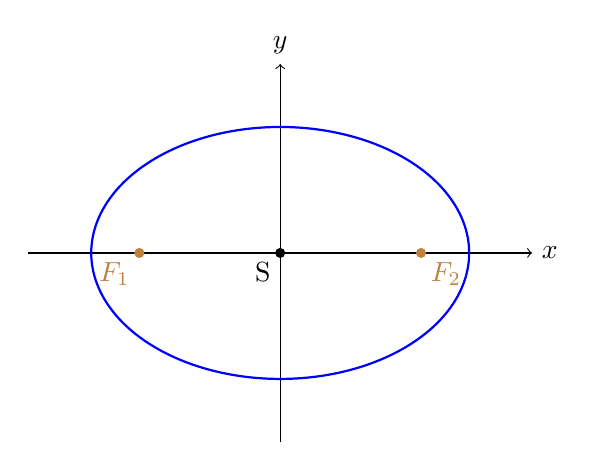
\begin{tikzpicture}[scale=0.8]
  \draw[->] (-4,0) -- (4,0) node[right] {$x$};
  \draw[->] (0,-3) -- (0,3) node[above] {$y$};
  
  \draw[thick, blue, domain=0:360, samples=100, smooth, variable=\t]
    plot ({3*cos(\t)}, {2*sin(\t)});

  \filldraw[brown] ({sqrt(5)}, 0) circle (2pt) node[below right] {$F_2$};
  \filldraw[brown] ({-sqrt(5)}, 0) circle (2pt) node[below left] {$F_1$};

  \filldraw (0,0) circle (2pt) node[below left] {S};
\end{tikzpicture}
}
\end{tabularx}

\razmak{0.5em}


% ******** 79. Hiperbola ********
\crta

\naslov{Hiperbola}

\begin{tabularx}{\textwidth}{X r}
\vprasanje{Povejte geometrijsko definicijo hiperbole.}{2 točki}
\odgovor{
\begin{itemize}
  \item Hiperbola je množica vseh točk v ravnini, za katere je absolutna vrednost razlike razdalj do dveh danih točk (gorišč) stalna.
  \item Gorišči hiperbole imenujemo točki $F_1$ in $F_2$, ta stalna razlika pa je enaka dolžini velike osi.
\end{itemize}
}
\end{tabularx}

\begin{tabularx}{\textwidth}{X r}
\vprasanje{Povejte enačbo hiperbole s središčem v koordinatnem izhodišču, katere osi ležita na koordinatnih oseh. Kako izračunamo enačbi njenih asimptot?}{2 točki}
\odgovor{
\begin{itemize}
  \item Enačba hiperbole z vodoravno osjo: $\displaystyle \frac{x^2}{a^2} - \frac{y^2}{b^2} = 1$
  \item Enačba hiperbole z navpično osjo: $\displaystyle \frac{y^2}{b^2} - \frac{x^2}{a^2} = 1$
  \item Enačbi asimptot hiperbole z vodoravno osjo:
  \[
  y = \pm \frac{b}{a}x
  \]
  \item Enačbi asimptot hiperbole z navpično osjo:
  \[
  y = \pm \frac{a}{b}x
  \]
\end{itemize}
}
\end{tabularx}

\begin{tabularx}{\textwidth}{X r}
\vprasanje{Povejte primer enačbe hiperbole s središčem v koordinatnem izhodišču in jo narišite. Izračunajte tudí njeni gorišči.}{2 točki}
\odgovor{
\begin{itemize}
  \item Primer enačbe: $\displaystyle \frac{x^2}{9} - \frac{y^2}{4} = 1$
  \item To je hiperbola z vodoravno osjo, kjer je $a = 3$ in $b = 2$
  \item Razdalja od središča do gorišč: $c = \sqrt{a^2 + b^2} = \sqrt{9 + 4} = \sqrt{13}$
  \item Gorišči sta: $F_1 = (-\sqrt{13}, 0)$ in $F_2 = (\sqrt{13}, 0)$
\end{itemize}

\centering
\begin{tikzpicture}
  \begin{axis}[
    axis lines=middle,
    xlabel=$x$, ylabel=$y$,
    xmin=-7, xmax=7,
    ymin=-5, ymax=5,
    samples=100,
    width=10cm, height=7cm,
    clip=false,
  ]

    \addplot[blue, thick, domain=-7:-3] {sqrt((x^2/9 - 1)*4)};
    \addplot[blue, thick, domain=-7:-3] {-sqrt((x^2/9 - 1)*4)};

    \addplot[blue, thick, domain=3:7] {sqrt((x^2/9 - 1)*4)};
    \addplot[blue, thick, domain=3:7] {-sqrt((x^2/9 - 1)*4)};

    \addplot[only marks, red] coordinates {({sqrt(13)}, 0) (-{sqrt(13)}, 0)};
  \end{axis}
\end{tikzpicture}
}
\end{tabularx}




\razmak{0.5em}

% ******** 80. Parabola ********
\crta

\naslov{Parabola}

\begin{tabularx}{\textwidth}{X r}
\vprasanje{Povejte geometrijsko definicijo parabole.}{2 točki}
\odgovor{
\begin{itemize}
  \item Parabola je množica vseh točk v ravnini, ki so enako oddaljene od dane točke (gorišča) in dane premice (vodnice).
\end{itemize}
}
\end{tabularx}

\begin{tabularx}{\textwidth}{X r}
\vprasanje{Povejte enačbo parabole s temenom v koordinatnem izhodišču in z goriščem na abscisni osi. Kako izračunamo gorišče in enačbo premice vodnice te parabole?}{3 točke}
\odgovor{
\begin{itemize}
  \item Enačba parabole z osjo simetrije vzporedno z $x$-osjo: $y^2 = 4px$
  \item Gorišče ima koordinati: $F = (p, 0)$
  \item Premica vodnica ima enačbo: $x = -p$
  \item Parameter $p$ določa razdaljo od temena do gorišča
\end{itemize}
}
\end{tabularx}

\begin{tabularx}{\textwidth}{X r}
\vprasanje{Povejte primer enačbe parabole s temenom v koordinatnem izhodišču in z goriščem na ordinatni osi.}{1 točka}
\odgovor{
\begin{itemize}
  \item Primer: $x^2 = 8y$
  \item To je parabola z osjo simetrije vzporedno z $y$-osjo in $p = 2$
  \item Gorišče ima koordinati: $F = (0, 2)$
\end{itemize}
}
\end{tabularx}

\razmak{0.5em}


% ******** 81. Zaporedja ********
\crta

\naslov{Zaporedja}

\begin{tabularx}{\textwidth}{X r}
\vprasanje{Definirajte zaporedje. Kaj je graf zaporedja?}{2 točki}
\odgovor{
\begin{itemize}
  \item Zaporedje je funkcija, ki vsakemu naravnemu številu $n$ ``priredi`` realno število $a_n$, tj. $a_1, a_2, a_3, \ldots$
  \item Graf zaporedja je množica točk v ravnini s koordinatami $(n, a_n)$, kjer je $n \in \mathbb{N}$
\end{itemize}
}
\end{tabularx}

\begin{tabularx}{\textwidth}{X r}
\vprasanje{Kdaj je zaporedje naraščajoče?}{1 točka}
\odgovor{
\begin{itemize}
  \item Zaporedje je naraščajoče, če za vsak $n \in \mathbb{N}$ velja $a_{n+1} > a_n$
\end{itemize}
}
\end{tabularx}

\begin{tabularx}{\textwidth}{X r}
\vprasanje{Predstavite primer padajočega zaporedja.}{1 točka}
\odgovor{
\begin{itemize}
  \item Primer: $a_n = \frac{1}{n}$
  \item Velja $a_{n+1} < a_n$ za vsak $n \in \mathbb{N}$
\end{itemize}
}
\end{tabularx}

\begin{tabularx}{\textwidth}{X r}
\vprasanje{Kdaj je zaporedje omejeno?}{1 točka}
\odgovor{
\begin{itemize}
  \item Zaporedje je omejeno, če obstajata realni števili $m$ in $M$, da za vse $n \in \mathbb{N}$ velja $m \leq a_n \leq M$
\end{itemize}
}
\end{tabularx}

\begin{tabularx}{\textwidth}{X r}
\vprasanje{Predstavite primer zaporedja, ki je navzgor omejeno, navzdol pa neomejeno.}{1 točka}
\odgovor{
\begin{itemize}
  \item Primer: $a_n = -n$
  \item Za vse $n$ velja $a_n \leq -1$, torej je zaporedje navzgor omejeno (npr. z $M = -1$), navzdol pa ni omejeno
\end{itemize}
}
\end{tabularx}
\razmak{0.5em}


% ******** 82. Aritmetično zaporedje ********
\crta

\naslov{Aritmetično zaporedje}

\begin{tabularx}{\textwidth}{X r}
\vprasanje{Definirajte aritmetično zaporedje in povejte njegov splošni člen.}{2 točki}
\odgovor{
\begin{itemize}
  \item Aritmetično zaporedje je zaporedje, kjer je razlika med zaporednima členoma vedno enaka, torej $a_{n+1} = a_n + d$
  \item Splošni člen aritmetičnega zaporedja je: $a_n = a_1 + (n - 1) d$
\end{itemize}
}
\end{tabularx}

\begin{tabularx}{\textwidth}{X r}
\vprasanje{Predstavite primer padajočega aritmetičnega zaporedja.}{1 točka}
\odgovor{
\begin{itemize}
  \item Primer: $a_n = 10 - 2(n - 1)$, torej zaporedje $10, 8, 6, 4, \ldots$
  \item Diferenca je negativna ($d = -2$), zato zaporedje pada
\end{itemize}
}
\end{tabularx}

\begin{tabularx}{\textwidth}{X r}
\vprasanje{Kako izračunamo vsoto prvih n členov aritmetičnega zaporedja, če poznamo prvi člen in diferenco?}{1 točka}
\odgovor{
\begin{itemize}
  \item Vsoto izračunamo po formuli: $S_n = \dfrac{n}{2} \left[2 a_1 + (n - 1) d \right]$
\end{itemize}
}
\end{tabularx}

\begin{tabularx}{\textwidth}{X r}
\vprasanje{Pokažite, da za poljubne tri zaporedne člene $a, b$ in $c$ aritmetičnega zaporedja velja, da je srednji člen $b$ enak aritmetični sredini sosednjih členov $a$ in $c$.}{2 točki}
\odgovor{
\begin{itemize}
  \item Naj bodo $a$, $b$, $c$ trije zaporedni členi aritmetičnega zaporedja, in $d$ diferenca. Torej velja:
  \item $b = a + d$, \quad $c = a + 2d$
  \item Potem je $\dfrac{a + c}{2} = \dfrac{a + (a + 2d)}{2} = \dfrac{2a + 2d}{2} = a + d = b$
  \item Torej velja: $b = \dfrac{a + c}{2}$
\end{itemize}
}
\end{tabularx}

\razmak{0.5em}


% ******** 83. Geometrijsko zaporedje ********
\crta

\naslov{Geometrijsko zaporedje}

\begin{tabularx}{\textwidth}{X r}
\vprasanje{Definirajte geometrijsko zaporedje in povejte njegov splošni člen.}{1 točka}
\odgovor{
\begin{itemize}
  \item Geometrijsko zaporedje je zaporedje, kjer je razmerje med zaporednima členoma vedno enako, torej $a_{n+1} = a_n \cdot q$
  \item Splošni člen geometrijskega zaporedja je: $a_n = a_1 \cdot q^{n - 1}$
\end{itemize}
}
\end{tabularx}

\begin{tabularx}{\textwidth}{X r}
\vprasanje{Predstavite primer padajočega geometrijskega zaporedja.}{1 točka}
\odgovor{
\begin{itemize}
  \item Primer: $a_n = 16 \cdot \left(\dfrac{1}{2}\right)^{n - 1}$, torej zaporedje $16, 8, 4, 2, \ldots$
  \item Količnik je $q = \dfrac{1}{2}$, zato zaporedje pada
\end{itemize}
}
\end{tabularx}

\begin{tabularx}{\textwidth}{X r}
\vprasanje{Kako izračunamo vsoto prvih n členov geometrijskega zaporedja, če poznamo prvi člen in količnik? Kako izračunamo to vsoto, če je količnik enak 1?}{2 točka}
\odgovor{
\begin{itemize}
  \item Če $q \neq 1$: $S_n = a_1 \cdot \dfrac{1 - q^n}{1 - q}$
  \item Če $q = 1$: $S_n = n \cdot a_1$
\end{itemize}
}
\end{tabularx}

\begin{tabularx}{\textwidth}{X r}
\vprasanje{Pokažite, da za poljubne tri zaporedne člene $a, b$ in $c$ geometrijskega zaporedja s pozitivnimi členi velja, da je srednji člen $b$ enak geometrijski sredini sosednjih členov $a$ in $c$.}{2 točka}
\odgovor{
\begin{itemize}
  \item Naj bo $b = a \cdot q$, \quad $c = a \cdot q^2$,\quad in $q$ količnik te vrste
  \item Potem je $\sqrt{a \cdot c} = \sqrt{a \cdot a q^2} = \sqrt{a^2 q^2} = a q = b$
  \item Torej velja: $b = \sqrt{a \cdot c}$
\end{itemize}
}
\end{tabularx}

\razmak{0.5em}


% ******** 84. Geometrijska vrsta ********
\crta

\naslov{Geometrijska vrsta}

\begin{tabularx}{\textwidth}{X r}
\vprasanje{Definiraj geometrijsko vrsto. Kako ugotovimo, ali je geometrijska vrsta konvergentna?}{2 točki}
\odgovor{
\begin{itemize}
  \item Geometrijska vrsta je vsota členov geometrijskega zaporedja: $a_1 + a_1 q + a_1 q^2 + \cdots$
  \item Vrsta je konvergentna, če je absolutna vrednost količnika $|q| < 1$
\end{itemize}
}
\end{tabularx}

\begin{tabularx}{\textwidth}{X r}
\vprasanje{Predstavite primer konvergentne in primer divergentne geometrijske vrste.}{2 točki}
\odgovor{
\begin{itemize}
  \item Konvergentna: $1 + \frac{1}{2} + \frac{1}{4} + \frac{1}{8} + \cdots$ \quad ($q = \frac{1}{2}$)
  \item Divergentna: $1 + 2 + 4 + 8 + \cdots$ \quad ($q = 2$)
\end{itemize}
}
\end{tabularx}

\begin{tabularx}{\textwidth}{X r}
\vprasanje{Kako izračunamo vsoto konvergentne geometrijske vrste, če poznamo prvi člen in količnik?}{1 točka}
\odgovor{
\begin{itemize}
  \item Če $|q| < 1$, potem je vsota: $S = \dfrac{a_1}{1 - q}$
\end{itemize}
}
\end{tabularx}

\begin{tabularx}{\textwidth}{X r}
\vprasanje{Izračunajte $1+\frac{1}{2}+\frac{1}{4}+\cdots$}{1 točka}
\odgovor{
\begin{itemize}
  \item Gre za konvergentno geometrijsko vrsto s $a_1 = 1$, $q = \frac{1}{2}$
  \item Vsota je: $S = \dfrac{1}{1 - \frac{1}{2}} = \dfrac{1}{\frac{1}{2}} = 2$
\end{itemize}
}
\end{tabularx}

\razmak{0.5em}


% ******** 85. Obrestni račun ********
\crta

\naslov{Obrestni račun}

\begin{tabularx}{\textwidth}{X r}
\vprasanje{Opišite osnovne pojme obrestno obrestnega računa: glavnica, obresti, obrestovalni faktor, kapitalizacijsko obdobje.}{4 točke}
\odgovor{
\begin{itemize}
  \item \textbf{Glavnica} ($G_0$): začetni vložek oziroma znesek denarja, ki ga vložimo na račun.
  \item \textbf{Obresti}: znesek, ki ga banka pripiše na glavnico kot nagrado za uporabo denarja.
  \item \textbf{Obrestovalni faktor} ($q$): faktor rasti kapitala v enem kapitalizacijskem obdobju, izražen kot $q = 1 + \frac{p}{100}$, kjer je $p$ letna obrestna mera v odstotkih.
  \item \textbf{Kapitalizacijsko obdobje}: časovni interval, po katerem se obresti pripišejo glavnici in se obrestujejo v naslednjih obdobjih (pri letnem pripisu je to eno leto).
\end{itemize}
}
\end{tabularx}

\begin{tabularx}{\textwidth}{X r}
\vprasanje{Kolikšen je privarčevani znesek po $n$ letih, če v banko vložimo glavnico $G_0$ po letni obrestni meri $p \%$? Banka uporablja obrestno obrestovanje z letnim pripisom obresti.}{2 točki}
\odgovor{
\begin{itemize}
  \item Privarčevani znesek po $n$ letih je: 
  \[
  G_n = G_0 \left(1 + \frac{p}{100}\right)^n = G_0 \cdot q^n,
  \]
  kjer je $q = 1 + \frac{p}{100}$ obrestovalni faktor.
\end{itemize}
}
\end{tabularx}

\razmak{0.5em}


% ******** 2. Odvod ********
\crta

\naslov{Odvod}

\begin{tabularx}{\textwidth}{X r}
\vprasanje{Definirajte odvod funkcije v dani točki in opišite njegov geometrijski pomen.}{2 točka}
\odgovor{
\begin{itemize}
  \item  Odvod predstavlja spremembo funkcije pri spremembi njenega argumenta. Opisuje najboljšo linearno aproksimacijo funkcije v bližini vrednosti funkcije z nekim argumentom.
  \item Odvod funkcije $f$ v točki $x_0$ je diferenčni količnik:
  \[
  f'(a) = \lim_{h \to 0} \frac{f(a + h) - f(a)}{h},
  \]
  če ta limit obstaja.
  \item Geometrijski pomen: odvod v točki $x_0$ predstavlja naklon tangente na graf funkcije $f$ v tej točki.
\end{itemize}
}
\end{tabularx}

\begin{tabularx}{\textwidth}{X r}
\vprasanje{Naj bo funkcija $f$ odvedljiva v točki $x_0$. Kako izračunamo enačbo tangente na graf funkcije $f$ v točki $x_0$ ?}{2 točki}
\odgovor{
\begin{itemize}
  \item Enačba tangente je:
  \[
  y = f(x_0) + f'(x_0)(x - x_0).
  \]
\end{itemize}
}
\end{tabularx}

\begin{tabularx}{\textwidth}{X r}
\vprasanje{Naj bo funkcija $f$ odvedljiva v točki $x_0$ in naj bo $f^{\prime}\left(x_0\right) \neq 0$. Kako izračunamo enačbo normale na graf funkcije $f$ v točki $x_0$ ?}{2 točki}
\odgovor{
\begin{itemize}
  \item Normalna je pravokotna na tangento, zato je njen naklon $m_n = -\frac{1}{f'(x_0)}$.
  \item Enačba normale je:
  \[
  y = f(x_0) - \frac{1}{f'(x_0)} (x - x_0).
  \]
\end{itemize}
}
\end{tabularx}

\razmak{0.5em}


% ******** 87. Lokalni ekstremi ********
\crta

\naslov{Lokalni ekstremi}

\begin{tabularx}{\textwidth}{X r}
\vprasanje{Definirajte lokalni maksimum in lokalni minimum funkcije.}{2 točki}
\odgovor{
\begin{itemize}
  \item Lokalni maksimum funkcije $f$ v točki $x_0$ je tak, da obstaja okolica $I$ točke $x_0$, kjer za vsak $x \in I$ velja:
  \[
  f(x) \leq f(x_0).
  \]
  \item Lokalni minimum funkcije $f$ v točki $x_0$ je tak, da obstaja okolica $I$ točke $x_0$, kjer za vsak $x \in I$ velja:
  \[
  f(x) \geq f(x_0).
  \]
\end{itemize}
}
\end{tabularx}

\begin{tabularx}{\textwidth}{X r}
\vprasanje{Naj bo $f: \mathbb{R} \rightarrow \mathbb{R}$ odvedljiva funkcija in $x_0$ njena stacionarna točka. Kako s pomočjo odvoda ugotovimo, ali ima funkcija v točki $x_0$ lokalni ekstrem?}{2 točki}
\odgovor{
\begin{itemize}
  \item $x_0$ je stacionarna točka, če je $f'(x_0) = 0$.
  \item Če je drugi odvod $f''(x_0) > 0$, ima funkcija v $x_0$ lokalni minimum.
  \item Če je drugi odvod $f''(x_0) < 0$, ima funkcija v $x_0$ lokalni maksimum.
  \item Če je $f''(x_0) = 0$, test je nezanesljiv in uporabimo test spremembe znaka odvoda, kjer:
  \begin{itemize}
  	\item Analiziramo spremembo znaka odvoda $f'(x_0)$ okoli točke $x_0$.
	\item Če $f'(x_0)$ prehaja iz $+$ v $-$, je lokalni maksimum.
	\item Če $f'(x_0)$ prehaja iz $-$ v $+$ znak, je lokalni minimum.
	\item Če se znak ne spremeni, ni lokalnega ekstrema.
  \end{itemize}
\end{itemize}
}
\end{tabularx}

\begin{tabularx}{\textwidth}{X r}
\vprasanje{Povejte primer funkcije, ki ima lokalni maksimum $M=3$ v točki $x_0=2$.}{1 točka}
\odgovor{
\[
f(x) = - (x-2)^2 + 3.
\]
}
\end{tabularx}

\begin{tabularx}{\textwidth}{X r}
\vprasanje{Povejte primer funkcije, ki nima lokalnih ekstremov.}{1 točka}
\odgovor{
\[
f(x) = x^3.
\]
Funkcija nima lokalnih maksimumov ali minimumov.
}
\end{tabularx}

\razmak{0.5em}


% ******** 88. Odvod ********
\crta

\naslov{Odvod}

\begin{tabularx}{\textwidth}{X r}
\vprasanje{
Naj bodo $a, b, c, k$ in $r$ poljubna realna števila. Izračunajte odvode funkcij:
\begin{itemize}[leftmargin=*, label={}]
  \item $f(x) = x^r$ \hfill (1 točka)
  \item $g(x) = a x^2 + b x + c$ \hfill (1 točka)
  \item $h(x) = \sin(a x) + b \cos x$ \hfill (1 točka)
  \item $t(x) = \tan x$ \hfill (1 točka)
  \item $s(x) = \mathrm{e}^{i x}$ \hfill (1 točka)
  \item $a(x) = \ln(\pi x + \pi^2)$ \hfill (1 točka)
\end{itemize}
\vspace{0.5em}
}{6 točk}
\odgovor{
\begin{itemize}[leftmargin=*, label={}]
  \item \( f(x) = x^r \implies f'(x) = r x^{r-1} \)
  \item \( g(x) = a x^2 + b x + c \implies g'(x) = 2 a x + b \)
  \item \( h(x) = \sin(a x) + b \cos x \implies h'(x) = a \cos(a x) - b \sin x \)
  \item \( t(x) = \tan x \implies t'(x) = \frac{1}{\cos^2 x} = \sec^2 x \)
  \item \( s(x) = \mathrm{e}^{i x} \implies s'(x) = i \mathrm{e}^{i x} \)
  \item \( a(x) = \ln(\pi x + \pi^2) \implies a'(x) = \frac{\pi}{\pi x + \pi^2} = \frac{1}{x + \pi} \)
\end{itemize}
}
\end{tabularx}

\razmak{0.5em}

% ******** 89. Odvod ********
\crta

\naslov{Odvod}

\begin{tabularx}{\textwidth}{X r}
\vprasanje{Naj graf odvedljive funkcije $f$ seka abcisno os v točki $T(x_0, 0)$. Povejte definicijo kota $\alpha$ med grafom funkcije $f$ in abcisno osjo v točki $T$. Kako izračunamo kot $\alpha$, če poznamo $f^{\prime}(x_0)$?}{2 točki}
\odgovor{
\begin{itemize}
  \item Kot $\alpha$ je kot med tangento na graf funkcije $f$ v točki $T$ in abcisno osjo (osjo $x$).
  \item Če je $f'(x_0)$ odvod v točki $x_0$, potem velja:
  \[
  \tan(\alpha) = f'(x_0) \implies \alpha = \arctan \bigl(f'(x_0)\bigr).
  \]
\end{itemize}
}
\end{tabularx}

\begin{tabularx}{\textwidth}{X r}
\vprasanje{Naj se grafa odvedljivih funkcij $f$ in $g$ sekata v točki $T(x_0, y_0)$. Povejte definicijo kota $\phi$ med grafoma funkcij $f$ in $g$ v točki $T$. Kako izračunamo kot $\phi$, če poznamo $f^{\prime}(x_0)$ in $g^{\prime}(x_0)$? Kdaj sta grafa pravokotna?}{3 točki}
\odgovor{
\begin{itemize}
  \item Kot $\phi$ je kot med tangentama na grafa funkcij $f$ in $g$ v točki $T$.
  \item Izračunamo ga po formuli:
  \[
  \tan(\phi) = \left| \frac{f'(x_0) - g'(x_0)}{1 + f'(x_0) g'(x_0)} \right|.
  \]
  \item Grafa sta pravokotna, če je produkt njunih odvodov:
  \[
  f'(x_0) \cdot g'(x_0) = -1.
  \]
\end{itemize}
}
\end{tabularx}

\begin{tabularx}{\textwidth}{X r}
\vprasanje{Povejte primer odvedljive funkcije $f: \mathbb{R} \to \mathbb{R}$, katere graf seka abcisno os v točki $T(1, 0)$ pod kotom $45^\circ$.}{1 točka}
\odgovor{
\[
f(x) = (x - 1).
\]
\begin{itemize}
  \item Graf seka abcisno os v točki $T(1, 0)$, saj $f(1) = 0$.
  \item Odvod je $f'(x) = 1$, torej kot med grafom in abcisno osjo je $\alpha = \arctan(1) = 45^\circ$.
\end{itemize}
}
\end{tabularx}

\razmak{0.5em}


% ******** 90. Nedoločeni integral ********
\crta

\naslov{Nedoločeni integral}

\begin{tabularx}{\textwidth}{X r}
\vprasanje{Definirajte nedoločeni integral funkcije.}{2 točki}
\odgovor{
\begin{itemize}
  \item Nedoločeni integral funkcije $f(x)$ je množica vseh funkcij $F(x)$, katerih odvod je $f(x)$, torej 
  \[
  F'(x) = f(x).
  \]
  \item Zapišemo ga kot 
  \[
  \int f(x) \, dx = F(x) + C,
  \]
  kjer je $C$ poljuben konstanta (konstanta integracije).
\end{itemize}
}
\end{tabularx}

\begin{tabularx}{\textwidth}{X r}
\vprasanje{Povejte pravili za integriranje vsote funkcij in za integriranje produkta funkcije s konstanto.}{2 točki}
\odgovor{
\begin{itemize}
  \item Integral vsote funkcij je vsota integralov:
  \[
  \int \bigl(f(x) + g(x)\bigr) dx = \int f(x) \, dx + \int g(x) \, dx.
  \]
  \item Integral produkta funkcije s konstanto je konstanta krat integral funkcije:
  \[
  \int c \cdot f(x) \, dx = c \int f(x) \, dx,
  \]
  kjer je $c$ konstanta.
\end{itemize}
}
\end{tabularx}

\begin{tabularx}{\textwidth}{X r}
\vprasanje{Izberite primera dveh funkcij in izračunajte nedoločeni integral vsote teh dveh funkcij.}{2 točki}
\odgovor{
\begin{itemize}
  \item Izberemo funkciji $f(x) = x^2$ in $g(x) = \sin x$.
  \item Izračun integral vsote:
  \[
  \int (x^2 + \sin x) \, dx = \int x^2 \, dx + \int \sin x \, dx.
  \]
  \item Integrali posameznih funkcij so:
  \[
  \int x^2 \, dx = \frac{x^3}{3} + C_1,
  \]
  \[
  \int \sin x \, dx = -\cos x + C_2.
  \]
  \item Skupaj:
  \[
  \int (x^2 + \sin x) \, dx = \frac{x^3}{3} - \cos x + C,
  \]
  kjer je $C = C_1 + C_2$ poljubna konstanta.
\end{itemize}
}
\end{tabularx}

\razmak{0.5em}


% ******** 91. Nedoločeni integral ********
\crta

\naslov{Nedoločeni integral}

\begin{tabularx}{\textwidth}{X r}
\vprasanje{
Naj bodo $a, b, c, k$ in $r$ poljubna realna števila. Izračunajte odvode funkcij:
\begin{itemize}[leftmargin=*, label={}]
  \item $f(x) = x^r$ \hfill (1 točka)
  \item $g(x) = a x^2 + b x + c$ \hfill (1 točka)
  \item $h(x) = \sin(a x) + b \cos x$ \hfill (1 točka)
  \item $t(x) = \tan x$ \hfill (1 točka)
  \item $s(x) = \mathrm{e}^{i x}$ \hfill (1 točka)
  \item $a(x) = \ln(\pi x + \pi^2)$ \hfill (1 točka)
\end{itemize}
\vspace{0.5em}
}{6 točk}
\odgovor{
\begin{itemize}[leftmargin=*, label={}]
  \item $f'(x) = r x^{r-1}$ 
  \item $g'(x) = 2 a x + b$
  \item $h'(x) = a \cos(a x) - b \sin x$
  \item $t'(x) = \frac{1}{\cos^2 x}$
  \item $s'(x) = i \, \mathrm{e}^{i x}$
  \item $a'(x) = \frac{\pi}{\pi x + \pi^2}$
\end{itemize}
}
\end{tabularx}

\razmak{0.5em}


% ******** 92. Določeni integral ********
\crta

\naslov{Določeni integral}

\begin{tabularx}{\textwidth}{X r}
\vprasanje{Skicirajte krivočrtni lik, ki ga na intervalu $[a, b]$ omejujejo graf pozitivne zvezne funkcije $f$, abscisna os in premici $x=a$ in $x=b$. Kako izračunamo plošcino tega krivočrtnega lika?}{2 točki}
\odgovor{
\begin{itemize}
	\item Ploščino krivočrtnega lika izračunamo z določenim integralom:
	\[
	P = \int_a^b f(x) \, dx
	\]
	\item Ta integral predstavlja ploščino med grafom funkcije $f$ in abscisno osjo na intervalu $[a, b]$, če je $f(x) \geq 0$ za vse $x \in [a, b]$.
\end{itemize}
}
\end{tabularx}

\begin{tabularx}{\textwidth}{X r}
\vprasanje{Naj se grafa zveznih funkcij $f$ in $g$ sekata pri $x=a$ in $x=b$. Kako z določenim integralom izračunamo plošcino območja, ki ga na intervalu $[a, b]$ omejujeta grafa funkcij $f$ in $g$ ?}{2 točki}
\odgovor{
\begin{itemize}
	\item Če je $f(x) \geq g(x)$ za vse $x \in [a, b]$, je ploščina med grafoma dana z izrazom:
	\[
	P = \int_a^b (f(x) - g(x)) \, dx
	\]
	\item To integralno razliko uporabimo, ker $f(x) - g(x)$ predstavlja navpično razdaljo med grafoma.
\end{itemize}
}
\end{tabularx}


\begin{tabularx}{\textwidth}{X r}
\vprasanje{Naj bo $f: \mathbb{R} \rightarrow \mathbb{R}$ liha zvezna funkcija in $a$ pozitivno število. Koliko je $\int_{-a}^a f(x) \mathrm{d} x$ ? Ponazorite s primerom.}{2 točki}
\odgovor{
\begin{itemize}
	\item Če je $f$ liha funkcija, potem velja $f(-x) = -f(x)$. Zaradi simetrije glede na izhodišče velja:
	\[
	\int_{-a}^a f(x)\, dx = 0
	\]

	\item \textbf{Primer:} Funkcija $f(x) = x^3$ je liha, ker velja $f(-x) = (-x)^3 = -x^3 = -f(x)$. Integral:
	\[
	\int_{-2}^2 x^3, dx = 0
	\]
\end{itemize}
}
\end{tabularx}

\razmak{0.5em}


% ******** 93. Določeni integral ********
\crta

\naslov{Določeni integral}

\begin{tabularx}{\textwidth}{X r}
\vprasanje{Naj bo $f:[a, b] \rightarrow \mathbb{R}$ zvezna funkcija. Pojasnite geometrijski pomen določenega integrala funkcije $f$ na intervalu $[a, b]$.}{1 točka}
\odgovor{
\begin{itemize}
  \item Določeni integral $\int_a^b f(x)\, dx$ predstavlja ploščino med grafom funkcije $f$, abscisno osjo in premicama $x=a$ in $x=b$.
  \item Če je funkcija pozitivna na $[a,b]$, je vrednost integrala enaka ploščini tega območja.
\end{itemize}
}
\end{tabularx}

\begin{tabularx}{\textwidth}{X r}
\vprasanje{Naj bo $f: \mathbb{R} \rightarrow \mathbb{R}$ zvezna funkcija in $a, b$ in $c$ taka realna števila, da je $a<b<c$. Izrazite vsoto $\int_c^b f(x) \mathrm{d} x+\int_0^b f(x) \mathrm{d} x$ z enim določenim integralom.}{1 točka}
\odgovor{
\begin{itemize}
  \item Uporabimo lastnost $\int_c^b f(x)\, dx = -\int_b^c f(x)\, dx$, zato:
  \[
  \int_c^b f(x)\, dx + \int_0^b f(x)\, dx = -\int_b^c f(x)\, dx + \int_0^b f(x)\, dx = \int_0^c f(x)\, dx
  \]
\end{itemize}
}
\end{tabularx}

\begin{tabularx}{\textwidth}{X r}
\vprasanje{Povejte zvezo med določenim in nedoločenim integralom (Newton-Leibnizeva formula).}{2 točki}
\odgovor{
\begin{itemize}
  \item Če je $F$ nedoločeni integral funkcije $f$ (torej $F'(x) = f(x)$), potem velja:
  \[
  \int_a^b f(x)\, dx = F(b) - F(a)
  \]
  \item Ta zveza omogoča izračun določenega integrala s pomočjo primitivne funkcije.
\end{itemize}
}
\end{tabularx}

\begin{tabularx}{\textwidth}{X r}
\vprasanje{S primerom ponazorite zvezo med določenim in nedoločenim integralom.}{2 točki}
\odgovor{
\begin{itemize}
  \item Naj bo $f(x) = x^2$. Primitivna funkcija je $F(x) = \frac{1}{3}x^3$.
  \item Uporabimo Newton-Leibnizovo formulo:
  \[
  \int_1^2 x^2\, dx = F(2) - F(1) = \frac{1}{3} \cdot 8 - \frac{1}{3} \cdot 1 = \frac{7}{3}
  \]
  \item To pomeni, da je ploščina pod grafom funkcije $f(x) = x^2$ od $x=1$ do $x=2$ enaka $\frac{7}{3}$.
\end{itemize}
}
\end{tabularx}

\razmak{0.5em}

% ******** 94. Kombinatorika ********
\crta

\naslov{Kombinatorika}

\begin{tabularx}{\textwidth}{X r}
\vprasanje{Povejte osnovni izrek kombinatorike.}{1 točka}
\odgovor{
\begin{itemize}
  \item Če neko opravilo sestavlja $k$ zaporednih korakov, pri čemer lahko prvi korak izvedemo na $n_1$ načinov, drugi na $n_2$ načinov, ..., $k$-ti korak pa na $n_k$ načinov, potem lahko celotno opravilo izvedemo na $n_1 \cdot n_2 \cdot \dots \cdot n_k$ načinov.
\end{itemize}
}
\end{tabularx}

\begin{tabularx}{\textwidth}{X r}
\vprasanje{Uporabo osnovnega izreka kombinatorike razložite na primeru.}{1 točka}
\odgovor{
\begin{itemize}
  \item Primer: Učitelj izbira geslo, ki je sestavljeno iz 1 črke in nato 1 številke. Koliko različnih gesel lahko sestavi?
  
  \[
  \textbf{Število gesel} = 25 \cdot 10 = 250
  \]
  
\end{itemize}
}
\end{tabularx}

\begin{tabularx}{\textwidth}{X r}
\vprasanje{Povejte pravilo vsote.}{1 točka}
\odgovor{
\begin{itemize}
  \item Če lahko neko opravilo izvedemo na $n$ načinov ali na $m$ načinov (in se ti načini ne prekrivajo), potem lahko opravilo izvedemo na $n + m$ načinov.
\end{itemize}
}
\end{tabularx}

\begin{tabularx}{\textwidth}{X r}
\vprasanje{Uporabo pravila vsote razložite na primeru.}{1 točka}
\odgovor{
\begin{itemize}
  \item Primer: Učitelj ima na voljo 3 knjige iz matematike in 5 knjig iz fizike. Na mizo želi postaviti eno knjigo. Na koliko načinov jo lahko izbere?
  \item Skupno število izbir: $3 + 5 = 8$ možnosti.
\end{itemize}
}
\end{tabularx}

\begin{tabularx}{\textwidth}{X r}
\vprasanje{Kaj je kombinatorično drevo?}{1 točka}
\odgovor{
\begin{itemize}
  \item Kombinatorično drevo je prikaz (shema) vseh možnih zaporedij odločitev ali izbir v nekem postopku.
  \item Vsaka veja predstavlja eno možno izbiro, vsak nivo pa en korak postopka.
\end{itemize}
}
\end{tabularx}

\begin{tabularx}{\textwidth}{X r}
\vprasanje{Prikažite primer kombinatoričnega drevesa.}{1 točka}
\odgovor{
\begin{itemize}
  \item Primer: Met kovanca in nato met kocke.

 \begin{center}
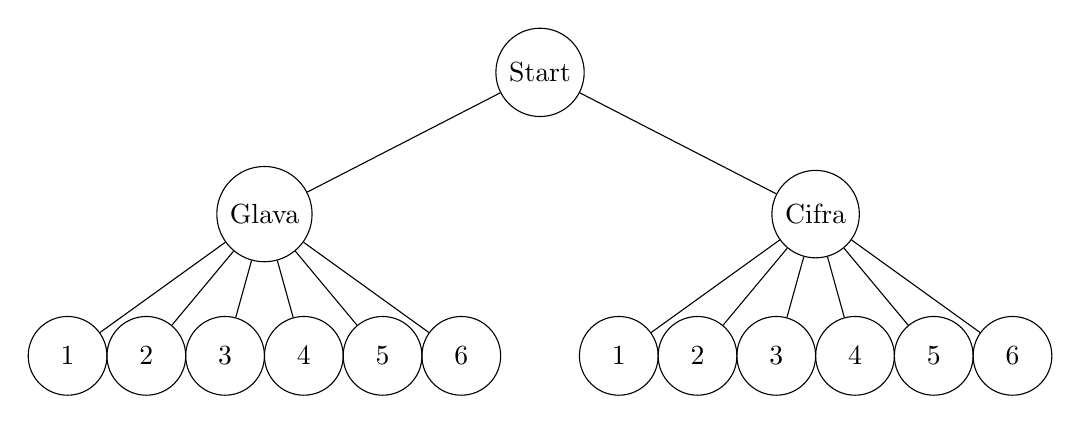
\begin{tikzpicture}[
  level distance=1.8cm,
  level 1/.style={sibling distance=7cm},
  level 2/.style={sibling distance=1cm},
  every node/.style={draw, circle, minimum size=1cm}
]
\node {Start}
  child {node {Glava}
    child {node {1}}
    child {node {2}}
    child {node {3}}
    child {node {4}}
    child {node {5}}
    child {node {6}}}
  child {node {Cifra}
    child {node {1}}
    child {node {2}}
    child {node {3}}
    child {node {4}}
    child {node {5}}
    child {node {6}}};
\end{tikzpicture}
\end{center}

\end{itemize}
}
\end{tabularx}

\razmak{0.5em}


% ******** 95. Permutacije ********
\crta

\naslov{Permutacije}

\begin{tabularx}{\textwidth}{X r}
\vprasanje{Kaj so permutacije brez ponavljanja in koliko jih je?}{2 točki}
\odgovor{
\begin{itemize}
  \item Permutacije brez ponavljanja so razporeditve vseh elementov množice, kjer noben element ni ponovljen.
  \item Če imamo $n$ različnih elementov, je število takšnih permutacij enako $n!$ (``$n$ faktorsko``).
\end{itemize}
}
\end{tabularx}

\begin{tabularx}{\textwidth}{X r}
\vprasanje{Povejte primer permutacije brez ponavljanja.}{1 točka}
\odgovor{
\begin{itemize}
  \item Primer: Permutacije množice $\{1, 2, 3\}$ so npr. $123$, $132$, $213$, $231$, $312$, $321$.
\end{itemize}
}
\end{tabularx}

\begin{tabularx}{\textwidth}{X r}
\vprasanje{Kaj so permutacije s ponavljanjem in koliko jih je?}{2 točki}
\odgovor{
\begin{itemize}
  \item Permutacije s ponavljanjem nastanejo, kadar imamo več enakih elementov.
  \item Če imamo $n$ elementov, med katerimi se $k_1$ elementov ponavlja enako, $k_2$ drugače, ..., potem je število takšnih permutacij:
  \[
    \frac{n!}{k_1! \cdot k_2! \cdot \dots}
  \]
\end{itemize}
}
\end{tabularx}

\begin{tabularx}{\textwidth}{X r}
\vprasanje{Povejte primer permutacije s ponavljanjem.}{1 točka}
\odgovor{
\begin{itemize}
  \item Primer: Permutacije črk v besedi "ANA": $\frac{3!}{2!} = 3$ (ANA, AAN, NAA).
\end{itemize}
}
\end{tabularx}
\razmak{0.5em}


% ******** 96. Variacije ********
\crta

\naslov{Variacije}

\begin{tabularx}{\textwidth}{X r}
\vprasanje{Kaj so variacije brez ponavljanja in koliko jih je?}{2 točki}
\odgovor{
\begin{itemize}
  \item Variacije brez ponavljanja so razporeditve $k$ različnih elementov izmed $n$ različnih elementov, kjer vrstni red šteje in elementi niso ponovljeni.
  \item Število takih variacij je $V(n, k) = \frac{n!}{(n - k)!}$.
\end{itemize}
}
\end{tabularx}

\begin{tabularx}{\textwidth}{X r}
\vprasanje{Povejte primer variacije brez ponavljanja.}{1 točka}
\odgovor{
\begin{itemize}
  \item Primer: Variacije brez ponavljanja dolžine $2$ iz množice $\{A, B, C\}$ so: AB, AC, BA, BC, CA, CB.
\end{itemize}
}
\end{tabularx}

\begin{tabularx}{\textwidth}{X r}
\vprasanje{Kaj so variacije s ponavljanjem in koliko jih je?}{2 točki}
\odgovor{
\begin{itemize}
  \item Variacije s ponavljanjem so razporeditve $k$ elementov izmed $n$ različnih elementov, kjer je vrstni red pomemben, in elementi se ne smejo ponovljati.
  \item Število takih variacij je $V^*(n, k) = n^k$.
\end{itemize}
}
\end{tabularx}

\begin{tabularx}{\textwidth}{X r}
\vprasanje{Povejte primer variacije s ponavljanjem.}{1 točka}
\odgovor{
\begin{itemize}
  \item Primer: Variacije s ponavljanjem dolžine $2$ iz množice $\{A, B\}$ so: AA, AB, BA, BB.
\end{itemize}
}
\end{tabularx}

\razmak{0.5em}


% ******** 97. Kombinacije ********
\crta

\naslov{Kombinacije}

\begin{tabularx}{\textwidth}{X r}
\vprasanje{Kaj je binomski simbol in kako izračunamo njegovo vrednost?}{1 točka}
\odgovor{
\begin{itemize}
  \item Binomski simbol $\binom{n}{k}$ predstavlja število načinov, kako iz množice $n$ različnih elementov izbrati $k$ elementov ne glede na vrstni red.
  \item Izračunamo ga po formuli: $\binom{n}{k} = \frac{n!}{k!(n-k)!}$.
\end{itemize}
}
\end{tabularx}

\begin{tabularx}{\textwidth}{X r}
\vprasanje{Opišite tri lastnosti računanja z binomskimi simboli.}{3 točke}
\odgovor{
\begin{itemize}
  \item $\binom{n}{0} = \binom{n}{n} = 1$ za vsak $n \in \mathbb{N}_0$.
  \item $\binom{n}{k} = \binom{n}{n - k}$ (simetričnost).
  \item $\binom{n-1}{k-1} + \binom{n-1}{k} = \binom{n}{k}$ (Pascalovo pravilo).
\end{itemize}
}
\end{tabularx}

\begin{tabularx}{\textwidth}{X r}
\vprasanje{Kaj so kombinacije brez ponavljanja in koliko jih je?}{1 točka}
\odgovor{
\begin{itemize}
  \item Kombinacije brez ponavljanja so izbire $k$ elementov iz množice $n$ različnih elementov, kjer vrstni red ne igra vloge in elementov ne ponavljamo.
  \item Število takih kombinacij je $\binom{n}{k}$.
\end{itemize}
}
\end{tabularx}

\begin{tabularx}{\textwidth}{X r}
\vprasanje{Povejte primer kombinacije brez ponavljanja.}{1 točka}
\odgovor{
\begin{itemize}
  \item \text{Primer: Iz množice $\{A, B, C\}$ izberemo 2 elementa. Kombinacije so: $\{A, B\}, \{A, C\}, \{B, C\}$.}
\end{itemize}
}
\end{tabularx}

\razmak{0.5em}


% ******** 98. Binomski izrek ********
\crta

\naslov{Binomski izrek}

\begin{tabularx}{\textwidth}{X r}
\vprasanje{Povejte binomski izrek in razčlenite izraz $(a+b)^4$.}{2 točki}
\odgovor{
\begin{itemize}
  \item Binomski izrek: $(a + b)^n = \sum_{k=0}^{n} \binom{n}{k} a^{n-k} b^k$.
  \item Za $n = 4$:
  \[
  (a + b)^4 = \binom{4}{0} a^4 b^0 + \binom{4}{1} a^3 b^1 + \binom{4}{2} a^2 b^2 + \binom{4}{3} a^1 b^3 + \binom{4}{4} a^0 b^4
  \]
  \[
  = a^4 + 4a^3b + 6a^2b^2 + 4ab^3 + b^4
  \]
\end{itemize}
}
\end{tabularx}

\begin{tabularx}{\textwidth}{X r}
\vprasanje{Naj bo $n$ naravno število. Koliko podmnožic ima množica z $n$ elementi?}{1 točka}
\odgovor{
\begin{itemize}
  \item Množica z $n$ elementi ima $2^n$ podmnožic.
\end{itemize}
}
\end{tabularx}

\begin{tabularx}{\textwidth}{X r}
\vprasanje{Opišite povezavo med binomskim izrekom in Pascalovim trikotnikom.}{1 točka}
\odgovor{
\begin{itemize}
  \item Koeficienti v razvoju binomskega izraza $(a + b)^n$ po binomskem izreku so enaki številom v $n$-ti vrstici Pascalovega trikotnika.
\end{itemize}
}
\end{tabularx}

\begin{tabularx}{\textwidth}{X r}
\vprasanje{Opišite dve lastnosti binomskih koeficientov v Pascalovem trikotniku.}{2 točki}
\odgovor{
\begin{itemize}
  \item Vsaka vrstica se začne in konča z $1$.
  \item Vsako notranje število je vsota dveh števil neposredno nad njim: $\binom{n}{k} = \binom{n-1}{k-1} + \binom{n-1}{k}$.
\end{itemize}
}
\end{tabularx}

\razmak{0.5em}


% ******** 99. Verjetnostni račun ********
\crta

\naslov{Verjetnostni račun}

\begin{tabularx}{\textwidth}{X r}
\vprasanje{
Pojasnite osnovne pojme verjetnostnega računa:
\begin{itemize}[leftmargin=*, label={}]
  \item $\rightarrow$ poskus, \hfill (1 točka)
  \item $\rightarrow$ dogodek (slučajni dogodki, nemogoči in gotovi dogodki, elementarni dogodki, sestavljeni dogodki), \hfill \mbox{(2 točki)}
  \item $\rightarrow$ vzorčni prostor. \hfill (1 točka)
  \item Povejte primer poskusa in navedite nekaj dogodkov v tem poskusu. Kateri med njimi so nemogoči, gotovi, elementarni in kateri sestavljeni dogodki? \hfill (2 točki)
\end{itemize}
\vspace{0.5em}
}{6 točk}
\odgovor{
\begin{itemize}
  \item \textbf{Poskus} je dejanje, katerega rezultat je odvisen od naključja in ga opazujemo (npr. met kovanca).
  
  \item \textbf{Dogodek} je rezultat ali množica rezultatov poskusa.
    \begin{itemize}
      \item \textbf{Slučajni dogodek} se lahko zgodi ali pa ne (npr. pade cifra pri metu kovanca).
      \item \textbf{Nemogoči dogodek} se ne more zgoditi (npr. pri metu kovanca pade število 3).
      \item \textbf{Gotovi dogodek} se vedno zgodi (npr. pri metu kovanca pade ali cifra ali grb).
      \item \textbf{Elementarni dogodek} vsebuje natanko en izid (npr. pade cifra).
      \item \textbf{Sestavljeni dogodek} vsebuje več možnih izidov (npr. pri metu kocke pade sodo število).
    \end{itemize}

  \item \textbf{Vzorčni prostor} je množica vseh možnih rezultatov poskusa (npr. pri metu kocke je vzorčni prostor $\Omega = \{1, 2, 3, 4, 5, 6\}$).

  \item \textbf{Primer poskusa:} met standardne igralne kocke.
    \begin{itemize}
      \item \textbf{Elementarni dogodek:} pade število 4.
      \item \textbf{Sestavljeni dogodek:} pade sodo število (2, 4, 6).
      \item \textbf{Nemogoči dogodek:} pade število 7.
      \item \textbf{Gotovi dogodek:} pade število med 1 in 6.
    \end{itemize}
\end{itemize}
}
\end{tabularx}

\razmak{0.5em}


% ******** 100. Verjetnostni račun ********
\crta

\naslov{Verjetnostni račun}

\begin{tabularx}{\textwidth}{X r}
\vprasanje{Definirajte vsoto in produkt dogodkov.}{2 točki}
\odgovor{
\begin{itemize}
  \item \textbf{Vsota dogodkov} $A \cup B$ je dogodek, ki nastopi, če nastopi vsaj eden od dogodkov $A$ ali $B$.
  \item \textbf{Produkt dogodkov} $A \cap B$ je dogodek, ki nastopi, če nastopita oba dogodka hkrati, torej $A$ in $B$.
\end{itemize}
}
\end{tabularx}

\begin{tabularx}{\textwidth}{X r}
\vprasanje{Kdaj sta dva dogodka nezdružljiva in kdaj združljiva? Kako izračunamo verjetnost vsote dveh združljivih dogodkov?}{2 točki}
\odgovor{
\begin{itemize}
  \item \textbf{Nezdružljiva dogodka} sta dogodka, ki ne moreta nastopiti hkrati, torej $A \cap B = \emptyset$.
  \item \textbf{Združljiva dogodka} sta dogodka, ki lahko nastopita hkrati, torej $A \cap B \ne \emptyset$.
  \item \textbf{Verjetnost vsote združljivih dogodkov:}
  \[
  P(A \cup B) = P(A) + P(B) - P(A \cap B)
  \]
\end{itemize}
}
\end{tabularx}

\begin{tabularx}{\textwidth}{X r}
\vprasanje{Kaj je nasprotni dogodek danega dogodka in kako izračunamo njegovo verjetnost?}{1 točka}
\odgovor{
\begin{itemize}
  \item \textbf{Nasprotni dogodek} dogodka $A$ je dogodek $\bar{A}$, ki nastopi, če $A$ ne nastopi.
  \item \textbf{Verjetnost:} $P(\bar{A}) = 1 - P(A)$
\end{itemize}
}
\end{tabularx}

\begin{tabularx}{\textwidth}{X r}
\vprasanje{Povejte primer dveh nezdružljivih dogodkov ter primer dogodka in njemu nasprotnega dogodka.}{1 točka}
\odgovor{
\begin{itemize}
  \item \textbf{Nezdružljiva dogodka:} pri metu kocke dogodka $A$: ``pade 1`` in $B$: ``pade 6`` (ne moreta nastopiti hkrati).
  \item \textbf{Dogodek in nasprotni dogodek:} $A$: ``pade sodo število``, $\bar{A}$: ``pade liho število``.
\end{itemize}
}
\end{tabularx}

\razmak{0.5em}


% ******** 101. Verjetnostni račun ********
\crta

\naslov{Verjetnostni račun}

\begin{tabularx}{\textwidth}{X r}
\vprasanje{Kaj je relativna frekvenca danega dogodka? Definirajte empirično (statistično) verjetnost. Povejte primer.}{2 točki}
\odgovor{
\begin{itemize}
  \item \textbf{Relativna frekvenca} dogodka $A$ je količnik med številom pojavitev dogodka $A$ in številom vseh ponovitev poskusa.
  \[
  f(A) = \frac{n_A}{n}
  \]
  \item \textbf{Empirična verjetnost} dogodka $A$ je približek verjetnosti, dobljen z opazovanjem ali poskusi, in je enaka relativni frekvenci za veliko število ponovitev.
  \item \textbf{Primer:} Če pri 100 metih kovanca pade glava 47-krat, je empirična verjetnost dogodka ``pade glava`` enaka $\frac{47}{100} = 0{,}47$.
\end{itemize}
}
\end{tabularx}

\begin{tabularx}{\textwidth}{X r}
\vprasanje{Povejte klasično (matematično) definioijo verjetnosti. Navedite primer.}{2 točki}
\odgovor{
\begin{itemize}
  \item \textbf{Klasična verjetnost} dogodka $A$ je definirana kot količnik med številom ugodnih izidov za dogodek $A$ in številom vseh enako verjetnih izidov.
  \[
  P(A) = \frac{\text{število ugodnih izidov}}{\text{število vseh možnih izidov}}
  \]
  \item \textbf{Primer:} Pri metu pravilne šeststranske kocke je verjetnost dogodka $A$: ``pade število večje od 4`` enaka:
  \[
  P(A) = \frac{2}{6} = \frac{1}{3}
  \]
\end{itemize}
}
\end{tabularx}

\begin{tabularx}{\textwidth}{X r}
\vprasanje{Povejte dve lastnosti verjetnosti.}{2 točki}
\odgovor{
\begin{itemize}
  \item Verjetnost dogodka $A$ je vedno med 0 in 1: $0 \le P(A) \le 1$.
  \item Verjetnost gotovega dogodka je 1, verjetnost nemogočega dogodka je 0:
  \[
  P(\text{gotovi dogodek}) = 1, \quad P(\text{nemogoči dogodek}) = 0
  \]
\end{itemize}
}
\end{tabularx}

\razmak{0.5em}


% ******** 102. Statistika ********
\crta

\naslov{Statistika}

\begin{tabularx}{\textwidth}{X r}
\vprasanje{
Opišite osnovne statistične pojme:
\begin{itemize}[leftmargin=*, label={}]
  \item $\rightarrow$ populacija in vzorec, \hfill \mbox{(1 točka)}
  \item $\rightarrow$ statistična enota in statistična spremenljivka (znak), \hfill \mbox{(1 točka)}
  \item $\rightarrow$ statistični parameter, \hfill \mbox{(1 točka)}
  \item Na konkretnem primeru statistične raziskave razložite osnovne statistične pojme. \hfill \mbox{(3 točke)}
\end{itemize}
\vspace{0.5em}
}{6 točk}
\odgovor{
\begin{itemize}
  \item \textbf{Populacija} je celota vseh enot, ki jih raziskujemo. \textbf{Vzorček} je podmnožica populacije, ki jo dejansko opazujemo ali merimo.
  \item \textbf{Statistična enota} je posamezni element populacije (npr. oseba, podjetje). \textbf{Statistična spremenljivka (znak)} je lastnost, ki jo pri enotah merimo (npr. višina, starost).
  \item \textbf{Statistični parameter} je številska značilnost populacije (npr. povprečna višina vseh dijakov v državi).
  \item \textbf{Primer:} V raziskavi merimo višino dijakov v Sloveniji.
  \begin{itemize}
    \item Populacija: vsi dijaki v Sloveniji.
    \item Vzorček: 500 dijakov, izbranih iz različnih šol.
    \item Statistična enota: en dijak.
    \item Statistična spremenljivka: višina dijaka.
    \item Statistični parameter: povprečna višina vseh dijakov v Sloveniji.
  \end{itemize}
\end{itemize}
}
\end{tabularx}

\razmak{0.5em}


% ******** 103. Statistika ********
\crta

\naslov{Statistika}

\begin{tabularx}{\textwidth}{X r}
\vprasanje{Definirajte frekvenco in relativno frekvenco dane statistične spremenljivke (znaka).}{2 točki}
\odgovor{
\begin{itemize}
  \item \textbf{Frekvenca} določenega podatka je število pojavitev tega podatka v vzorcu.
  \item \textbf{Relativna frekvenca} je delež pojavitev določenega podatka glede na celotno število podatkov in jo izračunamo kot:
  \[
  \text{relativna frekvenca} = \frac{\text{frekvenca}}{\text{skupno število podatkov}}
  \]
\end{itemize}
}
\end{tabularx}

\begin{tabularx}{\textwidth}{X r}
\vprasanje{Kako izračunamo aritmetično sredino (povprečje) posamičnih podatkov in kako grupiranih podatkov?}{2 točki}
\odgovor{
\begin{itemize}
  \item \textbf{Posamični podatki:}
  \[
  \bar{x} = \frac{x_1 + x_2 + \dots + x_n}{n}
  \]
  kjer je $x_i$ posamezen podatek in $n$ število podatkov.
  \item \textbf{Grupirani podatki:}
  \[
  \bar{x} = \frac{f_1x_1 + f_2x_2 + \dots + f_kx_k}{f_1 + f_2 + \dots + f_k}
  \]
  kjer je $x_i$ središče razreda (sredina intervala), $f_i$ pa frekvenca posameznega razreda.
\end{itemize}
}
\end{tabularx}

\begin{tabularx}{\textwidth}{X r}
\vprasanje{Definirajte modus podatkov. Kako ga določimo?}{2 točki}
\odgovor{
\begin{itemize}
  \item \textbf{Modus} je tisti podatek (ali razred pri grupiranih podatkih), ki se v podatkih pojavi največkrat.
  \item \textbf{Določimo ga} tako, da poiščemo podatek z največjo frekvenco. Če obstaja več takih podatkov, je lahko modus večvreden.
\end{itemize}
}
\end{tabularx}

\razmak{0.5em}


% ******** 104. Statistika ********
\crta

\naslov{Statistika}

\begin{tabularx}{\textwidth}{X r}
\vprasanje{Definirajte mediano podatkov. Kako jo določimo v odvisnosti od števila podatkov?}{2 točki}
\odgovor{
\begin{itemize}
  \item \textbf{Mediana} je srednja vrednost urejenih podatkov.
  \item Če je število podatkov $n$:
  \begin{itemize}
    \item \textbf{liho} ($n$ je liho): mediana je srednji podatek.
    \item \textbf{sodo} ($n$ je sodo): mediana je povprečje dveh srednjih podatkov.
  \end{itemize}
\end{itemize}
}
\end{tabularx}

\begin{tabularx}{\textwidth}{X r}
\vprasanje{Definirajte kvartile. Kaj je medčetrinski razmik?}{2 točki}
\odgovor{
\begin{itemize}
  \item \textbf{Kvartili} razdelijo urejene podatke na štiri enako velike dele:
  \begin{itemize}
    \item $Q_1$ – prvi kvartil: spodnja četrtina (25\%)
    \item $Q_2$ – drugi kvartil: mediana (50\%)
    \item $Q_3$ – tretji kvartil: zgornja četrtina (75\%)
  \end{itemize}
  \item \textbf{Medčetrtinski razmik} je razlika med tretjim in prvim kvartilom:
  \[
  IQR = Q_3 - Q_1
  \]
\end{itemize}
}
\end{tabularx}

\begin{tabularx}{\textwidth}{X r}
\vprasanje{Kako narišemo škatlo z brki? Kolikšen delež podatkov leži med prvim in tretjim kvartilom?}{2 točki}
\odgovor{
\begin{itemize}
  \item \textbf{Škatlo z brki} narišemo tako:
  \begin{itemize}
    \item Na številskem polju označimo $Q_1$, $Q_2$ (mediano) in $Q_3$.
    \item Narišemo škatlo od $Q_1$ do $Q_3$.
    \item V škatli označimo črto za $Q_2$.
    \item Narišemo brke (črte) od škatle do najmanjše in največje vrednosti (brez izstopajočih vrednosti).
  \end{itemize}
  \item \textbf{Delež podatkov} med $Q_1$ in $Q_3$ je približno 50 \%.
\end{itemize}
}
\end{tabularx}

\razmak{0.5em}


% ******** 105. Statistika ********
\crta

\naslov{Statistika}

\begin{tabularx}{\textwidth}{X r}
\vprasanje{Kaj je standardni odklon? Kako ga izračunamo?}{2 točki}
\odgovor{
\begin{itemize}
  \item \textbf{Standardni odklon} meri razpršenost podatkov okoli aritmetične sredine.
  \item Računamo ga kot:
  \[
  s = \sqrt{\frac{1}{n} \sum_{i=1}^{n} (x_i - \bar{x})^2}
  \]
  kjer je $x_i$ posamezni podatek, $\bar{x}$ aritmetična sredina, $n$ število podatkov.
\end{itemize}
}
\end{tabularx}

\begin{tabularx}{\textwidth}{X r}
\vprasanje{Narišite normalno (Gaussovo) krivuljo in na njej označite $\mu$. Kakšen je pomen parametra $\sigma$ ? (Število $\mu$ je srednja vrednost, $\sigma$ pa standardni odklon porazdelitve.)}{2 točki}
\odgovor{
\begin{itemize}
  \item \textbf{$\mu$} je srednja vrednost – krivulja je simetrična glede na $\mu$.
  \item \textbf{$\sigma$} določa razpršenost: večji kot je $\sigma$, širša je krivulja.
  \item Slika: zvonasta krivulja z označeno točko $\mu$ na sredini in točkama $\mu - \sigma$, $\mu + \sigma$ levo in desno.
\end{itemize}
}
\end{tabularx}

\begin{tabularx}{\textwidth}{X r}
\vprasanje{Kolikšen odstotek vrednosti spremenljivke, ki je normalno porazdeljena, leži na intervalu $(\mu-\sigma, \mu+\sigma)$ ?}{1 točka}
\odgovor{
\begin{itemize}
	\item Približno \textbf{68 \%} vseh vrednosti.
\end{itemize}
}
\end{tabularx}

\begin{tabularx}{\textwidth}{X r}
\vprasanje{Kolikšna je ploščina območja med normalno (Gaussovo) krivuljo in abscisno osjo?}{1 točka}
\odgovor{
\begin{itemize}
	\item Ploščina pod celotno krivuljo je \textbf{1} (kar pomeni 100 \% verjetnost).
\end{itemize}
}
\end{tabularx}
\razmak{0.5em}


% Noga...\pagestyle{fancy} pre-uredi dokument...zato je import spodaj
\fancyhf{}                    
\fancyfoot[C]{© Jakob Balkovec}  
\renewcommand{\headrulewidth}{0pt}
\renewcommand{\footrulewidth}{0pt}  
\pagestyle{fancy}

\end{document}